\documentclass{article}

% Packages for code, figures, and automata
\usepackage{listings} % For code listings
\usepackage{graphicx} % For including figures
\usepackage{tikz}     % For drawing automata
\usepackage{multirow}
\usepackage{array}
\usepackage{amssymb} % Pacchetto per simboli matematici
\usepackage{float}
\usepackage{nicematrix}


\usepackage{pgfplots}
\usepackage{amsmath}


%colorize lstlisting with language
\usepackage{xcolor}
\usepackage{titlesec}

%import all important packages 

% Packages for code, figures, and automata
\usepackage{listings} % For code listings
\usepackage{graphicx} % For including figures
\usepackage{tikz}     % For drawing automata
\usepackage{multirow}
\usepackage{array}
\usepackage{amssymb} % Pacchetto per simboli matematici
\usepackage{float}

\usepackage{pgfplots}
\usepackage{amsmath}

%colorize lstlisting with language
\usepackage{xcolor}

\usepackage{titlesec}

%package for theorem
\usepackage{amsthm}
\newtheorem*{theorem}{theorem}

%import all important packages 

% Configurazione degli stili per tutti i linguaggi
\lstset{
    basicstyle=\ttfamily,
    keywordstyle=\color{blue},
    commentstyle=\color{purple},
    stringstyle=\color{red},
    % Altre opzioni
    breaklines=true, showstringspaces=false,
    emph={label},
    emphstyle={\color{custompurple}},
    escapeinside={(*}{*)}
    }

% Stile globale per tutti i linguaggi
\lstdefinestyle{mystyle}{
    backgroundcolor=\color{white},
    commentstyle=\color{purple},
    keywordstyle=\color{blue},
    numberstyle=\tiny\color{gray},
    stringstyle=\color{red},
    basicstyle=\ttfamily\footnotesize,
    breakatwhitespace=false,
    breaklines=true,
    captionpos=b,
    keepspaces=true,
    numbers=left,
    numbersep=5pt,
    showspaces=false,
    showstringspaces=false,
    showtabs=false,
    tabsize=2
}

% Impostazioni per tutti i linguaggi
\lstset{style=mystyle}
% Definizione di simboli per subsection e subsubsection
\newcommand{\subsecsymbol}{\textcolor{custompurple}{\rule[0pt]{10pt}{10pt}\hspace{10pt}}}
\newcommand{\subsubsecsymbol}{\textcolor{custompurple}{\textbf{$\blacklozenge$}\hspace{4pt}}}

\titleformat{\section}[block]
  {\Huge\bfseries}
  {\llap{\textcolor{custompurple}{\rule[-4pt]{10pt}{18pt}\hspace{10pt}}\thesection\hskip 12pt}}
  {0pt}
  {}
% Definizione di uno stile per \subsection
\titleformat{\subsection}[block]
  {\Large\bfseries\color{black}}
  {\llap{\subsecsymbol}\thesubsection\hskip 12pt}
  {0pt}
  {}

% Definizione di uno stile per \subsubsection
\titleformat{\subsubsection}[block]
  {\large\bfseries\color{black}}
  {\llap{\subsubsecsymbol}\thesubsubsection\hskip 12pt}
  {0pt}
  {}


%make link clickable
\usepackage{hyperref}
\usepackage{pgfplots}

%use asmath
\usepackage{amsmath}

\usepackage{fancyhdr}
\pagestyle{fancy}
\fancyhf{}
\fancyhead[R]{\nouppercase{\rightmark}}
\fancyfoot[C]{\thepage}

\usepackage{listings}
\usepackage{tabularx}

%color link orange
\hypersetup{
    colorlinks=true,
    linkcolor=custompurple,
    filecolor=magenta,
    urlcolor=cyan,
}

\definecolor{custompurple}{HTML}{8b3fff}

% Define title and author
\begin{titlepage}
    \title{\color{custompurple}\Huge Deep Learning}
    \author{\textbf{Daniele Avolio}}
\end{titlepage}

\begin{document}

\maketitle
\newpage

\tableofcontents
\newpage
\section{Introduzione}
Info esame: Tecnicamente, per ora rimane un progetto e potrebbe essere di gruppo. Ancora non ci sono informazioni precisissime.






\section{Deep Learning 101}

In questo corso affronteremo diverse tematiche, il che può sembrare assurdo se ci si pensa.

\begin{itemize}
  \item Classificazione (binaria, cioè sì o no)
  \item Multi-class classification (non più binaria)
  \item Regressione (il guessing viene fatto su un valore numerico)
  \item Gestione di immagini e riconoscimento
  \item Serie numeriche (predizioni di mercato e trend)
  \item Classificazione di testi
\end{itemize}

\subsection{Architetture e strumenti nel deep learning}

\begin{itemize}
  \item Autoencoder
    \begin{itemize}
      \item Tutti i possibili tipi
      \item Qui si fa anche \textbf{Clustering} e \textbf{Anomaly detection}
    \end{itemize}
  \item Architetture generative
    \begin{itemize}
      \item Tutti i possibili tipi
    \end{itemize}
  \item XAI: Explainable AI
\end{itemize}

\subsection{Libri utili}
\begin{itemize}
  \item "Deep Learning in Python"
  \item "Tensorflow tutorial"
\end{itemize}

\subsection{Strumenti che useremo}
\begin{itemize}
  \item Tensorflow
    \begin{itemize}
      \item High-level più di altri
    \end{itemize}
  \item Keras
    \begin{itemize}
      \item High-level API basato su Tensorflow
      \item Ci saranno cose che non possiamo fare con Keras perché è troppo ad alto livello
    \end{itemize}
\end{itemize}

\subsection{Schema generale di un problema di deep learning}

Abbiamo delle coppie $(x_0,y_0), (x_1,y_1), (x_2,y_2), \ldots, (x_n, y_n)$ dove $x_i$ è un vettore di features e $y_i$ è un valore numerico (regressione) o una classe (classificazione).

$$y_i = f(x_i)$$

Non conosciamo la funzione $f$, quindi dobbiamo impararla.

$$y = \alpha x + \beta$$

Con una rete neurale puoi approssimare praticamente qualsiasi funzione.

\textit{Una rete neurale permette di collegare un input di dati a una funzione di output.}

Abbiamo diversi tipi di reti neurali a seconda del tipo di problema che vogliamo risolvere. È importante essere in grado di selezionare l'architettura giusta per risolvere il problema.

Definiamo alcuni concetti che useremo:
\begin{itemize}
  \item $N$: rete neurale
  \item $w$: valori dei pesi della rete neurale
  \item $f$: funzione di output della rete neurale
\end{itemize}

$$ f \in N(w)$$

\subsection{Perché si usa il termine "Tensore"?}

Un \textit{tensore} non è altro che una matrice.
\begin{itemize}
  \item 0D tensor: scalar
  \item 1D tensor: vector
  \item 2D tensor: matrix
  \item 3D tensor: tensor
\end{itemize}

\subsection{AI vs DL}

\begin{itemize}
  \item AI: è un ampio insieme di tecniche per risolvere problemi che richiedono "intelligenza".
    \begin{itemize}
      \item Esempio: Stockfish, un programma che gioca a scacchi.
    \end{itemize}
  \item DL: È un sottoinsieme di AI che si concentra sull'\textit{astrazione}.
    \begin{itemize}
      \item L'astrazione consiste nel fornire una funzione che traduce dati di input in dati di output senza conoscere la funzione stessa.
      \item È un approccio induttivo: fornisci un input e ti aspetti un output, senza conoscere la funzione che li collega.
      \item Questo è completamente diverso dall'AI basata sulla logica.
    \end{itemize}
\end{itemize}

\newpage
\section{Introduzione alle Reti Neurali}
\subsection{Il modello di McCulloch-Pitts}
Un modello pensato dai due tizi qui presenti,
\begin{itemize}
    \item Warren McCulloch
    \item Walter Pitts

\end{itemize}

Era formato da:
\begin{itemize}
    \item Un insieme di neuroni
    \item Un insieme di connessioni tra i neuroni
    \item Un insieme di pesi associati alle connessioni
    \item Una funzione di attivazione
    \item Una funzione di output
\end{itemize}

Quindi immaginiamo $x_1, x_2, \dots, x_n$ che vengono dati come input, e quello
che viene fuori è un valore di $y \in \{0,1\}$. Questo è un modello di
classificazione binaria.

In soldoni, in deep learning si usa un vettore di numeri per tirare fuori un
altro vettore di numeri.

Nella maggior parte del tempo, però, non lavoriamo solamente con i dati.
\begin{itemize}
    \item immagini
    \item Testo
    \item Audio
    \item \dots
\end{itemize}
Non ci sono concetti di foto, video, immagini. L'unico concetto che esiste
è quello dei numeri.

\subsection{Modello di Rosenblatt}
Qui il modello è leggermente diverso. Gli elementi in questo modello sono i
seguenti:
\begin{itemize}
    \item Valori di input: $x_i$
    \item Funzione di attivazione: $\phi$
    \item Pesi degli archi: $w_i$
    \item Bias: $b$
\end{itemize}

\begin{equation}
    h(x|w,b) = h(\sum_{i=1}^l w_i\cdot x_i -b) = h(\sum_{i=1}^l w_i\cdot x_i) = \textit{sign}(w^Tx)
\end{equation}

\textbf{Nota:} Quando il \textbf{bias} non viene specificato, allora
si assume che sia 0.

I pesi $w_i$ sono collegati archi che vanno da $x_i$ al prossimo neurone. Sia
il valore di input che il peso sono \textbf{numeri reali}. Non sono lo stesso
valore, hanno solamente il formato di \textit{reale} che è uguale tra loro. Ciò
che viene fatto è solamente la somma della prodotto tra ogni peso $w_i$ e $x_i$
\textbf{meno} il bias.

\textbf{La funzione di attivazione:} Dipende. Ogni funzione che ha \textit{2 stati} va bene per noi. Una funzione di attivazione può essere una qualsiasi che in un
punto ha valore 1 e in un altro ha valore -1.

\subsection{Esempio con 2 neuroni}.

Immaginiamo di avere un piano cartesiano con una retta che interseca in 2
punti.

\begin{equation}
    sign(w_1\cdot x_1 + w_2\cdot x_2)
\end{equation}

Il parametro della funzione non è altro che \textbf{l'equazione di una retta.}

In particolare, se consideriamo la reta che separa gli spazi del piano, vediamo
che la retta è \textbf{capace di separare 2 punti nel piano.}

\textbf{Cosa abbiamo}:
\begin{itemize}
    \item Un neurone
    \item 2 valori in input
    \item 2 pesi
\end{itemize}

Con la funzione di attivazione \textbf{sign} si avrà come output una retta che
separa dei punti.
\begin{tikzpicture}[scale=1.5]
    % Asse x
    \draw[->] (-2,0) -- (2,0) node[right] {$x$};
    % Asse y
    \draw[->] (0,-2) -- (0,2) node[above] {$y$};

    % Punto A
    \coordinate (A) at (-1.5,1);
    \fill[red] (A) circle (2pt) node[above left] {$A$};

    % Punto B
    \coordinate (B) at (1,0.5);
    \fill (B) circle (2pt) node[above right] {$B$};

    % Retta
    \draw[dashed] (-2,-0.25) -- (2,1.75) node[right] {$r$};
\end{tikzpicture}

\textbf{Nota}: Quando è utile avere un valore output che non è una separazione di punti in un piano? Nel caso della \textbf{regressione}.

\textbf{Oltre la funzione sign}:
\begin{itemize}
    \item Funzione di attivazione lineare
    \item Funzione di attivazione sigmoid
    \item Funzione di attivazione Tanh
\end{itemize}

\subsection{Rappresentazione le funzioni logiche}:

\subsubsection{AND}
Immaginiamo di avere:
\begin{itemize}
    \item $x_1,x_2 \in \{0,1\}$
    \item Bias= -30
    \item Funzione di attivazione: Logistica o Sigmoid
\end{itemize}

Come facciamo a rappresentare un AND?

\begin{equation}
    h(x)= g(-30+20x_1 +20x_2)
\end{equation}
\begin{center}
    \begin{tabular}{|c|c|c|}
        \hline
        $x_1$ & $x_2$ & $h(x)$ \\
        \hline
        0     & 0     & 1      \\
        0     & 1     & 0      \\
        1     & 0     & 0      \\
        1     & 1     & 1      \\
        \hline
    \end{tabular}
\end{center}

Lo stesso ragionamento vale per:
\begin{itemize}
    \item OR
    \item NOT
    \item (NOT $x_1$) AND (NOT $x_2$)
\end{itemize}

\subsubsection{Il problema dello XOR}
\begin{quote}
    Il percettrone non può imparare regioni che non sono linearmente separabili.
\end{quote}

\begin{figure}[H]
    \begin{center}
        \begin{tikzpicture}[scale=1.5][h!]
            % Asse x
            \draw[->] (-2,0) -- (2,0) node[right] {$x$};
            % Asse y
            \draw[->] (0,-2) -- (0,2) node[above] {$y$};

            % Punto A
            \coordinate (A) at (0,1);
            \fill[red] (A) circle (2pt) node[above left] {$A$};

            % Punto B
            \coordinate (B) at (0,0);
            \fill (B) circle (2pt) node[above right] {$B$};

            \coordinate (B) at (1,0);
            \fill (B)[red] circle (2pt) node[above right] {$B$};

            \coordinate (B) at (1,1);
            \fill (B) circle (2pt) node[above right] {$B$};
        \end{tikzpicture}
        \caption{XOR non possibile con 1 percettrone}
    \end{center}

\end{figure}

Come vediamo qui non possoamo tracciare una retta per dividere i due punti. In
questo caso ci serve una funzione \textbf{non lineare}.

La soluzione a questo problema è \textbf{aggiungere LAYER} alla rete neurale.
Aggiungere un layer significa aggiungere un neurone successivamente ad un
altro.

Maggiore è il numero di layer, maggiore diventa la potenza espressiva della
rete. Praticamente possiamo catturare qualsiasi cosa aggiungendo layer alla
rete. Questo è \textbf{il vero potere del deep learning}.

\usetikzlibrary{positioning}
\begin{figure}[H]
    \begin{center}

        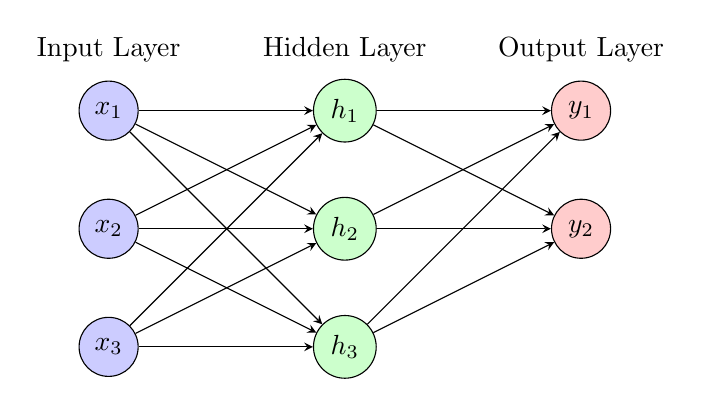
\begin{tikzpicture}[x=1.5cm, y=1.5cm, >=stealth]

            % Input Layer
            \foreach \i in {1,2,3}
            \node[circle, draw, fill=blue!20, minimum size=0.75cm] (I\i) at (0,-\i) {$x_{\i}$};

            % Hidden Layer
            \foreach \i in {1,2,3}
            \node[circle, draw, fill=green!20, minimum size=0.75cm] (H\i) at (2,-\i) {$h_{\i}$};

            % Output Layer
            \foreach \i in {1,2}
            \node[circle, draw, fill=red!20, minimum size=0.75cm] (O\i) at (4,-\i) {$y_{\i}$};

            % Connect Layers
            \foreach \i in {1,2,3}
            \foreach \j in {1,2,3}
            \draw[->] (I\i) -- (H\j);

            \foreach \i in {1,2,3}
            \foreach \j in {1,2}
            \draw[->] (H\i) -- (O\j);

            % Labels
            \node[above=0.5cm] at (I1) {Input Layer};
            \node[above=0.5cm] at (H1) {Hidden Layer};
            \node[above=0.5cm] at (O1) {Output Layer};

        \end{tikzpicture}
    \end{center}
    \caption{Neural Network con 1 hidden layer}
\end{figure}

\subsection{Gli ingredienti di una rete neurale}
\subsubsection{Il grafo g}
Un grafo $g = \{N,E\}$ è un grafo diretto pesato con label.

Ogni nodo $i \in N$ viene chiamato \textbf{neurone} o \textbf{percettrone}. Per
ogni nodo ci sono 2 targhette:
\begin{itemize}
    \item Un valore $a_i$ che viene chiamato \textbf{attivazione}
    \item Una funzione di attivazione $f_i$ che viene applicata all'attivazione, che
          produce un output $z_i$
\end{itemize}

Ogni arco $e = \{j \in N \rightarrow i \in N\} \in E$ associato con un peso
$w_{j,i}$.

Ogni nodo $i$ è anche coinvolto con un arco speciale, con un nodo fantasma, che
viene chiamato \textbf{bias} $b_i$.

\textbf{Nota:} $z_i = f_i(a_i)$. E $a_i = b_i  + \sum_{j:j\rightarrow i \in E} w_{j,i}z_j$

La combinazione dei neuroni connessi costruisce il grafo. I nodi che
condividono gli stessi input sono raggruppati in \textbf{layers}.

\usetikzlibrary{positioning}
\begin{figure}[H]
    \begin{center}

        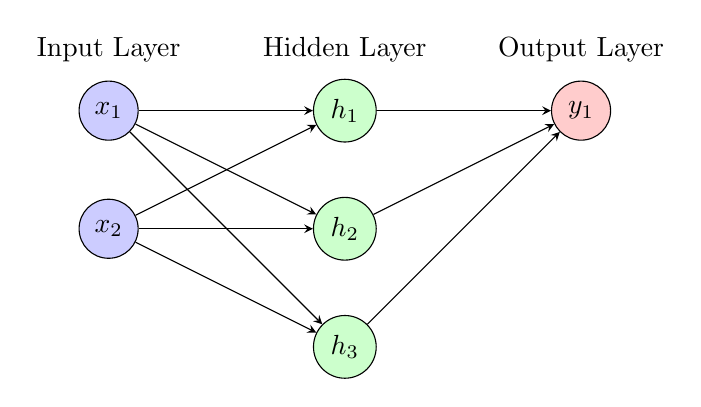
\begin{tikzpicture}[x=1.5cm, y=1.5cm, >=stealth]

            % Input Layer
            \foreach \i in {1,2}
            \node[circle, draw, fill=blue!20, minimum size=0.75cm] (I\i) at (0,-\i) {$x_{\i}$};

            % Hidden Layer
            \foreach \i in {1,2,3}
            \node[circle, draw, fill=green!20, minimum size=0.75cm] (H\i) at (2,-\i) {$h_{\i}$};

            % Output Layer
            \foreach \i in {1}
            \node[circle, draw, fill=red!20, minimum size=0.75cm] (O\i) at (4,-\i) {$y_{\i}$};

            % Connect Layers
            \foreach \i in {1,2}
            \foreach \j in {1,2,3}
            \draw[->] (I\i) -- (H\j);

            \foreach \i in {1,2,3}
            \foreach \j in {1}
            \draw[->] (H\i) -- (O\j);

            % Labels
            \node[above=0.5cm] at (I1) {Input Layer};
            \node[above=0.5cm] at (H1) {Hidden Layer};
            \node[above=0.5cm] at (O1) {Output Layer};

        \end{tikzpicture}
    \end{center}
    \caption{Neural Network con 1 hidden layer}
\end{figure}

Il risultato finale dipende da tutti i parametri del grafo, e anche dal tipo di
funzione di attivazione che viene usata.
\begin{quote}
    Ma come facciamo a scegliere il corretto valore dei parametri del grafo?
\end{quote}

\subsubsection{La funzione di loss}
Il grafo è un operatore algebrico non lineare: $g(\vec{x}|W,B)$. In questo
grafo non sappiamo il valore di \textbf{B e W}. La fase di apprendimenti di una
rete consiste nel trovare il \textbf{migliore} valore per W e per B. Ma cosa
intendiamo con \textbf{migliore?}.

Formalmente, l'unico modo che abbiamo per definire la conezione di migliore, è
quello di \textit{approssimare al meglio la funzione che vogliamo trovare}.

%scrivi un vettore verticale di x_1 a x_m e un vettore verticale di y_1 a y_m%

Consideriamo il valore di una funzione $F$ su $x_i$ e il vero valore di $y_i$.
Noi vogliamo minimizzare la differenza tra $F(x_i)$ e $y_i$.

\begin{equation}
    \min_{W,B}\frac{1}{n} \sum_{i=1}^n loss(\vec{y_i}, g(x_i|W,B))
\end{equation}
con:
\begin{itemize}
    \item $loss(\vec{y_i}, g(x_i|W,B))$ è una funzione che misura la differenza tra $y_i$ e $g(x_i|W,B)$
    \item $n$ è il numero di esempi
    \item $W$ e $B$ sono i parametri del grafo
    \item $g(x_i|W,B)$ è il valore di output del grafo
    \item $\vec{y_i}$ è il valore di output vero
\end{itemize}

La funzione di \textbf{loss} dipende dal tipo di task che dobbiamo svolgere.

\subsubsection{Funzione di loss per Regressione}
\textbf{Mean Absolute Error}:
\begin{equation}
    \frac{1}{n} \sum_{i=1}^n |y_i - g(\vec{x_i}|W,B)|
\end{equation}
\begin{itemize}
    \item Considera tutti gli errori con lo stesso peso
    \item \textbf{Non è differenziabile in 0}
\end{itemize}

\textbf{Mean Squared Error}:
\begin{equation}
    \frac{1}{n} \sum_{i=1}^n (y_i - g(\vec{x_i}|W,B))^2
\end{equation}

\begin{itemize}
    \item Gli errori più grandi hanno un peso maggiore
    \item \textbf{È differenziabile in 0}
    \item \textbf{È più sensibile agli outliers}
\end{itemize}

\textbf{Domanda:} quale si usa tra le due? Dall'approccio greedy, \textbf{usa entrambe}.

\textbf{Esistono anche altre funzioni:}
\begin{itemize}
    \item Smooth Absolute Error
    \item Huber Loss
\end{itemize}

\subsubsection{Funzione di loss per classificazione}

\textbf{Binary Cross Entropy [BCE]}
Viene usata se $y_i \in \{0,1\}, g(\vec{x}|W,B) \in [0,1]$.
\begin{equation}
    BCE = -\frac{1}{n} \sum_{i=1}^n y_i \log(g(\vec{x_i}|W,B)) - (1-y_i)\log(1-g(\vec{x_i}|W,B))
\end{equation}

\textbf{Categorical Cross Entropy [CCE]}
Da scrivere.

\subsection{L'ottimizzatore o}
Come risolviamo il problema di:
\begin{equation}
    \min_{W,B} \frac{1}{n} \sum_{i=1}^n loss(\vec{y_i}, g(\vec{x_i}|W,B))
\end{equation}

Il problema lo risolviamo calcolando il \textbf{gradiante} della funzione loss,
lo poniamo uugale a 0 e controlliamo se siamo in un punto di \textbf{massimo,
    minimo o punto di sella}.

\begin{tikzpicture}
    \begin{axis}[
            xlabel=$x$,
            ylabel=$f(x)$,
            domain=-2:2,
            samples=200,
            axis lines=middle,
            width=10cm,
            height=6cm,
            xmin=-2,
            xmax=2,
            ymin=-4,
            ymax=5,
            xtick={-1, 0, 1},
            xticklabels={$-1$, $0$, $1$},
            ytick={1, 3},
            yticklabels={$f_{\text{min}}$, $f_{\text{max}}$},
        ]

        \addplot[blue,thick,domain=-1.5:1.5] {x^4 - 2*x^3 - 2*x^2 + 3*x + 1};
    \end{axis}
\end{tikzpicture}

Abbiamo bisogno di un metodo iterativo per trovare una soluzione. Ci vuole
un'\textbf{euristica}. Tipicamente, siamo soddisfatti di un \textbf{minimo
    locale}, e si utilizza, appunto, il \textbf{metodo di discesa del gradiente}.

\subsubsection{Il metodo di discesa del gradiente}
Sia $F(\vec{x})$ una funzione differenziabile.
\begin{itemize}
    \item $F(\vec{x})$ decresce più veloce nella direzione del gradiente negativo
    \item $F(\vec{x})$ cresce più veloce nella direzione opposta al gradiente
\end{itemize}

\begin{equation}
    a^{new} = a^{old} - \eta \cdot \nabla F(a^{old})
\end{equation}

Il parametro $\eta$ viene chiamato \textbf{learning rate} e determina il
comportamento del'ottimizzazione.
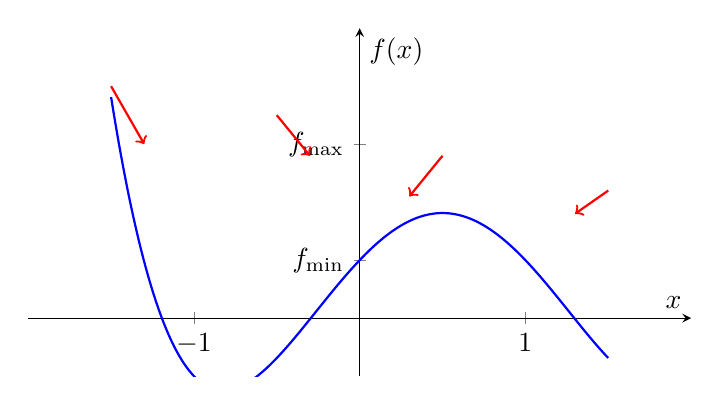
\begin{tikzpicture}
    \begin{axis}[
            xlabel=$x$,
            ylabel=$f(x)$,
            domain=-2:2,
            samples=200,
            axis lines=middle,
            width=10cm,
            height=6cm,
            xmin=-2,
            xmax=2,
            ymin=-1,
            ymax=5,
            xtick={-1, 0, 1},
            xticklabels={$-1$, $0$, $1$},
            ytick={1, 3},
            yticklabels={$f_{\text{min}}$, $f_{\text{max}}$},
        ]

        \addplot[blue,thick,domain=-1.5:1.5] {x^4 - 2*x^3 - 2*x^2 + 3*x + 1};

        % Frecce verso il minimo
        \draw[->, red, thick] (axis cs:-1.5,4) -- (axis cs:-1.3,3);
        \draw[->, red, thick] (axis cs:-0.5,3.5) -- (axis cs:-0.3,2.8);
        \draw[->, red, thick] (axis cs:0.5,2.8) -- (axis cs:0.3,2.1);
        \draw[->, red, thick] (axis cs:1.5,2.2) -- (axis cs:1.3,1.8);

    \end{axis}
\end{tikzpicture}

\textbf{Ci sono ancora problemi:} Questo metodo non è esente da problemi, quindi abbiamo:
\begin{itemize}
    \item Dipendentemente dal punto di inizio, abbiamo un risultato diverso. Dobbiamo
          capire che, giustamente, se ci accontentiamo di un minimo locale, non avremo
          quasi mai lo stesso minimo per ogni allenamento della rete.
\end{itemize}

Diciamo che in generale, gli steps per allenare una rete sono:
\lstset{mathescape}
\begin{lstlisting}
    for each topology T in $C_t$
        for each $\eta$ in $C_\eta$
            for each initialization I in $C_I$
                Applica la discesa del gradiente
\end{lstlisting}

\subsubsection{Il metodo di discesa del gradiente stocastico}
La differenza del metodo di discesa del gradiente stocastico è che, invece di
calcolare il gradiente su tutti i dati, si calcola il gradiente su un
sottoinsieme di dati.

Ciò che viene fatto, per ogni step, invece di prendere la derivata di ogni loss
function e poi fare i calcoli, prendo \textbf{un sample del mio dataset},
tipicamente chiamato \textbf{batch}. Ogni volta che calcolo la discesa del
gradiente, calcolo la derivata \textbf{NON PER TUTTO IL DATASET}, ma solamente
del \textbf{batch}. Questo OVVIAMENTE non mi assicura che ottimizzare ogni
batch mi ottimizza anche l'intero dataset, ma non c'è modo di lavorare
sull'intero dasaset, poiché questo è troppo grande e richiede troppo tempo.

Nonostante tutto, utilizzando questa tecnica \textbf{si ottengono risultati
    comunque accettabili}.

Il \textit{workflow} allora cambia in: \lstset{mathescape}
\begin{lstlisting}
    for each topology T in $C_t$
        for each $\eta$ in $C_\eta$
          for each initialization I in $C_I$
           for each batch size $b \in C_b$
             Applica la discesa del gradiente stocastica
\end{lstlisting}

\subsubsection{Linee guida sul learning rate}

\textbf{Epoca}: Un'epoca è un passaggio dell'approssimazione della funzione

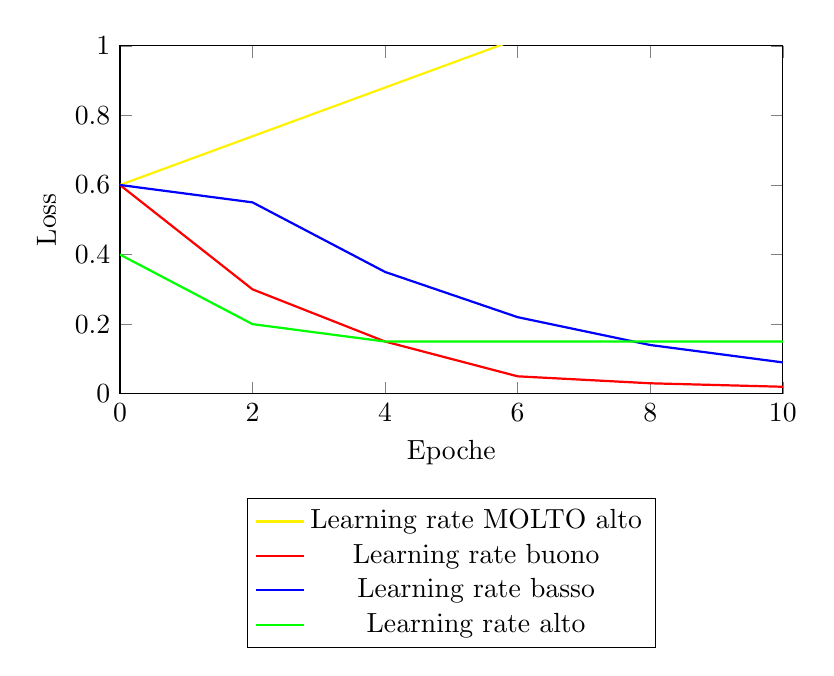
\begin{tikzpicture}
    \begin{axis}[
            xlabel=Epoche,
            ylabel=Loss,
            width=10cm,
            height=6cm,
            xmin=0,
            xmax=10,
            ymin=0,
            ymax=1,
            xtick={0, 2, 4, 6, 8, 10},
            ytick={0, 0.2, 0.4, 0.6, 0.8, 1},
            legend style={at={(0.5,-0.3)},anchor=north},
            legend entries={Learning rate MOLTO alto, Learning rate buono, Learning rate basso, Learning rate alto},
        ]

        \addplot[thick, yellow] coordinates {(0, 0.6) (10, 1.3)};
        \addplot[thick, red] coordinates {(0, 0.6) (2, 0.3) (4, 0.15) (6, 0.05) (8, 0.03) (10, 0.02)};
        \addplot[thick, blue] coordinates {(0, 0.6) (2, 0.55) (4, 0.35) (6, 0.22) (8, 0.14) (10, 0.09)};
        \addplot[thick, green] coordinates {(0, 0.4) (2, 0.2) (4, 0.15) (6, 0.15) (8, 0.15) (10, 0.15)};

    \end{axis}
\end{tikzpicture}

\textbf{Nota:} Il learning rate è un parametro che va \textbf{tunato}.
\begin{itemize}
    \item Se il learning rate è troppo alto, non si riesce a convergere poiché si
          salta il minimo
    \item Se il learning rate è troppo basso, si rischia di non convergere mai
\end{itemize}

Il nostro obiettivo è quello di avere un learning rate che sia \textbf{giusto} e che permetta di avere un andamento della funzione di loss come quello in rosso, cioé avere una buona
diminuizione della loss andando avanti con le epoche. Sempre decrescente e con la distanza minore dall'asse delle x.

\textbf{Domanda:} Vogliamo sempre la loss uguale a 0? \textbf{No.}
Perché? Perché a differenza che in statistica dove vogliamo avere un errore il minimo.
In deep learning non è così. Se la loss è 0, allora vuol dire che la rete ha
imparato a memoria i dati, e non è quello che vogliamo. Vogliamo che la rete
sia capace di generalizzare.

In particolare, noi \textbf{vogliamo fare predizioni}, sopratutto su \textbf{istanze ancora non viste.} Se avessimo una loss uguale a 0, probabilmente non 
saremmo in grado di avere delle predizioni decenti, poiché la rete non è in grado di generalizzare.
Avendo la loss non a 0 rendiamo la rete capace di poter introdurre istanze ancora non viste in futuro.

Quindi, per statistica \textbf{loss = 0 : nice}, per \textbf{deep learning: insomma}.


\begin{tikzpicture}
    \begin{axis}[
        xlabel=$x$,
        ylabel=$y$,
        width=12cm, % Larghezza maggiore
        height=6cm,
        xmin=0,
        xmax=10,
        ymin=0,
        ymax=1,
        xtick={0, 2, 4, 6, 8, 10},
        ytick={0, 0.2, 0.4, 0.6, 0.8, 1},
    ]
    
    \addplot[thick, blue, smooth] coordinates {(0, 1) (2, 0.5) (4, 0.3) (8, 0)};
    \end{axis}
    \end{tikzpicture}
\newpage
\section{Classificazione Binaria}
\textbf{Descrizione di cosa andremo a fare:} utilizziamo il dataset IMDb Dataset.
Questo dataset è un Database compilato dagli utenti del sito. Le caratteristiche, in particolare, sono:
\begin{itemize}
    \item 50.000 recensioni
    \item circa 50\% positive e 50\% negative
    \item \textit{25.000} sono usate per il \textbf{training} e \textit{25.000} sono usate per il \textbf{testing}. Anche queste sono il 50\% positive e 50\% negative.
\end{itemize}

La task che faremo su questo dataset prende il nome di \textbf{sentimental
    analysis}, ovvero analisi del sentimento.

\textbf{Assunzione:} Ciò che stiamo facendo ha senso solamente se assumiamo \textit{che nel futuro avremo punti con una distribuzione abbastanza simile a quelli utilizzati per il training}.

La partizione di \textbf{test} è una partizione che non viene utilizzata per la
fase di training, ma viene utilizzata successivamente per controllare se il
modello si sta comportando bene nella predizione dei valori. Ci sono delle
misure che hanno range $[0,1]$ che ci permettono di capire quanto il modello si
sta comportando bene.

\textbf{Nota:} il \textit{test set} non viene fornito quando si lavora nel deep learning, altrimenti verrebbe usato per ottimizzare direttamente il modello. \textbf{Non si conosce inizialmente.}

% BEGIN: xz8c6549bwf9
\begin{figure}[H]
    \centering
    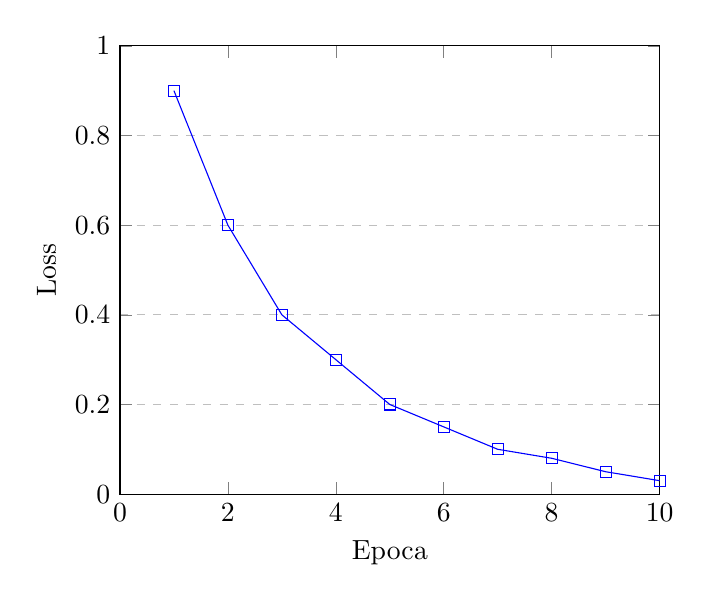
\begin{tikzpicture}
        \begin{axis}[
                xlabel={Epoca},
                ylabel={Loss},
                xmin=0, xmax=10,
                ymin=0, ymax=1,
                xtick={0,2,4,6,8,10},
                ytick={0,0.2,0.4,0.6,0.8,1},
                legend pos=north east,
                ymajorgrids=true,
                grid style=dashed,
            ]
            \addplot[
                color=blue,
                mark=square,
            ]
            coordinates {
                    (1,0.9)(2,0.6)(3,0.4)(4,0.3)(5,0.2)(6,0.15)(7,0.1)(8,0.08)(9,0.05)(10,0.03)
                };
        \end{axis}
    \end{tikzpicture}
    \caption{Grafico di una curva di loss che diminuisce all'aumentare delle epoche.}
    \label{fig:loss_curve}
\end{figure}
% END: xz8c6549bwf9

\subsection{Caricamento e gestione del Dataset}

\begin{lstlisting}[language=Python, caption=Caricamento del dataset IMDb Dataset.]
from keras.datasets import imdb
(train_data, train_labels), (test_data, test_labels) = imdb.load_data(num_words=10000)
\end{lstlisting}

\begin{itemize}
    \item training\_data: sono gli input del training
    \item training\_labels: sono gli output del training
    \item test\_data: sono gli input del test
    \item test\_labels: sono gli output del test
\end{itemize}

% BEGIN: 7z5t8f6d4xw3
\begin{figure}[H]
    \centering
    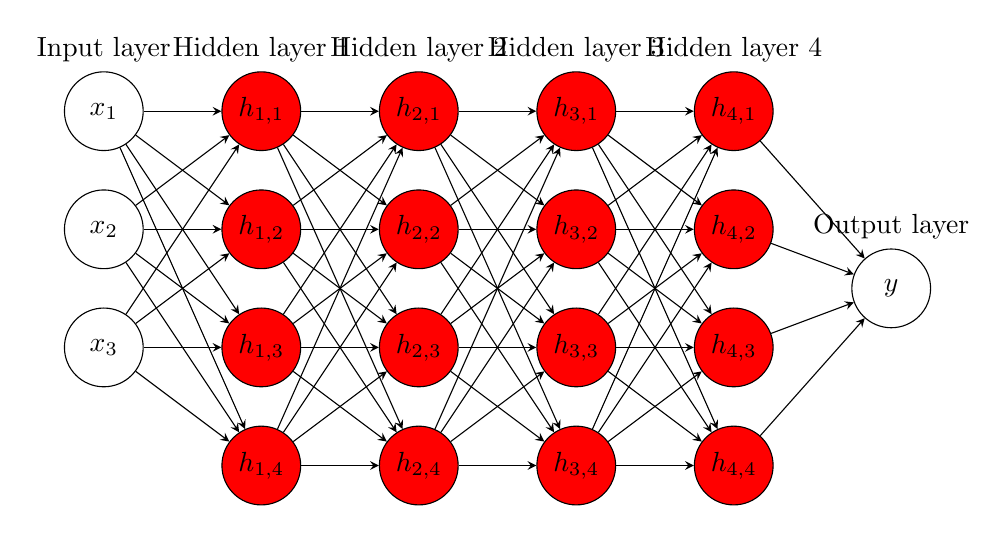
\begin{tikzpicture}[x=1cm, y=1.5cm, >=stealth]
        % Input layer nodes
        \foreach \i in {1,...,3}
        \node[circle, draw=black, fill=white, inner sep=0pt, minimum size=10mm] (I-\i) at (0,-\i) {$x_\i$};

        % Hidden layer nodes
        \foreach \i in {1,...,4}
        \node[circle, draw=black, fill=red, inner sep=0pt, minimum size=10mm] (H1-\i) at (2,-\i) {$h_{1,\i}$};
        \foreach \i in {1,...,4}
        \node[circle, draw=black, fill=red, inner sep=0pt, minimum size=10mm] (H2-\i) at (4,-\i) {$h_{2,\i}$};
        \foreach \i in {1,...,4}
        \node[circle, draw=black, fill=red, inner sep=0pt, minimum size=10mm] (H3-\i) at (6,-\i) {$h_{3,\i}$};
        \foreach \i in {1,...,4}
        \node[circle, draw=black, fill=red, inner sep=0pt, minimum size=10mm] (H4-\i) at (8,-\i) {$h_{4,\i}$};

        % Output layer nodes
        \node[circle, draw=black, fill=white, inner sep=0pt, minimum size=10mm] (O) at (10,-2.5) {$y$};

        % Connections
        \foreach \source in {1,...,3}
        \foreach \dest in {1,...,4}
        \draw[->] (I-\source) -- (H1-\dest);
        \foreach \source in {1,...,4}
        \foreach \dest in {1,...,4}
        \draw[->] (H1-\source) -- (H2-\dest);
        \foreach \source in {1,...,4}
        \foreach \dest in {1,...,4}
        \draw[->] (H2-\source) -- (H3-\dest);
        \foreach \source in {1,...,4}
        \foreach \dest in {1,...,4}
        \draw[->] (H3-\source) -- (H4-\dest);
        \foreach \source in {1,...,4}
        \draw[->] (H4-\source) -- (O);

        % Labels
        \node[above] at (I-1.north) {Input layer};
        \node[above] at (H1-1.north) {Hidden layer 1};
        \node[above] at (H2-1.north) {Hidden layer 2};
        \node[above] at (H3-1.north) {Hidden layer 3};
        \node[above] at (H4-1.north) {Hidden layer 4};
        \node[above] at (O.north) {Output layer};
    \end{tikzpicture}
    \caption{Neural network with 3 input nodes, 4 hidden layers with 3 nodes each, and 1 output layer with 1 node.}
    \label{fig:neural_network}
\end{figure}

Quali sono i primi problemi che vanno gestiti in questo caso? Abbiamo il
problema che i \textbf{dati sono parole e non numeri}. Quindi dobbiamo
trasformare le parole in numeri.

Ogni parola viene \textbf{trasformato} in un numero. Ci troviamo però con delle
recensioni che sono delle \textbf{sequenze di parole}, e quindi abbiamo delle
\textbf{sequenze di numeri}. La soluzione è quelal di usare un \textbf{set di
    parole codificate.} Mi spiego:

Immaginiamo di avere 10.000 parole encodate. Salvo queste 10.000 parole in un
array e associo ad ogni parola un indice di questo array.

\begin{figure}[H]
    \begin{center}
        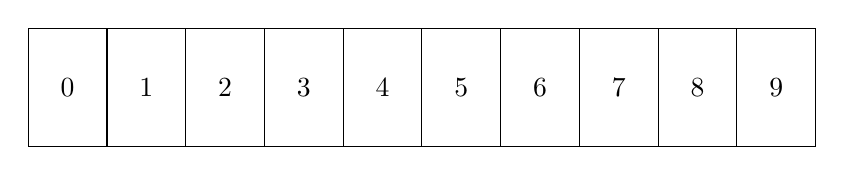
\begin{tikzpicture}[x=1cm, y=1.5cm, >=stealth]
            \draw (0,0) rectangle (10,1);
            \draw (0,0) rectangle (1,1);
            \draw (1,0) rectangle (2,1);
            \draw (2,0) rectangle (3,1);
            \draw (3,0) rectangle (4,1);
            \draw (4,0) rectangle (5,1);
            \draw (5,0) rectangle (6,1);
            \draw (6,0) rectangle (7,1);
            \draw (7,0) rectangle (8,1);
            \draw (8,0) rectangle (9,1);
            \draw (9,0) rectangle (10,1);
            \node at (0.5,0.5) {0};
            \node at (1.5,0.5) {1};
            \node at (2.5,0.5) {2};
            \node at (3.5,0.5) {3};
            \node at (4.5,0.5) {4};
            \node at (5.5,0.5) {5};
            \node at (6.5,0.5) {6};
            \node at (7.5,0.5) {7};
            \node at (8.5,0.5) {8};
            \node at (9.5,0.5) {9};
        \end{tikzpicture}

    \end{center}
\end{figure}

Ora, cosa manca? \textbf{Manca l'ordine}. L'unica cosa che abbiamo è quindi una
indicizzazione delle parole, ma non abbiamo alcuna informazione dell'ordine.
\textbf{Manca anche totalmente la semantica}.

La struttura dell'input è quindi un \textbf{livello con 10.000 nodi di input.s}

\textbf{Input}
\begin{lstlisting}[language=Python]
import numpy as np
def vectorize_sequences(sequences, dimension=10000):
# Create an all-zero matrix of shape (len(sequences), dimension)
results = np.zeros((len(sequences), dimension))
for i, sequence in enumerate(sequences):
    results[i, sequence] = 1. # set specific indices of results[i] to 1s
return results
# Our vectorized training data
x_train = vectorize_sequences(train_data)
# Our vectorized test data
x_test = vectorize_sequences(test_data)

\end{lstlisting}

\textbf{Output}
\begin{lstlisting}[language=Python]
# Our vectorized labels
y_train = np.asarray(train_labels).astype('float32')
y_test = np.asarray(test_labels).astype('float32')

\end{lstlisting}

\subsection{Definizione della Rete Neurale}
\textbf{Codice iniziale della definizione della Rete}

\begin{lstlisting}[language=Python]
    from keras import models
from keras import layers
model = models.Sequential()
model.add(layers.Dense(16, activation='relu', input_shape=(10000,)))
model.add(layers.Dense(16, activation='relu'))
model.add(layers.Dense(1, activation='sigmoid'))
model.compile(optimizer='rmsprop', 
            loss='binary_crossentropy',
             metrics=['accuracy'])
\end{lstlisting}

Il \textbf{modello sequenziale} è quello migliore da dove iniziare. Cosa
significa però modello sequenziale? Il modello sequenziale ha il concetto di
\textbf{layer}. Ha la funzione \textbf{add} che aggiunge un layer sopra gli
altri layer che sono già esistenti.

\textbf{Primo Layer:}

\textit{layers.Dense}: un layer denso significa che ogni nodo di quel layer è collegato con ogni nodo del layer precedente. \textbf{16} è il numero di neuroni che si vogliono attivare in quel layer.
input\_shape è la dimensione dell'input. \textbf{10000} è la dimensione dell'input. Notare che si ha una \textbf{virgola} nell'input dopo il 10.000 e indica che \textit{che stiamo aspettando una sequenza di vettori, ognuno di dimensione 10.000}
Cioè, praticamente stiamo dicendo \textbf{10.000} sono le parole per ogni recensione, e con la virgola stiamo dicendo che \textbf{non sappiamo quante recensioni abbiamo}.E' comodo quando non abbiamo un numero
fisso di example del dataset da processare.

\textbf{Quante connessioni ci sono?} \[16 \cdot 10000 + 16 = 160016\] dove sono 16 i bias.

\textbf{Cosa significa relu?} ReLu è la funzione di attivazione.

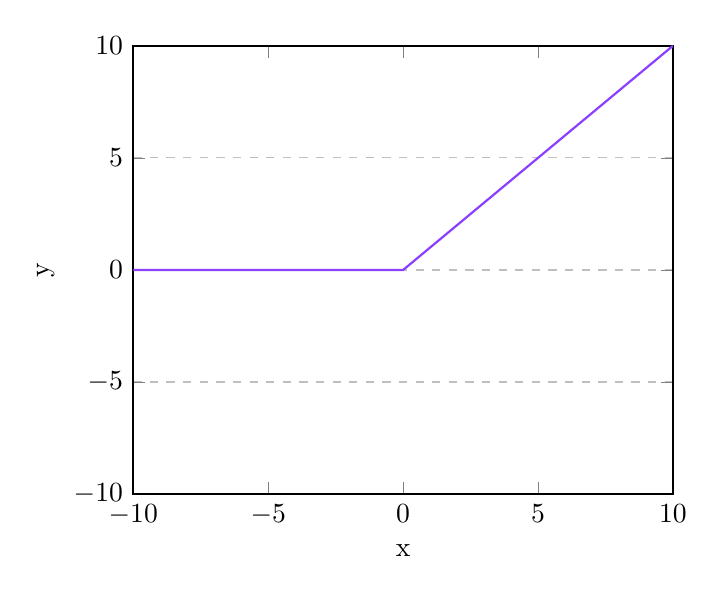
\begin{tikzpicture}
    \begin{axis}[
            xlabel={x},
            ylabel={y},
            xmin=-10, xmax=10,
            ymin=-10, ymax=10,
            xtick={-10,-5,0,5,10},
            ytick={-10,-5,0,5,10},
            legend pos=north east,
            ymajorgrids=true,
            grid style=dashed,
            thick
        ]
        \addplot[
            color=custompurple,
            thick
        ]
        coordinates {
                (-10,0)(-9,0)(-8,0)(-7,0)(-6,0)(-5,0)(-4,0)(-3,0)(-2,0)(-1,0)(0,0)(1,1)(2,2)(3,3)(4,4)(5,5)(6,6)(7,7)(8,8)(9,9)(10,10)
            };
    \end{axis}
\end{tikzpicture}

E' una funzione di attivazione artificiale che fino a 0 è 0, e poi cresce
linearmente. E' una funzione che si usa molto in deep learning.

\textbf{Secondo layer}:

Nel secondo layer abbiamo altri \textbf{16} nodi connessi con i precedenti 16
nodi. In tutto abbiamo \[16 \cdot 16 + 16 = 272\] connessioni, con 16 che sono i bias.

\textbf{Layer di output}:

In questo layer abbiamo un unico nodo connesso con i 16 nodi precedenti. In
tutto abbiamo \[16 \cdot 1 + 1 = 17\] connessioni, con 1 che è il bias. La funzione di attivazioe è la
\textbf{sigmoid}, che è una funzione che ha range $[0,1]$ che indica la
probabilità che il dato appartenga alla classe 1.

Diciamo che è stato osservato che la \textit{sigmoid è meglio nell'output}.
Perché? Eh funziona cosi a quanto pare lol.

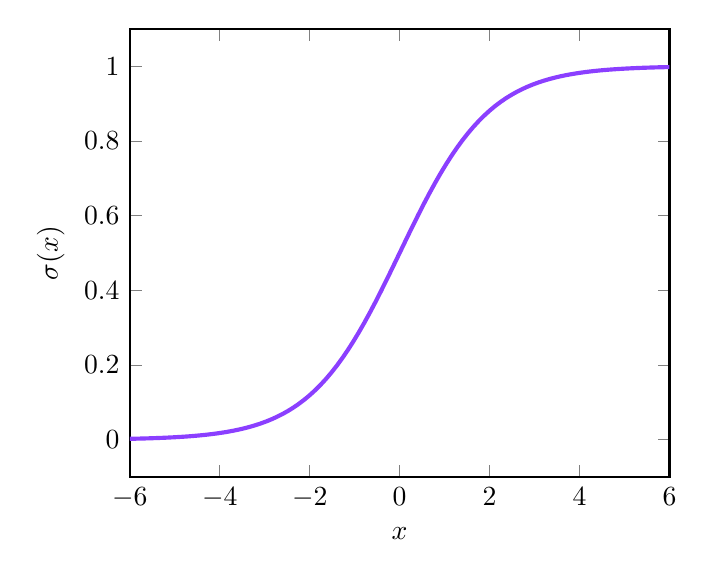
\begin{tikzpicture}
    \begin{axis}[
            xlabel=$x$,
            ylabel=$\sigma(x)$,
            xmin=-6, xmax=6,
            ymin=-0.1, ymax=1.1,
            samples=100,
            thick,
            every axis plot/.append style={line width=1.5pt}
        ]
        \addplot[custompurple,domain=-6:6] {1/(1+exp(-x))};
    \end{axis}
\end{tikzpicture}

\textbf{Compilazione del modello}

In questa sezione si definisce il \textbf{loss} e l'\textbf{optimizer}.

L'ottimizzatore sarebbe, praticamente, la \textit{discesa del gradiente}. Ci
sono vari ottimizzatori ed è molto buono per te stesso provare gli
ottimizzatori e vedere quale funziona meglio per il tuo problema. Letteralmente
il deep learning :) Per quanto riguarda la loss abbiamo visto nella scorsa
sezione le funzioni di loss che conosciamo.

La \textbf{metrica} è quella che viene usata per valutare effettivamente il
modello. In questo caso si usa l'\textbf{accuracy} che praticamente è la
percentuale di classificazioni corrette.

\subsection{Plotting del modello}

E' un plotting molto base e non molto fancy, ma fa il suo lavoro diciamo
\begin{lstlisting}[language=Python]
from keras.utils import plot_model
plot_model(model, show_shapes=True, show_layer_names=True)
    
\end{lstlisting}

\begin{figure}[H]
    \centering
    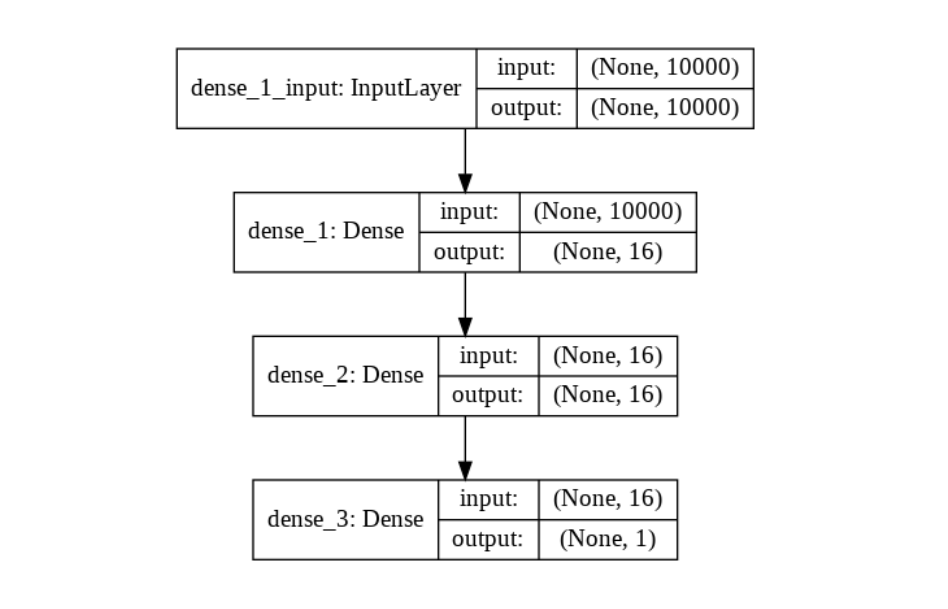
\includegraphics[width=0.8\linewidth]{images/plot res.png}
    \caption{Plotting del modello.}
    \label{fig:plot_model}
\end{figure}

\subsection{Training del modello e valutazione}

Entra in gioco il concetto di \textbf{validation set}.

\subsubsection{Validation Set}
Quando ho un modello, come faccio a sapere se la rete che sto allenando si sta
allenando in modo corretto? Tutto questo sapendo che \textbf{non abbiamo
    accesso al test set}. Pensiamo al \textbf{training set} e pensiamo ad un altro
\textbf{split} interno al training set:
\begin{itemize}
    \item Training set parziale
    \item Validation set
\end{itemize}

Quindi se avessimo 50.000 di grandezza del dataset:
\begin{itemize}
    \item 25.000 test set
    \item 25.training set
          \begin{itemize}
              \item 10.000 validation set
              \item 15.000 training set parziale
          \end{itemize}
\end{itemize}

\begin{lstlisting}
x_val = x_train[:10000]
partial_x_train = x_train[10000:]
y_val = y_train[:10000]
partial_y_train = y_train[10000:]

\end{lstlisting}

Praticamente è come se usassimo il validation come se fosse un test set. Quindi
andremo a plottare 2 curve:
\begin{itemize}
    \item La loss sulle epoche
    \item L'accuracy sulle epoche
\end{itemize}

\textbf{La loss} ci da un'idea di quanto il modello si sta allenando bene. Se ci sono problemi, la figura è strana e non segue un andamento corretto, si modifica.
Ma la cosa importante è la \textbf{validation accuracy}, che DEVE essere crescere in modo monotono e deve avvicinarsi a 1 il più possibile.

%grafico loss
\begin{figure}[H]
    \centering
    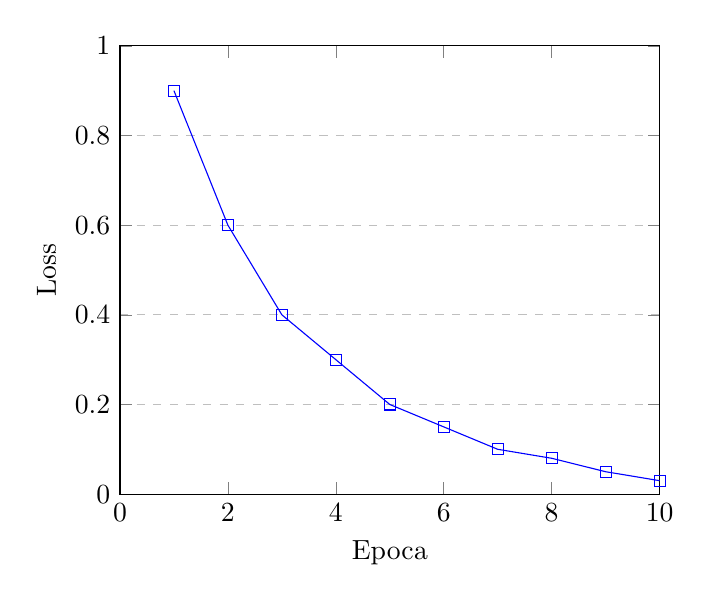
\begin{tikzpicture}
        \begin{axis}[
                xlabel={Epoca},
                ylabel={Loss},
                xmin=0, xmax=10,
                ymin=0, ymax=1,
                xtick={0,2,4,6,8,10},
                ytick={0,0.2,0.4,0.6,0.8,1},
                legend pos=north east,
                ymajorgrids=true,
                grid style=dashed,
            ]
            \addplot[
                color=blue,
                mark=square,
            ]
            coordinates {
                    (1,0.9)(2,0.6)(3,0.4)(4,0.3)(5,0.2)(6,0.15)(7,0.1)(8,0.08)(9,0.05)(10,0.03)
                };
        \end{axis}
    \end{tikzpicture}
    \caption{Grafico di una curva di loss che diminuisce all'aumentare delle epoche.}
    \label{fig:loss_curve}
\end{figure}

%grafico accuracy
\begin{figure}[H]
    \centering
    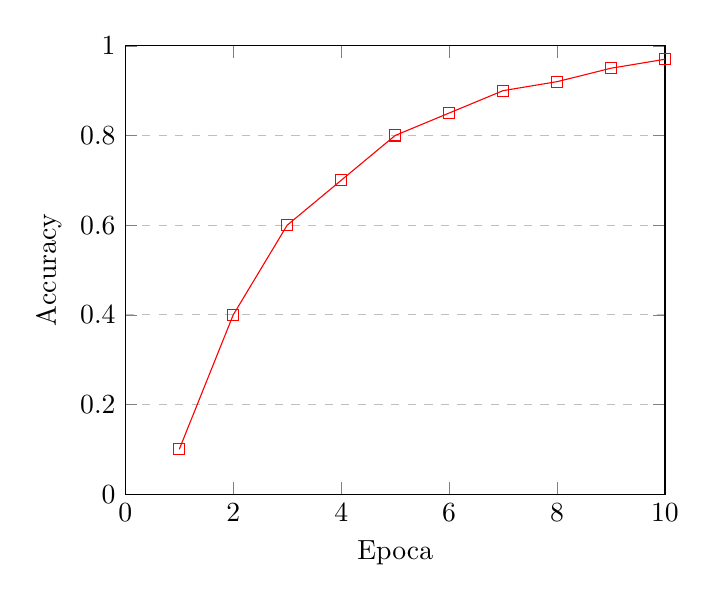
\begin{tikzpicture}
        \begin{axis}[
                xlabel={Epoca},
                ylabel={Accuracy},
                xmin=0, xmax=10,
                ymin=0, ymax=1,
                xtick={0,2,4,6,8,10},
                ytick={0,0.2,0.4,0.6,0.8,1},
                legend pos=north east,
                ymajorgrids=true,
                grid style=dashed,
            ]
            \addplot[
                color=red,
                mark=square,
            ]
            coordinates {
                    (1,0.1)(2,0.4)(3,0.6)(4,0.7)(5,0.8)(6,0.85)(7,0.9)(8,0.92)(9,0.95)(10,0.97)
                };
        \end{axis}
    \end{tikzpicture}
    \caption{Grafico di una curva di accuracy che aumenta all'aumentare delle epoche.}
    \label{fig:accuracy_curve}
\end{figure}

Ma anche se avessimo queste curve inìcon questa conformazione, \textbf{ancora
    non ci dice niente}. Il validation è in un senso insensato per l'output. Ciò
che importerà sarà il \textbf{test set} che non è stato usato per il training.

\textbf{Training code}

\begin{lstlisting}[language=Python]
history = model.fit(partial_x_train,
            partial_y_train,
            epochs=20,
            batch_size=512,
            validation_data=(x_val, y_val))
\end{lstlisting}

\textbf{Plotting delle curve}

Notare che questo è un plotting molto base e non molto fancy, e in futuro
utilizzeremo \textbf{Tensorboard} che aggiornerà in tempo reale i grafici

\begin{lstlisting}[language=Python]
import matplotlib.pyplot as plt
loss = history.history['loss']
val_loss = history.history['val_loss']
epochs = range(1, len(loss) + 1)
# "bo" is for "blue dot"
plt.plot(epochs, loss, 'bo', label='Training loss')
# b is for "solid blue line"
plt.plot(epochs, val_loss, 'b', label='Validation loss')
plt.title('Training and validation loss')
plt.xlabel('Epochs')
plt.ylabel('Loss')
plt.legend()
plt.show()
\end{lstlisting}

Notare che \textit{history} è un dizionario e si può accedere come indicato a
riga \textit{1 e 2} come accedere a loss e val\_loss.
\begin{figure}[H]
    \centering
    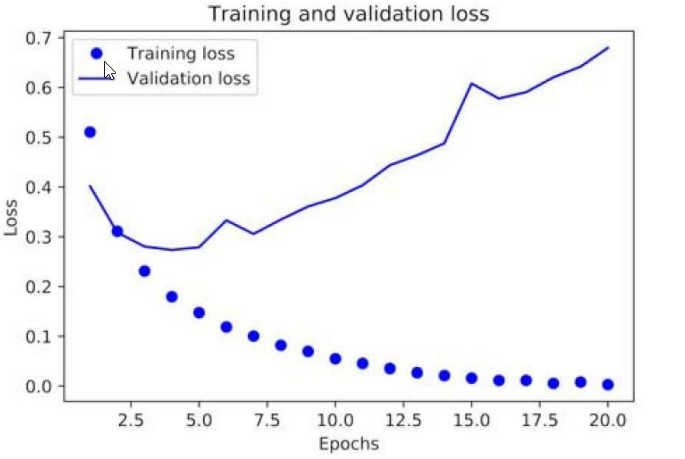
\includegraphics[width=0.8\linewidth]{images/wrong network.png}
    \caption{Rete sbagliata}
    \label{fig:loss}
\end{figure}

Un grafico del genere ci mostra una rete che \textbf{funziona male}!.

\begin{lstlisting}[language=Python]
plt.clf() # clear figure
acc = history_dict['binary_accuracy']
val_acc = history_dict['val_binary_accuracy']
plt.plot(epochs, acc, 'bo', label='Training acc')
plt.plot(epochs, val_acc, 'b', label='Validation acc')
plt.title('Training and validation accuracy')
plt.xlabel('Epochs')
plt.ylabel('Accuracy')
plt.legend()
plt.show()

\end{lstlisting}

\begin{figure}[H]
    \centering
    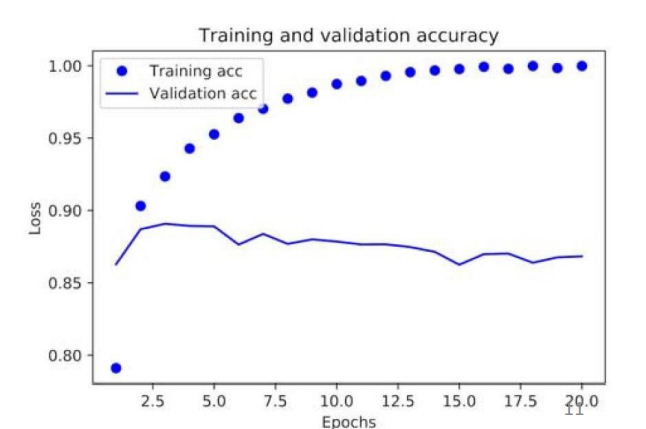
\includegraphics[width=0.8\linewidth]{images/overfitting.png}
    \caption{Overfitting}
    \label{fig:overfitting}
\end{figure}

In questo caso la rete ha un problema di \textbf{overfitting!}.

\subsection{Prediction}
\begin{lstlisting}
model.predict(x_test)
\end{lstlisting}
\[array([[ 0.91966152], [ 0.86563045], [ 0.99936908], ..., [ 0.45731062], [
                    0.0038014 ], [ 0.79525089]], dtype=float32\]

\subsection{Come risolvere problemi di accuracy bassa?}
Se quando andiamo a fare la validazione della nostra rete, come sappiamo come
modificare qualcosa per rendere la rete migliore? Ci sono alcuni approcci per
farlo:
\begin{itemize}
    \item Cambiare la topologia
    \item Diminuire le epoche
    \item Cambiare il numero di nodi per qualche layer
    \item FORSE cambiare anche il learning rate
\end{itemize}

Si noti che facendo questo vanno interpretati i grafici per capire come sta
andando la rete. Quando cominciamo a vedere che la \textbf{validation accuracy}
\textbf{NON STA SOLAMENTE CRESCENDO} ma ci sono dei punti in cui diminuisce,
siamo sicuri che \textbf{c'è qualche problema di mezzo.} Bisogna capire anche
su cosa lavorare. Se cambiando i dati spesso la \textbf{validation accuracy}
mostra problemi, allora bisogna lavorare per quello e cercare di trovare un
modo per fare in modo che il problema non si presenti.

\textbf{RECAPPONE}: Se notiamo che nella LOSS ci sono problemi, possiamo tunare il \textbf{learning rate} e altri
parametri per cercare di risolvere questi problemi. Ma la cosa più importante è \textbf{la metrica}. Se notiamo che
la \textbf{metrica non rispecchia un andamento di effettivo apprendimento}, capiamo che la rete non si sta comportando nel modo corretto
e non sta funzionando.

\subsection{Early Stopping}

E' un metodo che consiste nel vedere quando \textbf{la loss} comincia ad avere
dei comportamenti sospetti. Quando si \textbf{ferma} la rete in un dato
momento, si impedisce alla rete di \textbf{overfittare} nella maggior parte dei
casi.

\section{Classificazione Multiclasse}

Questa sezione sarà molto corta, poiché praticamente è la stessa cosa della
classificazione binaria, ma il layer finale della rete non sarà composto da un
solo nodo, ma da \textbf{un numero di nodi pari al numero di classi da
    classificare}.

\subsection{Descrizione del dataset - Reuters}

Il dataset che verrà utilizzato è il \textbf{Reuters Dataset}, che è un dataset
di \textbf{news} che sono state classificate in \textbf{46 categorie}. Ogni
categoria ha almeno 10 esempi nel training set.

\textbf{Preprocessing dell'input}

\begin{lstlisting}[language=Python]
import numpy as np
def vectorize_sequences(sequences, dimension=10000):
    results = np.zeros((len(sequences), dimension))
    for i, sequence in enumerate(sequences):
        results[i, sequence] = 1.
    return results
# Our vectorized training data
x_train = vectorize_sequences(train_data)
# Our vectorized test data
x_test = vectorize_sequences(test_data)
\end{lstlisting}

\subsubsection{Come processiamo l'output?}

Nel deep learning, \textbf{gli output categorici} non vengono mai mappati ad
una scala numerica. Si utilizza una tecnica che si chiama \textbf{one hot
    encoding}.

\textbf{One Hot Encoding}:

Consiste nel creare tante variabili numeriche quanti sono i valori della
variabile categorica, e per quel dato example viene assegnato
\begin{itemize}
    \item 1: se il valore della variabile categorica è quello
    \item 0: se il valore della variabile categorica non è quello, quindi in tutti gli altri casi
\end{itemize}

Da notare che il one hot encoding viene fatto sia per le labels di output, ma
non è sbagliato farlo anche per gli attributi in alcuni casi.

\begin{lstlisting}[language=Python]
def to_one_hot(labels, dimension=46):
    results = np.zeros((len(labels), dimension))
    for i, label in enumerate(labels):
        results[i, label] = 1.
    return results
# Our vectorized training labels
one_hot_train_labels = to_one_hot(train_labels)
# Our vectorized test labels
one_hot_test_labels = to_one_hot(test_labels)

#OPPURE ALLO STESSO MODO

from keras.utils.np_utils import to_categorical

one_hot_train_labels = to_categorical(train_labels)
one_hot_test_labels = to_categorical(test_labels)
\end{lstlisting}

\textbf{Nota}: nel one hot encoding DOBBIAMO AVERE 1 SOLO VALORE per il dato example, e tutti gli altri non devono essere attivi.
La domanda è, quindi, \textbf{quale activation function usiamo?}

\textit{Immaginiamo questa situazione}: Abbiamo $y_1, y_2, y_3$ che sono i valori di output. Vogliamo solamente uno dei tre.
Se normalizzassimo i dati in questo modo:
\begin{itemize}
    \item $p_1 = \frac{y_1}{y_1+y_2+y_3}$
    \item $p_2 = \frac{y_2}{y_1+y_2+y_3}$
    \item $p_3 = \frac{y_3}{y_1+y_2+y_3}$
\end{itemize}

E se sommiamo $p_1+p_2+p_3$ otteniamo 1. Quindi, in questo caso, possiamo usare
la \textbf{softmax} come activation function.

\subsubsection{Softmax activation function}

Se prendiamo un vettore $\vec{y} = (y_1, y_2, y_3)$, la softmax è definita
come:

\begin{equation}
    S(y_i) = \frac{e^{y_i}}{\sum_{j=1}^{3} e^{y_j}}
\end{equation}

In output abbiamo: $\vec{p} = (p_1, p_2, p_3)$, dove $p_i$ è la probabilità che
il dato example appartenga alla classe $i$.

Nota: quando dividiamo qualcosa, abbiamo \textbf{sempre} un problema riguardo
la stabilità numerica. La divisione è molto critica, poiché \textbf{potrebbe
    essere vicina a 0}. Sappiamo che se usiamo $e^y_1 + e^y_2 + e^y_3$
difficilmente si avvicina a 0.

\begin{lstlisting}[language=Python]
    from keras import models
    from keras import layers
    model = models.Sequential()
    model.add(layers.Dense(64, activation='relu', input_shape=(10000,)))
    model.add(layers.Dense(64, activation='relu'))
    model.add(layers.Dense(46, activation='softmax'))
    model.compile(optimizer='rmsprop',
                loss='categorical_crossentropy',
                metrics=['accuracy'])
\end{lstlisting}

\textbf{Nota:} Dobbiamo avere un numero di nodi di output quanto il numero di classi,
ma \textbf{altra cosa}, il numero di nodi interni deve essere sicuramente
maggiore di 46, altrimenti ci sarebbe una perdita di informazioni.

\textbf{Nota 2:} La funzione di attivazione dell'ultimo layer è una \textbf{softmax}.

\textbf{Validation set e Training set}
\begin{lstlisting}[language=Python]
   
x_val = x_train[:1000]
partial_x_train = x_train[1000:]
y_val = one_hot_train_labels[:1000]
partial_y_train = one_hot_train_labels[1000:]
history = model.fit(partial_x_train,
                partial_y_train,
                epochs=20,
                batch_size=512,
                validation_data=(x_val, y_val))
\end{lstlisting}

\textbf{Loss}

\begin{lstlisting}[language=Python]
import matplotlib.pyplot as plt
loss = history.history['loss']
val_loss = history.history['val_loss']
epochs = range(1, len(loss) + 1)
plt.plot(epochs, loss, 'bo', label='Training loss')
plt.plot(epochs, val_loss, 'b', label='Validation loss')
plt.title('Training and validation loss')
plt.xlabel('Epochs')
plt.ylabel('Loss')
plt.legend()
plt.show()
\end{lstlisting}

\textbf{Accuracy}

\begin{lstlisting}[language=Python]
plt.clf() # clear figure
acc = history.history['acc']
val_acc = history.history['val_acc']
plt.plot(epochs, acc, 'bo', label='Training acc')
plt.plot(epochs, val_acc, 'b', label='Validation acc')
plt.title('Training and validation accuracy')
plt.xlabel('Epochs')
plt.ylabel('Acc')
plt.legend()
plt.show()

\end{lstlisting}

\textbf{Nota:} L'accuracy è importante dipendentemente dall'utilizzo che bisogna farne.
Ad esempio, \textit{in ambito medico} vogliamo \textbf{minimizzare i falsi negativi}. Questo implica
che la misura che usiamo dipende dall'applicazione che se ne fa.
\newpage
\section{Giochi Competitivi o Non Cooperativi}

I giochi competitivi o non cooperativi sono i più studiati. Si assume che un
numero di agenti agisca strategicamente e sia interessato solo al proprio
guadagno, senza collaborare. Cosa succede quando ogni agente ha un obiettivo e
alcuni interessi, e forse alcuni di essi sono in contrasto?

Abbiamo un insieme di agenti che chiamiamo $N$ (per esempio $N =
    \{1,2,\ldots\}$). Ognuno di essi ha alcune azioni possibili tra cui scegliere,
quindi abbiamo un insieme di azioni $A_i$ che è un sottoinsieme di tutte le
possibili azioni $A_i \subset A$ (per esempio $A_i = \{p, q, \ldots\}$). Quando
scegliamo un'azione, otteniamo un valore per questa azione, e c'è un premio
associato che è un numero reale. Questo premio dipende non solo dalle nostre
azioni ma anche dalle azioni degli altri giocatori, quindi il valore dipende da
noi e dagli altri agenti.

Ciascun agente è associato a un'utilità $u_i$ che dipende da tutte le
strategie:
\[u_i : A_1 \times A_2 \times A_3 \times \ldots \times A_n \to \mathbb{R}\]

Il nostro obiettivo è massimizzare la nostra utilità, ma non possiamo
ottimizzare completamente poiché non possiamo controllare le variabili degli
altri giocatori. Dobbiamo anche considerare cosa giocheranno gli altri
giocatori.

Consideriamo un gioco con due giocatori, Bob e John. Le azioni disponibili sono
$\{HOME, OUT\}$. Cosa succede quando eseguono queste azioni? Di solito,
mettiamo l'utilità di entrambi gli agenti in una matrice:

\[
    \begin{array}{ccc}
                    & \text{HOME} & \text{OUT} \\
        \text{HOME} & (1, 2)      & (1, 0)     \\
        \text{OUT}  & (2, 0)      & (-1, 3)    \\
    \end{array}
\]

In questo esempio, i numeri rappresentano le preferenze mappate su numeri
reali.

Cosa significa questo? Sono una mappatura delle preferenze in numeri reali.
Quale sarebbe l'esito? Di solito non è facile capire cosa accadrà.

\[
    \begin{array}{ccc}
                    & \text{HOME} & \text{OUT} \\
        \text{HOME} & (2, 2)      & (1, 1)     \\
        \text{OUT}  & (1, 0)      & (0, 0)     \\
    \end{array}
\]

In questo esempio, l'equilibrio di Nash è \{HOME, HOME\}, poiché questo esito è
fortemente preferito tra gli scenari. Ma cosa succede in questo caso?

\[
    \begin{array}{ccc}
                    & \text{HOME} & \text{OUT} \\
        \text{HOME} & (2, 2)      & (1, 3)     \\
        \text{OUT}  & (1, 0)      & (0, 0)     \\
    \end{array}
\]

(1,3) è un equilibrio di Nash. (2,0) è un equilibrio di Nash.

\subsection{Equilibrio di Nash in Giochi Puri}

Una strategia $s_i$ per un agente è un'azione, in cui scegliamo una delle
azioni disponibili. Un profilo di strategia congiunta o $\sigma$ è una
strategia per ciascun agente del gioco. $\sigma$ è un equilibrio di Nash se,
per ciascun agente possibile, l'utilità dell'agente ($u(\sigma)$) ottenuta per
una particolare strategia che decide di giocare dovrebbe essere almeno uguale o
maggiore dell'utilità che potrebbe ottenere se gli altri giocassero la stessa
strategia, ma lui prova una nuova strategia. In altre parole, giocando una
strategia diversa mentre gli altri mantengono le stesse strategie, dovrebbe
ottenere lo stesso valore o un valore maggiore. $\sigma = (\sigma_i$ che è
$s_i$, $\sigma_{-i}$ è la strategia degli altri).

Questo tipo di equilibrio e impostazione è chiamato "puro". Un esempio può
aiutare a capire il concetto:

\[
    \begin{array}{ccc}
                    & \text{HOME} & \text{OUT} \\
        \text{HOME} & (1, 2)      & (1, 0)     \\
        \text{OUT}  & (2, 0)      & (-1, 3)    \\
    \end{array}
\]

In questo caso, non esiste un equilibrio di Nash, nessuno è davvero felice, e
c'è una situazione ciclica. Quando ci concentriamo sull'equilibrio di Nash,
possiamo avere uno, più di uno o nessuno.

Per calcolare un equilibrio di Nash, è necessario iterare tra le strategie
degli agenti e tra le strategie di ciascun agente. Il limite è dominato dalla
dimensione del prodotto cartesiano: $|A_1 \times A_2 \ldots \times A_n| \times
    |N| \times \max|A_i| \geq 2^n$. Ciò rende difficile rappresentare matrici
quando il numero di agenti è grande, poiché la dimensione della
rappresentazione è esponenziale rispetto al numero di agenti.

\subsection{Equilibrio di Nash in Giochi Grafici}

Ma cosa succede con l'equilibrio di Nash in giochi non puri? Supponiamo di
avere un grande gioco di popolazione, interagirai davvero con tutti i
partecipanti al gioco? Invece, interagirai con i tuoi vicini (amici e nemici),
quindi creerai un grafo con nodi che corrispondono esattamente agli agenti.
L'utilità dipende dalle tue azioni e dalle azioni dei tuoi vicini. Questo è
noto come "giochi grafici". I tuoi vicini sono un sottoinsieme di $N$ e sono i
nodi adiacenti. La funzione di utilità è $u_i : A_i \times \prod_{j \in
        \text{neigh}_i} A_j \to \mathbb{R}$. Se hai al massimo $k$ agenti intorno a te,
allora sappiamo che la dimensione (la matrice, l'utilità) è di circa $O(2^k)$,
ma poiché $k$ è limitato, questa rappresentazione è ragionevole.

Tuttavia, è importante notare che anche se non sei direttamente connesso, gli
altri influenzano comunque i tuoi vicini, quindi alla fine è necessario
considerare tutti i giochi e tutti gli agenti.

\subsection{Complessità Computazionale}

Consideriamo il problema: esiste un equilibrio di Nash in un gioco grafico
(IMPOSTAZIONE PURA)? Siamo in NP? - Dobbiamo indovinare un profilo di
strategia, il che richiede tempo polinomiale, quindi la dimensione di $\sigma$
è polinomiale rispetto alle dimensioni dei giochi. - Verifica se il profilo di
strategia è un equilibrio di Nash: dobbiamo iterare su tutti gli agenti
possibili e su tutte le possibili azioni $|N| \times |A_i|$, il che è anch'esso
polinomiale.

Quindi sappiamo che questo problema è in NP. Ma è anche NP-hard?

Supponiamo di avere due agenti e tre azioni:

\[
    \begin{array}{cccc}
          & R     & G     & B     \\
        R & (0,0) & (1,1) & (1,1) \\
        G & (1,1) & (0,0) & (1,1) \\
        B & (1,1) & (1,1) & (0,0) \\
    \end{array}
\]

\subsection{Esempio di Equilibrio di Nash}

In questo esempio, cerchiamo di capire come ottenere un equilibrio di Nash in
un gioco usando un esempio di colorazione di grafo. Supponiamo che vogliamo che
due agenti, a e b, siano felici solo se scelgono colori diversi. Abbiamo tre
colori: Rosso (R), Verde (G) e Blu (B).

\[
    \begin{array}{cccccccc}
          &   &       & a     &       &            &       & \\
          &   & R     &       & G     &            & B     & \\
        a & R & (0,0) & (1,1) & (1,1) & (1/2, 1/2)           \\
          & G & (1,1) & (0,0) & (1,1)                        \\
          & B & (1,1) & (1,1) & (0,0)                        \\
          & U &       &       &       &            & (2,2)   \\
          &   & R     &       & G     &            & B     & \\
          &   &       & b     &       &            &       & \\
    \end{array}
\]

In questo modo, possiamo sempre far sì che gli agenti siano felici quando
scelgono colori diversi. Supponiamo che il grafo sia 3-colorabile, il che
significa che è possibile colorare i nodi in modo che nessun nodo adiacente
abbia lo stesso colore. In questo caso, esiste un equilibrio di Nash.

Supponiamo ora che il grafo non sia 3-colorabile, il che significa che ci
saranno sempre due nodi che sceglieranno lo stesso colore, ma per uno di loro
non sarà conveniente cambiarlo. Questo "ingranaggio" potrebbe non funzionare,
ma potrebbe sempre esistere un equilibrio di Nash.

Inoltre, aggiungiamo un'ulteriore variabile, $U$, che rappresenta la situazione
in cui non è possibile ottenere un colore diverso e quindi giochiamo $U$. In
questa situazione, se un vicino sta giocando $U$, vogliamo anche noi giocare
$U$. Ma in questo modo potremmo finire in un equilibrio di Nash in cui tutti
giocano $U$, il che non vogliamo. Per affrontare questa situazione, aggiungiamo
    un giocatore fittizio, detto anche "dummy player", che non è felice a giocare
$U$, ma si preoccupa solo se qualcun altro sta giocando $U$. Abbiamo quindi due
    giocatori, $\alpha$ e $\beta$, che giocheranno come segue:

\[
    \begin{array}{ccc}
               & \alpha & \beta  \\
        \alpha & (1,-1) & (-1,1) \\
        \beta  & (-1,1) & (1,-1) \\
    \end{array}
\]
In questo modo, otteniamo un'utilità che non scatena una situazione di
soddisfacibilità. Pertanto, assumendo che il grafo non sia 3-colorabile,
potrebbe non esistere un equilibrio di Nash.

\newpage
\section{Metodi di decomposizione strutturale e Isole di tracciability per problemi NP-Hard}

Stiamo partendo da questo grafico per quanto riguarda il \textbf{Kakutani's
    fixed point theorem}:

\begin{figure}[H]
    \centering
    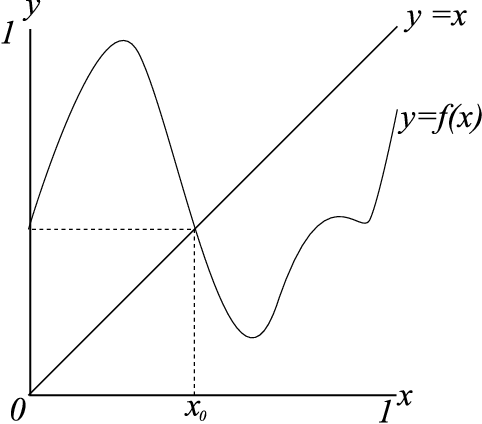
\includegraphics[width=0.7\linewidth]{chapters/images/13-Figure1.1-1.png}
    \caption{}
    \label{fig:1}
\end{figure}

dove sull'asse delle $x$ abbiamo la \textbf{probabilità di fare un'azione}, e
sull'asse delle $y$ la nuova probabilità di eseguire quell'azione.

\[
    x \rightarrow y
\]

ma x e y sono la stessa cosa. E' una funzione che va in se stessa.

Il momento in cui si interseca la bisezione del quadrante, sei sicuro che
\textbf{quel punto esiste} e che quel punto è un \textbf{equilibrio di Nash}.

Non ho la minima idea di cosa stia succedendo qui, ma vediamo cosa ha da dire
chat.

\textit{Risposta di Copilot Chat:}

Nella teoria dei giochi, il teorema del punto fisso di Kakutani è usato per
dimostrare l'esistenza dell'equilibrio di Nash. Un equilibrio di Nash è una
situazione in cui nessun giocatore può migliorare il proprio risultato
cambiando unilateralmente la propria strategia, dato che le strategie degli
altri giocatori rimangono invariate.

La connessione tra il teorema del punto fisso di Kakutani e l'equilibrio di
Nash è la seguente: si può pensare a ogni strategia come a un punto in uno
spazio, e a ogni risposta ottimale a una strategia come a un altro punto in
quello spazio. L'equilibrio di Nash corrisponde a un punto fisso in questo
spazio: un punto che è mappato su se stesso dalla funzione che assegna a ogni
strategia la sua risposta ottimale.

In altre parole, l'equilibrio di Nash è una situazione in cui la "migliore
risposta" di ogni giocatore alla strategia degli altri è semplicemente la
strategia che sta già giocando. Questo è esattamente il tipo di situazione che
il teorema del punto fisso di Kakutani è progettato per gestire, quindi può
essere usato per dimostrare che un tale equilibrio deve esistere.

Nei giochi \textbf{puri}, \textit{trovare} un equilibro di nash è
\textbf{NP-Complete}. E nel caso dei giochi \textbf{misti}, in quale
complessità siamo?

Nei giochi misti sappiamo subito che la risposta è \textbf{si!}, ma dalla
\textit{proof} si vede che non è facile trovare il valore di $f$. In
letteratura, si è visto che in questi casi si può ottenere un equilibro di nash
con valore \textit{irrazionale}, come $\frac{1}{\sqrt{2}}$.

\begin{equation}
    \begin{aligned}
        a_i , b_i, c_i                                     \\
        \text{utility} = f(\sum a_i \times b_i \times c_i) \\
        \text{Si può ottenere } \sqrt{3}
    \end{aligned}
\end{equation}

E alla lavagna ha scritto, rispettivamente come per i giochi puri
\textbf{np-complete}, per i giochi misti ha scritto \textbf{computazione}.

\subsection{PPAD} ( Polynomial Parity Argument on Directed Graphs )

C'è un grafo particolare per questa complessita, che è il seguente:

%6 nodi, 4 hanno un ciclo, il terzo va ad un altro nodo, questo altro nodo va in un altro e uno va fuori, l'altro nodo va al 4o

A quanto pare navigare questo grafo era importante e rappresentava qualcosa, ma
purtroppo non ho capito perché è letteralmente andato come un razzo e non c'è
assolutamenteniente su internet di quello che diceva Greco.

\subsection{Tree Decomposition}

Partiamo a parlare di complessità esponenziale. L'esempio principale è quello
del \textbf{domino}. Il domino è un gioco che si gioca con delle tessere, che
hanno due numeri da 0 a 6, e si devono mettere in fila in modo che i numeri
combacino. Il gioco è finito quando non si possono più mettere tessere in fila.

In generale, dato un insieme di tessere, siamo in grado di mettere in uno
spazio limitato? Si, è NP-Hard: si guessa e si controlla. Ma se vogliamo fare
la stessa cosa per uno spazio senza limiti, come facciamo? Il problema è
esponenziale.

\begin{esempio}(3 colorabilità)
\end{esempio}

\begin{itemize}
    \item Input: Un grafo $G$
    \item Domanda: Il grafo $G$ è 3-colorabile?
\end{itemize}

%disegna un grafo 3 colorabile
\begin{figure}[H]
    \begin{center}
        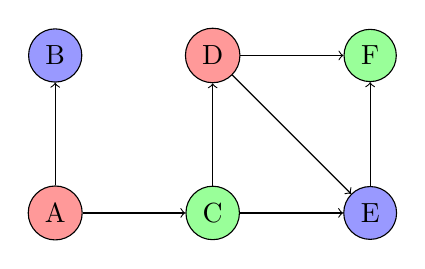
\begin{tikzpicture}
            \node[shape=circle,draw=black,fill=red!40] (A) at (0,0) {A};
            \node[shape=circle,draw=black,fill=blue!40] (B) at (0,2) {B};
            \node[shape=circle,draw=black,fill=green!40] (C) at (2,0) {C};
            \node[shape=circle,draw=black,fill=red!40] (D) at (2,2) {D};
            \node[shape=circle,draw=black,fill=blue!40] (E) at (4,0) {E};
            \node[shape=circle,draw=black,fill=green!40] (F) at (4,2) {F};
            \path [->] (A) edge node[left] {} (B);
            \path [->] (A) edge node[left] {} (C);
            \path [->] (C) edge node[left] {} (D);
            \path [->] (C) edge node[left] {} (E);
            \path [->] (D) edge node[left] {} (E);
            \path [->] (D) edge node[left] {} (F);
            \path [->] (E) edge node[left] {} (F);
        \end{tikzpicture}
    \end{center}
\end{figure}

Parola chiave: \textbf{i cicli}. A quanto pare i cicli sono il \textbf{male} in
informatica.

Il problema della 3 colorabiltà è \textbf{NP-Hard}, ma se abbiamo controllo sui
grafi e sui cicli, il problema cambia. Dobbiamo creare una \textbf{metrica} che
ci permetta di gestire questa cosa: \textbf{gradi di ciclicità di un grafo} (In
inglese, \textit{degree of cyclicity})

\begin{domanda}(Come definiamo un grafo senza cicli)
    Un albero è una struttura dati che può essere definita un grafo senza cicli.
\end{domanda}

Banalmente, \textit{se vediamo il grafo come un albero}, il problema della 3
colorabilità diventa \textbf{triviale}. \textbf{Non c'è bisogno di modificare
    le scelte precedenti}, perché per ogni nodo sai quale colore scegliere per i
figli; non c'è più bisogno di un algoritmo di backtracking.

%disegna il grafo di prima come un albero 

\begin{figure}[H]
    \begin{center}
        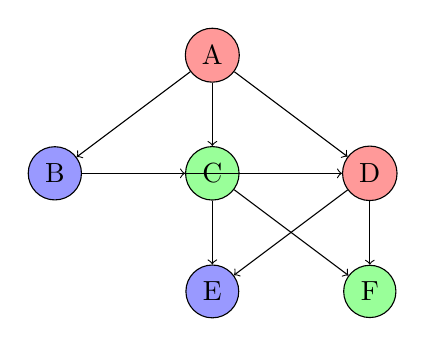
\begin{tikzpicture}
            \node[circle,draw=black,fill=red!40] (A) at (0,0) {A};
            \node[circle,draw=black,fill=blue!40] (B) at (-2,-1.5) {B};
            \node[circle,draw=black,fill=green!40] (C) at (0,-1.5) {C};
            \node[circle,draw=black,fill=red!40] (D) at (2,-1.5) {D};
            \node[circle,draw=black,fill=blue!40] (E) at (0,-3) {E};
            \node[circle,draw=black,fill=green!40] (F) at (2,-3) {F};

            \draw[->] (A) -- (B);
            \draw[->] (A) -- (C);
            \draw[->] (A) -- (D);
            \draw[->] (B) -- (C);
            \draw[->] (B) -- (D);
            \draw[->] (C) -- (E);
            \draw[->] (C) -- (F);
            \draw[->] (D) -- (E);
            \draw[->] (D) -- (F);
        \end{tikzpicture}
    \end{center}
\end{figure}

Ad esempio, dato un grafo, trovare il numero di vertici per rendere il grafo
aciclico.

\subsubsection{Proposta 1: Feedback Vertex Number}
\textbf{Feedback Vertex Number}
\begin{figure}[H]
    \centering
    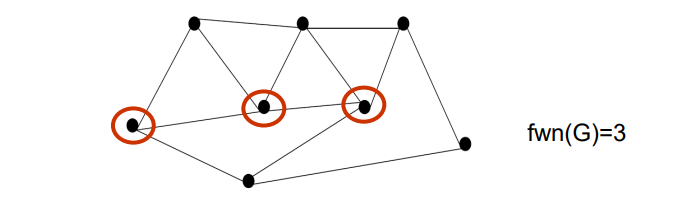
\includegraphics[width=0.7\linewidth]{chapters/images/fixed k.png}
    \caption{Feedback Vertex Number}
    \label{fig:2}
\end{figure}

In questo caso $k$ è fissato.

Ma effettivamente, \textbf{è una buona misura} quella di calcoalre quanti
vertici rimuovere come \textbf{grado di aciclicità}?

\begin{itemize}
    \item Pro: Per $k$ fissato, possiamo controllare in tempo quadratico $fwn(G) = k$
    \item \textbf{Contro}: Grafi semplici possono avere valori FVN grandi
\end{itemize}

\subsubsection{Proposta 2: Feedback Edge Number}
Una misura che ci dice \textbf{quanti archi rimuovere per rendere il grafo
    aciclico}.

A quanto pare, il problema rimane lo stesso.

\begin{figure}[H]
    \centering
    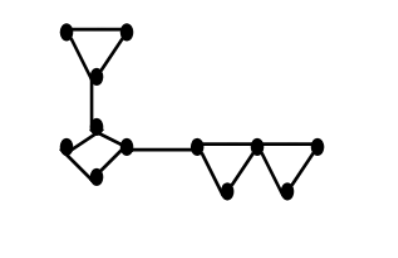
\includegraphics[width=0.7\linewidth]{chapters/images/feg.png}
    \caption{Feedback Edge Number}
    \label{fig:3}
\end{figure}

La soluzione a questi problemi è quella di \textbf{gruppare} i componenti e
creare un cluster.

\subsubsection{Biconnected Width}

\begin{definition}(Biconnected Component)
    Una componente biconnessa è un sottografo massimale che non contiene \textbf{punti di articolazione}, cioè
    un grafo che rimane connesso se rimuovo un nodo del grafo.
\end{definition}

\begin{figure}
    \centering
    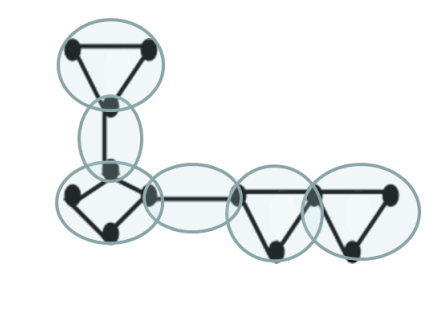
\includegraphics[width=0.7\linewidth]{chapters/images/biconnected.png}
    \caption{Biconnected Component}
    \label{fig:4}
\end{figure}

\begin{itemize}
    \item Pro: bcg(G) può essere calcolato in tempo lineare
    \item \textbf{Contro}: Aggiungere un \textbf{singolo arco} ha un effetto tremendo al bcw(g)
\end{itemize}

\subsubsection{Deep dive nella tree decomposition}

%metti 2 figure sulla stessa riga, g1.png g2.png
\begin{figure}[H]
    \centering
    \begin{minipage}[b]{0.45\linewidth}
        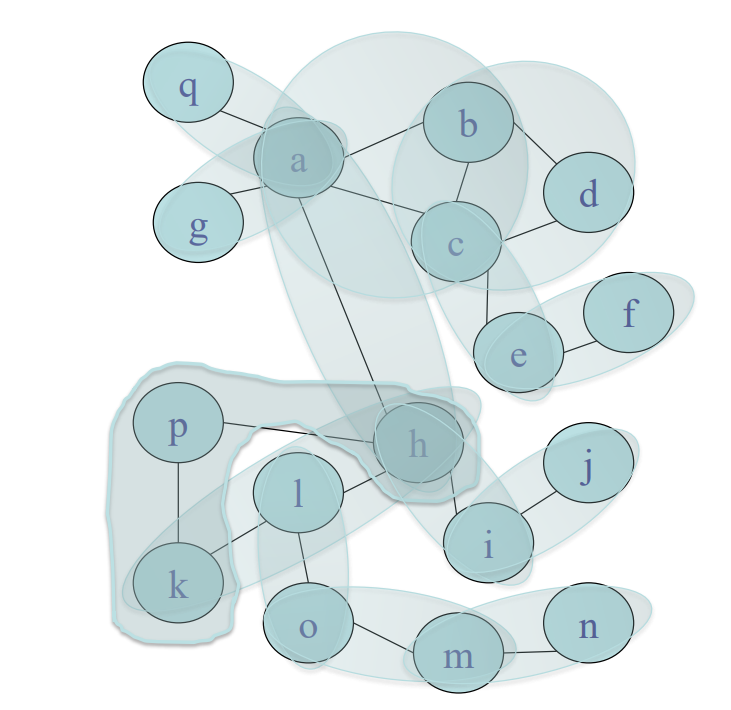
\includegraphics[width=\linewidth]{chapters/images/g1.png}
        \caption{Grafo G1}
        \label{fig:5}
    \end{minipage}
    \hspace{0.5cm}
    \begin{minipage}[b]{0.45\linewidth}
        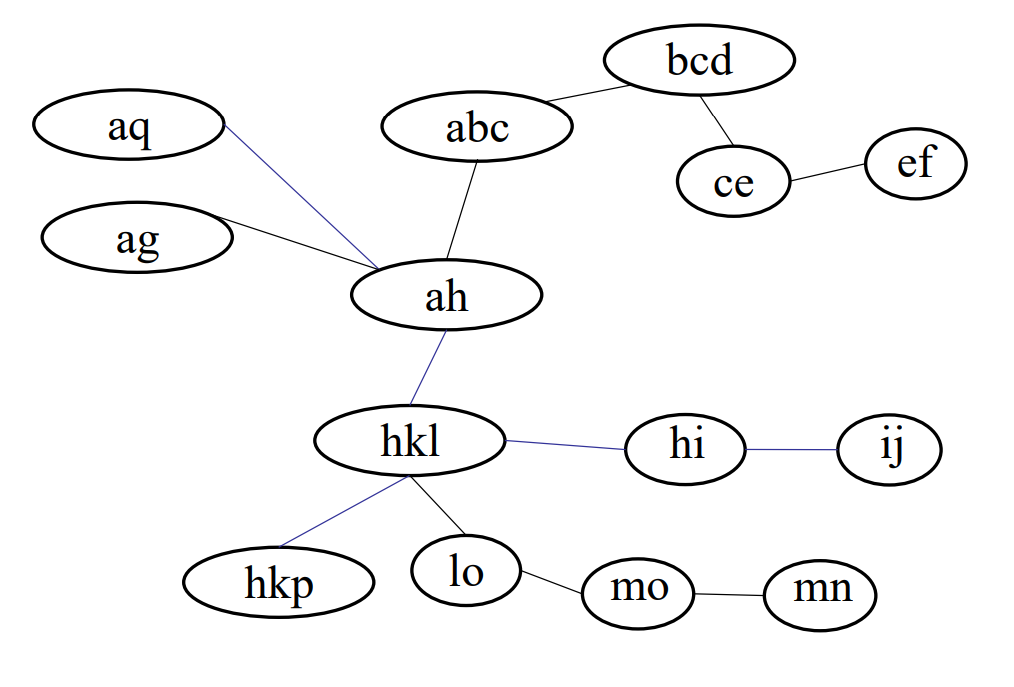
\includegraphics[width=\linewidth]{chapters/images/g2.png}
        \caption{Grafo G2}
        \label{fig:6}
    \end{minipage}
\end{figure}

Entrambe sono la stessa cosa, ma la prima è più \textbf{compatta} della
seconda. La seconda è più \textbf{esplicita}.

\begin{figure}[H]
    \centering
    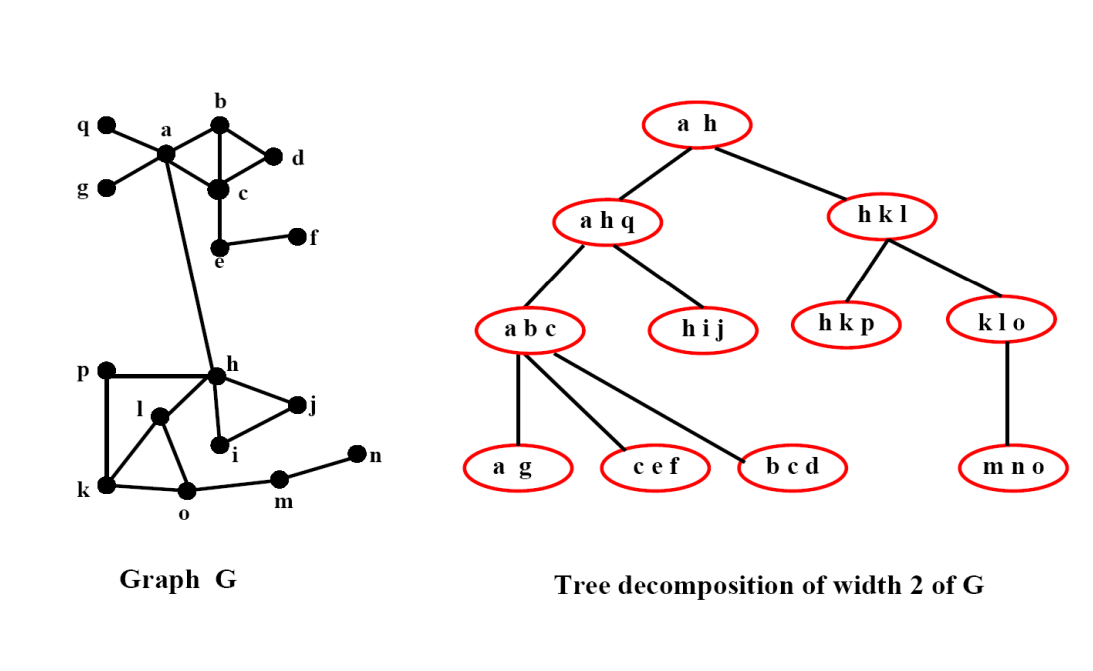
\includegraphics[width=0.7\linewidth]{chapters/images/td.png}
    \caption{Tree Decomposition con width 2}
    \label{fig:7}
\end{figure}

Praticamente, per ogni nodo, si crea un \textbf{bag} che contiene i nodi d
\textbf{vicini} e i nodi \textbf{figli}.

Quali sono le proprietà da rispettare?
\begin{itemize}
    \item Ogni arco deve essere \textbf{coperto}
    \item Se prendo un vertice qualsiasi, il sotto grafo deve rimanere connesso
\end{itemize}
\begin{figure}[H]
    \centering
    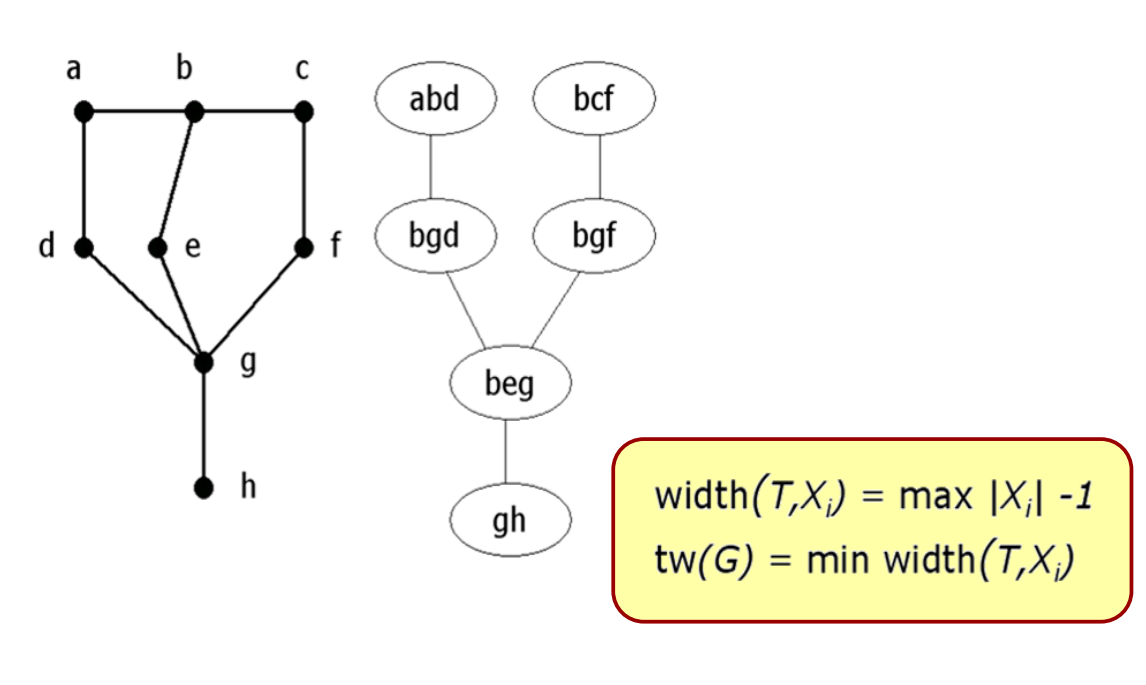
\includegraphics[width=0.7\linewidth]{chapters/images/td2.png}
    \caption{Tree Decomposition con width 2}
    \label{fig:8}
\end{figure}

In questo caso di figura \ref{fig:8} le proprietà sono rispettate!

\textbf{Tree width:} \textit{min width} su tutte le possibili composizioni.
\begin{figure}[H]
    \centering
    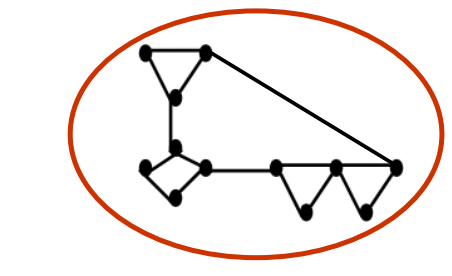
\includegraphics[width=0.7\linewidth]{chapters/images/casostrano.png}
    \caption{Tree Width in caso particolare}
    \label{fig:9}
\end{figure}

In questo caso, cerchiamo di capire come calcolare la \textit{ tree width}.

%abc
%|
%v
%cd
%|
%v
%def
%|
%v
%efg -> fg -> hij -> ikl -> bk

%Fai un grafo con questo

%bk viola la componente biconnessa e devo aggiungerela a tutti i nodi

%abc
%|
%v
%cdb
%|
%v
%defb
%|
%v
%efgb -> fgb -> hijb -> iklb -> bk

%In questo caso, il valore della width è 3

Ma possiamo ottenere un valore migliore? Possiamo ottenere 2?

%abc
%|
%v
%cdb
%|
%v
%dfb
%/   \
%v     v
%dfg   fhb -> hib -> ikb -> bk
%dge           |       | 
% v       v
%hij     ikl

La risposta è \textbf{si}, con questa configurazione posso ottenere una width
di $2$.

Le domande sono 2 ora: \textbf{Come si calcola una decomposizione?} e l'altra è
\textbf{Quando ho una decomposizione, come si risolve un problema NP-Hard?}

\begin{corollary}(Correlazoine NP-Hard e Tree Width)
    Tutti i problemi NP-Hard $2^n \rightarrow 2^k$, cioè avendo $k$ = \textbf{tree width}, i problemi NP-Hard sono risolvibili in tempo $2^k$.
\end{corollary}

\subsubsection{Robber and Cops Game}

\begin{definition}
    Il gioco Robber and Cops è un gioco dove un \textbf{Robber} deve essere catturato da un gruppo di \textbf{Cops}, e
    i Cops possono bloccare le strade per catturare il Robber.

    \begin{itemize}
        \item Input: Un grafo $G$ e un intero $k$
    \end{itemize}
\end{definition}

%2x2 con figure cop1,cop2,cop3,cop4
\begin{figure}[H]
    \centering
    \begin{minipage}[b]{0.45\linewidth}
        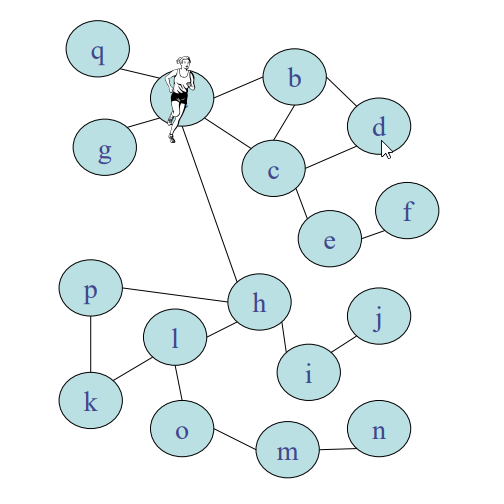
\includegraphics[width=\linewidth]{chapters/images/cop1.png}
        \caption{Cop1}
        \label{fig:5}
    \end{minipage}
    \hspace{0.5cm}
    \begin{minipage}[b]{0.45\linewidth}
        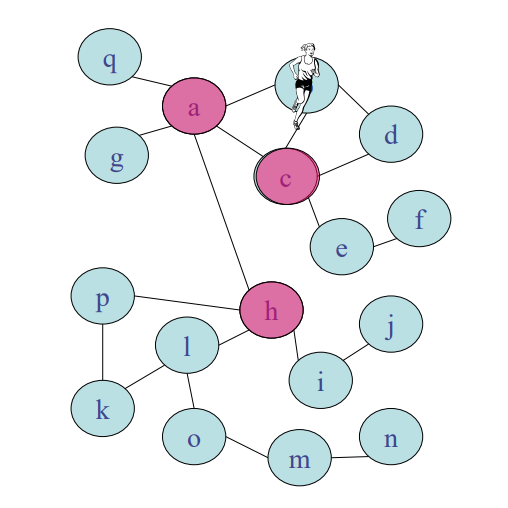
\includegraphics[width=\linewidth]{chapters/images/cop2.png}
        \caption{Cop2}
        \label{fig:6}
    \end{minipage}
\end{figure}

\begin{figure}[H]
    \centering
    \begin{minipage}[b]{0.45\linewidth}
        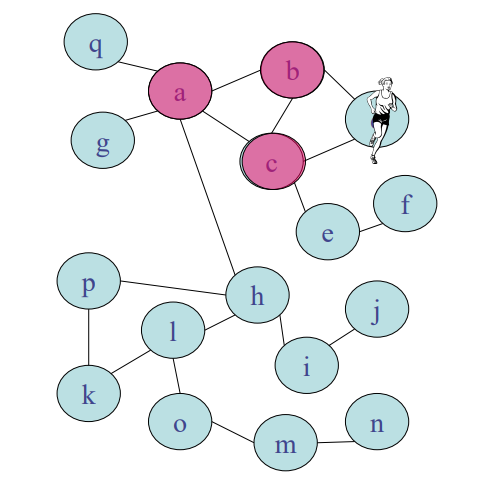
\includegraphics[width=\linewidth]{chapters/images/cop3.png}
        \caption{Cop3}
        \label{fig:5}
    \end{minipage}
    \hspace{0.5cm}
    \begin{minipage}[b]{0.45\linewidth}
        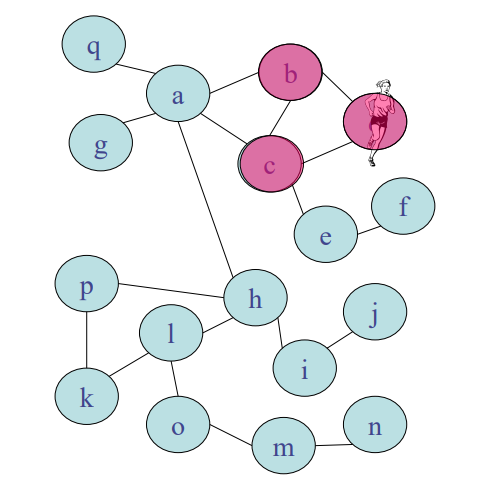
\includegraphics[width=\linewidth]{chapters/images/cop4.png}
        \caption{Cop4}
        \label{fig:6}
    \end{minipage}
\end{figure}

Cosa capiamo da questo? Che cercare di \textbf{vedere le possibili mosse} da
fare per bloccare un ladro nel grafo, praticamente ci tira fuori una
\textbf{struttura} che è una \textbf{tree decomposition.}

\textbf{Nota}: quante combinazioni di stati iniziali ci sono?
\[
    n^k
\]
dove $n$ è il numero di nodi e $k$ è il numero di poliziotti.

\textbf{Nota 2:} Il caso peggiore per una tree decomposition è la \textbf{cricca}.

\begin{definition}(Cricca)
    Una cricca è un sottografo completo, cioè un grafo in cui ogni nodo è collegato a tutti gli altri nodi.
\end{definition}

Un approfondimento algoritmico sulla \textbf{tree decomposition} dovrebbe
essere disponibile alla lezione di \textbf{laboratorio} \ref{MCnets}.

\subsubsection{3 Colorabiltà con Tree Decomposition}

Abbiamo un albero con questi nodi:
\begin{itemize}
    \item yp
    \item yzv
    \begin{itemize}
        \item zvw
        \item vz
    \end{itemize}
\end{itemize}

%fai un albero con questi nodi

Per ogni nodo, prende esattamente $3^k$ per risolvere la 3 colorabilità.

\begin{itemize}
    \item yp:
    \item \begin{itemize}
              \item RB
              \item RG
              \item BG
              \item BR
              \item GR
              \item GB
          \end{itemize}
    \item yzv:
          \begin{itemize}
              \item RBG
              \item RGB
              \item BRG
              \item BGR
              \item GRB
              \item GBR
          \end{itemize}
    \item zvw:
          \begin{itemize}
              \item RBG
              \item RGB
              \item BRG
              \item BGR
              \item GRB
              \item GBR
          \end{itemize}
    \item vz:
          \begin{itemize}
              \item \begin{itemize}
                        \item RB
                        \item RG
                        \item BG
                        \item BR
                        \item GR
                        \item GB
                    \end{itemize}
          \end{itemize}
\end{itemize}

Dove vuole arrivare? Vuole dire che se calcoli le soluzioni per i sotto problemi, si nota che ci sono delle soluzioni che vanno bene anche per alcuni problemi 
più grandi. Quindi si calcolano le \textbf{soluzioni locali} che sono $2^k$ e si utilizzano queste soluzioni per risolvere gli altri. E' quindi praticamente 
un \textbf{algoritmo di programmazione dinamica}.
\newpage

\section{Reti Neurali Convoluzionali Pre-allenate}

\textbf{Motivazione principale:} E' quello di ridurre il modello e riutilizzarlo in altri contesti, senza dover effettuare ancora un allenamento della rete.

Prendiamo l'esempio di \textbf{VCG-16} che è una rete allenata su un dataset di
immagini di una vecchia competizione. La cosa da capire è che quando vogliamo
utilizzare la rete \textbf{bisogna preparare l'input} per essere inserito nella
rete. Ad esempio, le immagini sono in $224x224$.

\begin{lstlisting}[language=Python]
# prebuild model with pre-trained weights on imagenet
model = VGG16(weights='imagenet'
, include_top=True)
model.compile(optimizer='sgd'
, loss='categorical_crossentropy')

# resize into VGG16 trained images' format
# add a dummy iniziatl axis
im = cv2.resize(img, (224, 224))
plt.imshow(im)
im = np.expand_dims(im, axis=0)
im.astype(np.float32)
print(im.shape)
\end{lstlisting}

\begin{domanda}(Come usiamo la rete?)
\end{domanda}

Se volessimo, ad esempio, classificare \textit{modelli di laptop}, questa rete
può tornare utile nella classificazione? Come facciamo? La risposta \textbf{non
    è banale.}

La risposta è \textbf{si}. Il nucleo della questione è quello di utilizzare
\textbf{il primo layer} della rete già allenata. Questa è l'idea principale del
\textbf{transfer learning}. La motivazione è quella che i livelli dopo i primi
sono troppo specifici per il nostro scopo, mentre i primi layer sono più
generici e sono quellli che si occupano di estrarre le features.

\subsection{Come si usa il transfer learning?}

\begin{definition}(Feature extraction)
\end{definition}
Il concetto principale è quello di \textbf{utilizzare i primi layer} della rete,
prendendo solamente l'output che si ottiene ,circa, a metà della rete. Questo
significa che per ogni immagine del nostro dataset si estraggono le
\textbf{features} e le si salvano, creando cosi un dataset alternativo formato
dalle features.

Successivamente si utilizzano queste feature nel quale viene fatto
l'allenamento, e quindi il task sarà quello di \textbf{classificare le
    features} nella task che ci interessa.

\begin{definition}(Fine Tuning)
\end{definition}

Il concetto di \textbf{fine tuning} è quello di utilizzare i primi layer della
rete regolarmente, come se fossero sempre funzionanti, e successivamente
utilizzare una nuova rete collegata con gli ultimi nodi utilizzati fino a quel
punto e allenarla con il nostro dataset. In questo caso diciamo che
\textbf{congeliamo} i primi layer della rete.

Per unire un modello con un altro, in Keras è molto semplice perché si possono
trattare i modelli come layer.

\begin{lstlisting}

    model = VGG16(weights='imagenet', include_top=True)

    new_model = Sequential()
    new_model.add(model)
    new_model.add(Dense(2, activation='softmax'))

    new_model.compile(optimizer='sgd', loss='categorical_crossentropy')

\end{lstlisting}
In Keras, un modello può essere congelato impostando il parametro
\textbf{trainable} su \textbf{False}.

\begin{lstlisting}[language=Python]
    model.trainable = False
\end{lstlisting}

\newpage

\section{Oltre il modello sequenziale}

Il modello sequenziale in Keras è un'implementazione semplice e intuitiva di
una rete neurale, ma ha dei limiti in termini di flessibilità e complessità. In
particolare, il modello sequenziale è limitato a reti neurali feedforward,
ovvero reti neurali in cui l'informazione fluisce in una sola direzione, senza
cicli o connessioni ricorrenti.

Ci sono molti problemi di deep learning che richiedono reti neurali più
complesse, come ad esempio le reti neurali convoluzionali per l'elaborazione di
immagini o le reti neurali ricorrenti per l'elaborazione di sequenze. In questi
casi, il modello sequenziale può essere troppo limitato per modellare
efficacemente i dati.

Inoltre, il modello sequenziale non supporta la condivisione di pesi tra i
layer, il che può essere un'importante tecnica di regolarizzazione e può
aiutare a ridurre il numero di parametri del modello. Infine, il modello
sequenziale non supporta la definizione di grafi di calcolo arbitrari, il che
può essere necessario per alcune applicazioni avanzate di deep learning.

Un'alternativa è quella del \textbf{multi input}.

\subsection{Multi input e multi output}

Quando abbiamo più input, non possiamo utilizzare il modello sequenziale. Ad
esempio, abbiamo dati eterogenei che hanno bisogno di essere elaborati in modi
diversi tra loro. Ci possono essere vari approcci che permettono di gestire
questi casi:

\begin{itemize}
    \item Il merging dei moduli, quando più input che sono eterogenei
    \item Concatenate, quando gli input sono omogenei
    \item Multiple Output: In questo caso abbiamo un solo input ma più output, e quindi
          ci saranno regressori diversi in base alla feature da predire.
    \item Inception: L'architettura a inception è una rete neurale convoluzionale
          profonda che è stata introdotta per la prima volta nel 2014. L'idea principale
          è quella di utilizzare filtri di dimensioni diverse per estrarre le features e
          poi \textbf{concatenare} le features estratte per avere un output finale.
    \item Residual: E' un archiettura che sfrutta il concetto di \textbf{residual
              learning}, ovvero l'idea di aggiungere un layer che è un'identità rispetto
          all'input.
\end{itemize}

\subsection{Functional API}

Se ci pensiamo, un modello è un qualcosa che \textit{prende in input qualcosa}
e ritorna fuori \textit{un output}. Concettualmente, è la stessa cosa di una
\textbf{funzione}. Possiamo, quindi, considerare dei moduli come delle
funzioni.

\begin{equation}
    \begin{aligned}
        \mathcal{O}_1 = M_1(I_1)                        \\
        \mathcal{O}_2 = M_2(I_2)                        \\
        \mathcal{O}_3 = Q(\mathcal{O}_1, \mathcal{O}_2) \\
    \end{aligned}
\end{equation}

dove $Q$ è una funzione che prende in input due moduli e ritorna un output.

Vediamo un esempio di come funzionano e come usare queste \textit{functional
    API}

\begin{esempio}(Functional API)
\end{esempio}

\begin{lstlisting}[language=Python]

#Vogliamo avere questa rete 
# (input: 784-dimensional vectors)
# [Dense (64 units, relu activation)]
# [Dense (64 units, relu activation)]
# [Dense (10 units, softmax activation)]
# (output: logits of a probability distribution over 10 classes)
    
inputs = keras.Input(shape=(784,))

# Qui, invece di sequenzializzare i layer, li colleghiamo
dense = layers.Dense(64, activation="relu")
x = dense(inputs)

#Abbiamo passato l'input a questo layer e otteniamo x come output
#Aggiungiamo altri layer alla rete

x = layers.Dense(64, activation="relu")(x)
outputs = layers.Dense(10)(x)

#Possiamo specificare, ora, il modello 
model = keras.Model(inputs=inputs, outputs=outputs, name="Modello funzionale")
\end{lstlisting}

\textbf{Nota:} In questo momento stiamo solamende creando la struttura
della rete, ma non stiamo ancora definendo i pesi.

\newpage

\section{Adanvced Keras}

\subsection{Subclassing}

\begin{definition}(Subclassing)
\end{definition}

Il subclassing in Keras è una tecnica avanzata per la creazione di modelli di
deep learning personalizzati. Consiste nell'estendere la classe
"tf.keras.Model" e definire il modello all'interno del metodo "init" e il
passaggio in avanti all'interno del metodo "call". In questo modo, è possibile
creare modelli di deep learning altamente personalizzati e flessibili, con la
possibilità di definire qualsiasi tipo di struttura di rete e di utilizzare
qualsiasi tipo di operazione di calcolo.

In soldoni, il subclassing ci permette di definire:
\begin{itemize}
    \item Loss personalizzate
    \item Layer personalizzati
    \item Metriche personalizzate
    \item Modelli personalizzati
\end{itemize}

Chiaramente questo aumenta la complessità del codice, ma aumenta la
flessibilità e la possibilità di avere un controllo maggiore di quello che ci
fornisce di base Keras.

Ad esempio nelle \textbf{Generative Adversarial Networks - GAN} il concetto di
training viene fatto in modo diverso, poiché non si usa la \textbf{stochastic
    gradient descent}. Nelle GAN anche l'ordine di apprendimento delle reti è
importante; allenare contemporaneamente potrebbe portare a risultati strani e
non convenienti. Ci sono tecniche e scenari specifici che hanno apprendimenti
anch'essi specifici. Ovviamente, come detto prima, aumenta la complessità ma
aumenta anche la flessibilità.

\newpage


\section{Serie Temporali | Time Series}
\label{sec:time-series}

Le serie temporali vengono usate in campi come la \textbf{predizione di prezzi
    di azioni}, che richiedono una conoscenza dei trend passati per funzionare. Le
reti neurali Feed Forward non considerano gli stati temporali. Si utilizza,
infatti, un'altra architettura di rete neurale: \textbf{Recurrent Network -
    RNN}

\subsection{Recurrent Neural Network RNN}

Una RNN itera sugli elementi mantenendo uno stato che contiene informazioni di
ciò che è stato visto finora. Questo stato viene passato avanti ad ogni
iterazione.

\begin{definition} RNN

\end{definition}

Una RNN è un grafo con cicli. I percettroni beneficiano del feedback dei loop.
L'output di un percettrone al tempo $t$ è coinvolto nel calcolo dell'output di
un percettrone al tempo $t+1$.

%figura da fare
\begin{figure}[H]
    \begin{center}
        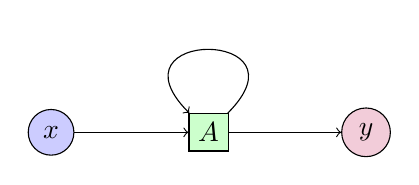
\begin{tikzpicture}
            \node[fill=blue!20, draw,circle] (x) at (0,0) {$x$};
            \node[fill=green!20, draw,rectangle] (A) at (2,0) {$A$};
            \node[fill=purple!20, draw,circle] (y) at (4,0) {$y$};
            \draw[->] (x) -- (A);
            \draw[->] (A) -- (y);
            \draw[->] (A) to [out=45,in=135,looseness=8] (A);
        \end{tikzpicture}
    \end{center}
    \caption{RNN}
\end{figure}

%figura da fare
\begin{figure}[H]
    \begin{center}
        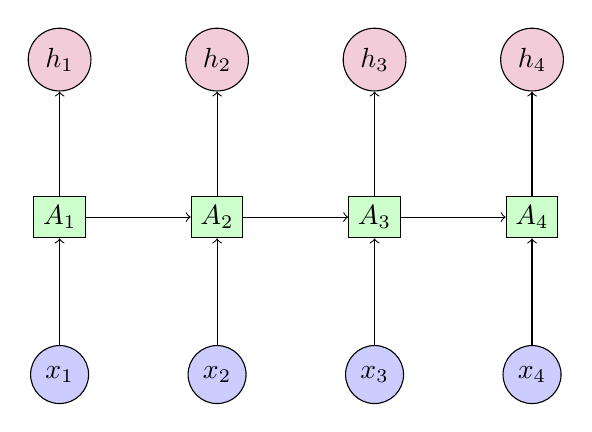
\begin{tikzpicture}
            \node[fill=blue!20, draw,circle] (x_1) at (0,0) {$x_1$};
            \node[fill=green!20, draw,rectangle] (A_1) at (0,2) {$A_1$};
            \node[fill=purple!20,draw,circle] (y_1) at (0,4) {$h_1$};

            \node[fill=blue!20, draw,circle] (x_2) at (2,0) {$x_2$};
            \node[fill=green!20, draw,rectangle] (A_2) at (2,2) {$A_2$};
            \node[fill=purple!20,draw,circle] (y_2) at (2,4) {$h_2$};

            \node[fill=blue!20, draw,circle] (x_3) at (4,0) {$x_3$};
            \node[fill=green!20, draw,rectangle] (A_3) at (4,2) {$A_3$};
            \node[fill=purple!20,draw,circle] (y_3) at (4,4) {$h_3$};

            \node[fill=blue!20, draw,circle] (x_4) at (6,0) {$x_4$};
            \node[fill=green!20, draw,rectangle] (A_4) at (6,2) {$A_4$};
            \node[fill=purple!20,draw,circle] (y_4) at (6,4) {$h_4$};

            \draw[->] (x_1) -- (A_1);
            \draw[->] (A_1) -- (y_1);

            \draw[->] (x_2) -- (A_2);
            \draw[->] (A_2) -- (y_2);

            \draw[->] (x_3) -- (A_3);
            \draw[->] (A_3) -- (y_3);

            \draw[->] (x_4) -- (A_4);
            \draw[->] (A_4) -- (y_4);

            \draw[->] (A_1) -- (A_2);
            \draw[->] (A_2) -- (A_3);
            \draw[->] (A_3) -- (A_4);
        \end{tikzpicture}
    \end{center}
    \caption{Unfolded RNN}
\end{figure}

\textbf{Ci sono 2 equazioni da tenere a mente}:

\textbf{Rete Elman:}
\begin{equation}
    \begin{aligned}
        h_t = \sigma(W_h x_t + U_h \textcolor{green}{h_{t-1}}+b_h) \\
        y_t = \sigma(W_y h_t + b_y)
    \end{aligned}
\end{equation}

\textbf{Rete Jordan:}
\begin{equation}
    \begin{aligned}
        h_t = \sigma(W_h x_t + U_h \textcolor{purple}{y_{t-1}}+b_h) \\
        y_t = \sigma(W_y h_t + b_y)
    \end{aligned}
\end{equation}

Dove:
\begin{itemize}
    \item $x_t$ = Vettore di input
    \item $y_t$ = Vettore di output
    \item $h_t$ = Vettore di layer nascosto
    \item $W,U,b$ = Pesi e Bias
    \item $\sigma_h, \sigma_y$ = Funzioni di attivazione
\end{itemize}

%inserisci foto
\begin{figure}
    \begin{center}
        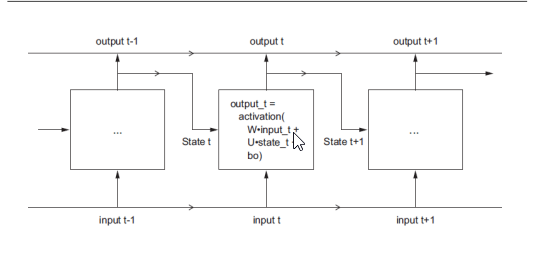
\includegraphics[scale=0.8]{images/RNN.png}
    \end{center}
    \caption{RNN}
\end{figure}

\subsubsection{L'utilizzo delle RNN}

Alla fine, tutto ciò che noi andiamo a fare è \textbf{aggiungere dei layer}
alla nostra rete.

\begin{lstlisting}[language=python]
    model.add(SimpleRNN(32, return_sequences=True))#Return a list
    model.add(SimpleRNN(32, return_sequences=True))#Return a list
    model.add(SimpleRNN(32, return_sequences=True))#Return a list
    model.add(SimpleRNN(32)) # last layer only returns last output

    model.summary()
\end{lstlisting}

Un esempio di codice di rete è:

\begin{lstlisting}[language=python]
from keras.datasets import imdb
from keras.preprocessing import sequence

max_features = 10000 # number of words to consider as features
maxlen = 500
batch_size = 32

(input_train, y_train), (input_test, y_test) = imdb.load_data(num_words=max_features)

input_train = sequence.pad_sequences(input_train, maxlen=maxlen)
input_test = sequence.pad_sequences(input_test, maxlen=maxlen)

from keras.layers import Dense

model = Sequential()
model.add(Embedding(max_features, 32))
model.add(SimpleRNN(16))
model.add(Dense(1, activation='sigmoid'))
model.compile(optimizer='rmsprop'
            , loss='binary_crossentropy'
            , metrics=['acc'])

history = model.fit(input_train, y_train,
            epochs=10,
            batch_size=128,
            validation_split=0.2)
\end{lstlisting}

Questo codice ha un problema: \textbf{non funziona}. Il problema è la
\textbf{back propagation} attraverso il tempo. La normale backpropagation non
funziona e ha bisogno di un cambiamento per adattarsi al \textbf{feedback
    loop}. Immaginiamo di avere una funzione del genere:
\begin{equation}
    f(f(f(f(f(f(f(f(f(f(f(f(x_0 | x_1 , \dots , x_n))))))))))))
\end{equation}

Praticamente si ha un numero di derivate ripetuto. Poi, dalle slides, dopo
tutti i calcoli si arriva ad avere un risultato in cui la derivata ha valore
che \textbf{tende sempre a 0}. Come se si trovasse sempre un minimo globale.
Quindi, questo approccio non funziona. Il \textbf{gradiente sparisce}

\textbf{Motivazione:} la sequenza è troppo lunga.
\begin{definition}(
    Spiegazione del problema )

    Il problema della dipendenza a lungo termine è una sfida nell'addestramento
    delle reti neurali artificiali, in particolare le reti neurali ricorrenti
    (RNN). Si riferisce alla difficoltà che queste reti hanno nell'apprendere a
    collegare informazioni o contesti da passaggi precedenti nella sequenza a
    passaggi successivi.

    Ad esempio, considera un modello di linguaggio che cerca di prevedere la parola
    successiva in una frase. Se la frase è "Sono cresciuto in Francia... parlo
    fluentemente ---", il modello deve ricordare il contesto della "Francia" da
    molto prima nella frase quando arriva al punto vuoto, così può riempirlo con
    "francese". Questa è una dipendenza a lungo termine.

    Le RNN fanno fatica con questo a causa del problema dei "gradienti che
    svaniscono". Durante la retropropagazione, i gradienti spesso diventano sempre
    più piccoli man mano che vengono propagati all'indietro nel tempo. Ciò
    significa che gli aggiornamenti ai pesi che collegano i passaggi precedenti
    nella sequenza a quelli successivi possono essere molto piccoli, e la rete può
    non riuscire a imparare queste dipendenze a lungo termine.
\end{definition}

Una proposta di soluzione è quella di \textbf{cambiare la funzione di
    attivazione}.

\textbf{Soluzione}: Long Short Term Memory (LSTM)

\subsection{Long Short Term Memory (LSTM)}

Queste RNN speciali sono reti capaci di risolvere il problema delle dipendenze
a lungo termine. In paticolare, sono state progettate per \textbf{controllare
    la sparizione del gradiente} e \textbf{evitare proprio il problema della
    dipendenza a lungo termine}

%inserisci foto
\begin{figure}
    \begin{center}
        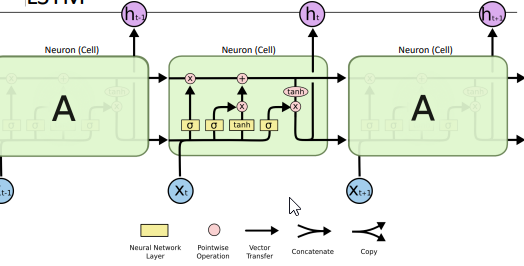
\includegraphics[scale=0.8]{images/LSTM.png}
    \end{center}
    \caption{LSTM}
\end{figure}
Riguardo l'archiettura, parliamo di una cosa importante.

\textbf{Lo stato della cella} salva un'informazione interna della catena \textbf{Storico interno}. Questa informazione,
se rilevante, può essere \textbf{propagata}. Per controllare il flow di queste informazioni si una un \textbf{gate}. Servono, appunto,
per decidere quali informazioni far passare.

\textbf{Ci sono formule da ricopiare}
\begin{itemize}
    \item \textbf{Forget Gate}: decide quali informazioni scartare e quali tenere
          \[
              f_t = \sigma(W_f \cdot[h_{t-1}, x_t] + b_f)\]
          \begin{figure}[H]
              \begin{center}
                  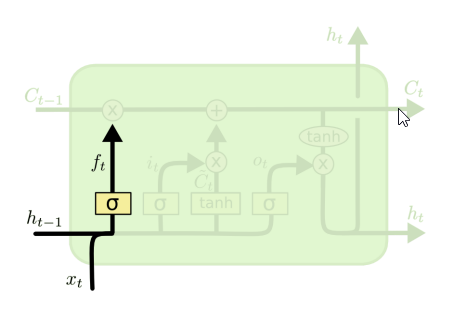
\includegraphics[scale=0.8]{images/forgetgate.png}
              \end{center}
              \caption{Forget Gate}
          \end{figure}
    \item \textbf{Input Gate}: decide quali informazioni passare e quanto devono influenzare lo storico interno
          \begin{equation}
              \begin{aligned}
                  i_t = \sigma(W_i \cdot [h_{t-1}, x_t] + b_1)       \\
                  \tilde{C}_t = tanh(W_C \cdot [h_{t-1}, x_t] + b_C) \\
              \end{aligned}
          \end{equation}
          \begin{figure}[H]
              \begin{center}
                  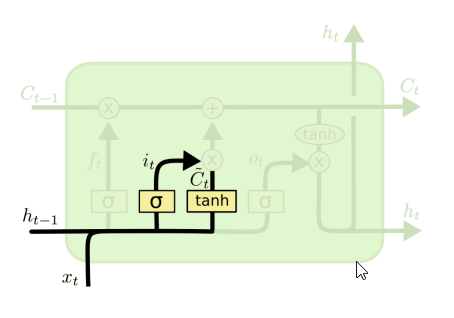
\includegraphics[scale=0.8]{images/inputgate.png}
              \end{center}
              \caption{Input Gate}
          \end{figure}
    \item \textbf{Aggiornamento dello stato interno}: Gate che risolvono il problema della dipendenza a lungo termine e del gradiente che svanisce
          \[
              C_t = f_t * C_{t-1} + i_t * \tilde{C_t}\]
          \begin{figure}[H]
              \begin{center}
                  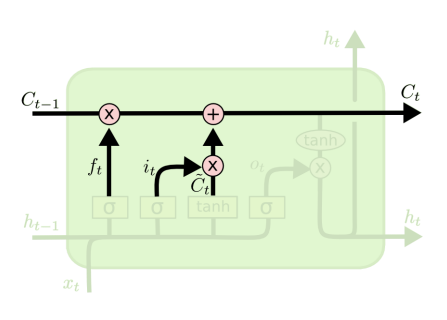
\includegraphics[scale=0.8]{images/update.png}
              \end{center}
              \caption{Update State}
          \end{figure}
    \item \textbf{Output Gate}: L'output dipende dallo stato interno della cella. La LSTM controlla quanto l'output deve essere influenzato dallo storico interno
          \begin{equation}
              \begin{aligned}
                  o_t = \sigma(W_o \cdot [h_{t-1}, x_t] + b_o) \\
                  h_t = o_t * tanh(C_t)
              \end{aligned}
          \end{equation}
          \begin{figure}[H]
              \begin{center}
                  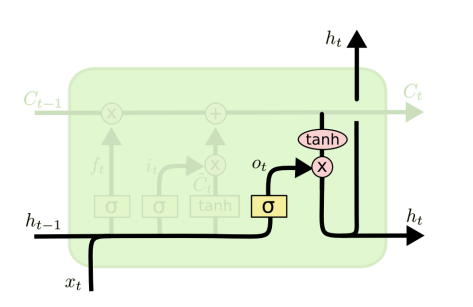
\includegraphics[scale=0.8]{images/outputgate.png}
              \end{center}
              \caption{Output Gate}
          \end{figure}

\end{itemize}

Ricordiamo che gli elementi sono:
\begin{itemize}
    \item $x_t$ = Vettore di input
    \item $y_t$ = Vettore di output
    \item $h_t$ = Vettore di layer nascosto
    \item $W,U,b$ = Pesi e Bias
    \item $\sigma_h, \sigma_y$ = Funzioni di attivazione
\end{itemize}

\begin{lstlisting}[language=python]
from keras.layers import LSTM

model = Sequential()
model.add(Embedding(max_features, 32))
model.add(LSTM(32))
model.add(Dense(1, activation='sigmoid'))
model.compile(optimizer='rmsprop'
            ,loss='binary_crossentropy'
            ,metrics=['acc'])

            history = model.fit(input_train, y_train,
epochs=10,
batch_size=128,
validation_split=0.2)
\end{lstlisting}

\newpage
\section{Autoencoders, Transformer}

Stiamo vedendo un esempio alla lavagna dove mostra come lavora un autoencoder e
che problema ha la struttura.

\textbf{La loss} è condizionata dai \textbf{vincoli di fattibilità} che ci sono. Nel senso,
si ha un valore in input \textbf{x} che si prende dai deti e lo si da in pasto all'\textbf{encoder}. Si ottiene uno
\textbf{spazio latente} che è un sottoinsieme dello spazio di input. Se prendiamo un punto nello spazio, però,
non siamo sicuri che possa \textbf{soddisfare} i vincoli che ci sono. La loss, allora, va aggiustata
tenendo conto di questo problema.

\[
    \mathcal{L}(x, \bar{x}) + \mathcal{L}_i(\bar{x})
\]

\begin{domanda}(Perché usare un autoencoder?)
    Voglio avere dei vettori che siano \textbf{rappresentativi} di quello che ho in input.
\end{domanda}

\textbf{Embedding:} Il risultato di applicare un \textbf{autoencoder} a qualcosa. Mappare \textbf{input} a \textbf{vettori}, applicando
il concetto di similarità per ottenere una semantica.

\textbf{Word Embedding}: Il risultato di costruire un latent space da un'insieme di parole.

Mappiamo le parole in \textbf{vettori}, ma non in modo generico. Vogliamo che
le parole che hanno un significato simile siano vicine nello spazio.
Probabilmente, questi punti vicini nello spazio \textbf{condividono} delle
feature tra loro. Parola chiave: \textbf{contesto} simile.

\[
    Embedding \implies Semantic
\]

\subsection{Cosa si può fare con gli autoencoder?}

Tutto ciò che si fa nel machine learning, può essere applicato a tutto quanto
con gli autoencoders.

\textbf{Feature Selection} è un problema molto generico per il \textit{machine learning}. Si ha un insieme di feature
e si vuole selezionare quelle più importanti. Come si applicano gli autoencoder in questo problema?

Qualcosa con \textbf{clustering}.

\textbf{Outlier detection | Anomaly detection}: In una distribuzione, un \textbf{outlier} è qualcosa che non rientra in questa distribuzione dei dati. Come outlier ci sono vari tipi
nel mondo reale:
\begin{itemize}
    \item Azioni strane
    \item Attacchi informatici
    \item Problemi di salute
    \item \dots
\end{itemize}

Ma la task difficile è effettivamente \textbf{come si definisce un outlier?}.
E' un concetto abbastanza complesso.

Immaginiamo di avere \textbf{3 cluster} con una nuvola di punti all'interno. Si
potrebbe calcolare una distanza dal centro e considerare i punti fuori dal
cluster come outlier. Gli autoencoder, però, risolvono questo problema in modo
più semplice.

Immaginiamio di avere $x_1, \dots, x_n$ dati. Si costruisce un autoencoder che
prende in input $x_i$ e si mappa $x_1 \rightarrow z_1, \dots, x_n \rightarrow
    z_n$. Si da in pasto al decoder e si ottiene $\bar{x_1}, \dots, \bar{x_n}$. Si
ha anche, quindi, un error $\varepsilon = ||x_i - \bar{x_i}||$. Questo errore
possiamo considerarlo come una \textbf{loss}. Maggiore sarà la loss, più
probabile è che il punto sia un outlier.

\textbf{Classification:} Consideriamo un dataset $x_1, \dots, x_n$ e alla fine vogliamo classificare con \textbf{yes} o \textbf{no} per una motivazione $m$ generica.
Si crea il latent space mappando $x_1 \rightarrow z_1, \dots, x_n \rightarrow z_n$ e si da il \textbf{latent space} in pasto ad una \textbf{feed forward network} che ritorna, appunto, \textbf{yes} o \textbf{no}.

Immaginiamo di avere delle immagini, tipo \textbf{gente che ha un cappello.}
Come facciamo a dire che le persone con il cappello siano vicine tra loro?
Magari ci saranno correlazione tra le feature, come ad esempio il colore degli
occhi, la pelle, i capelli, ecc...

Siccome il problema principale è che \textbf{non si ha controllo} su questo
problema, si utilizza un \textbf{variational autoencoder}. Lo scopo è quello di
condizionare \textbf{come vengono generati} i punti all'interno del latent
space. In pratica, \textbf{rendono lo spazio continuo}.

\[
    \mathcal{L}(x, \bar{x}) + \mathcal{L}_c(\bar{x}) + \mathcal{L}_s(E(x), FF(E(x)))
\]

dove con \textbf{E} si indica l'encoder e \textbf{FF} la feed forward network.

\textbf{Novità negli autoencoder}: Invece di costruire una funzione di loss da zero come abbiamo fatto sopra, si è cominciato ad usare un architettura diversa. L'architettura
non prende una singola unità per dataset, ma prende una \textbf{coppia} di elementi alla volta.

\begin{equation}
    \begin{aligned}
        x_1 \rightarrow E \rightarrow z_1 \rightarrow D \rightarrow \bar{x}_1 \\
        x_2 \rightarrow E \rightarrow z_2 \rightarrow D \rightarrow \bar{x}_2 \\
    \end{aligned}
\end{equation}

Alla fine qui si applica una loss diversa, calcolata in questo modo:

\[
    L(\pm d(z_1, z_2))
\]

dove $d$ è una funzione di distanza. Si vuole che la distanza tra i due punti
sia piccola se i due punti sono simili, mentre se sono diversi si vuole che sia
grande.

%grafico con 2 punti nelo spazio
\begin{figure}[H]
    \begin{center}
        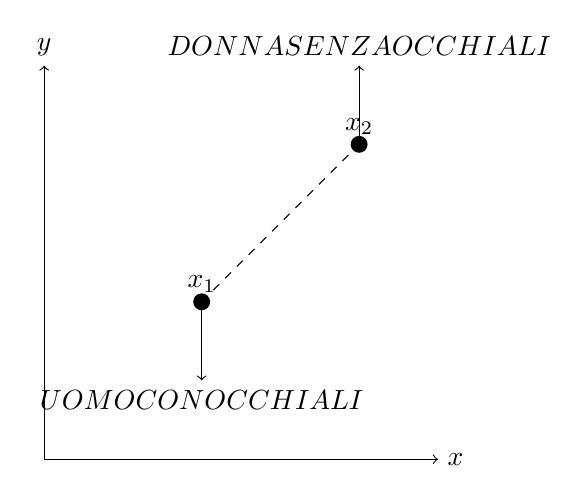
\begin{tikzpicture}
            \draw[->] (0,0) -- (5,0) node[right] {$x$};
            \draw[->] (0,0) -- (0,5) node[above] {$y$};
            \draw[fill=black] (2,2) circle (0.1) node[above] {$x_1$};
            \draw[fill=black] (4,4) circle (0.1) node[above] {$x_2$};

            %Scrivi UOMO su x1
            \draw[->] (2,2) -- (2,1) node[below] {$UOMO CON OCCHIALI$};

            %Scrivi DONNA SENZA OCCHIALI su x2 sopra
            \draw[->] (4,4) -- (4,5) node[above] {$DONNA SENZA OCCHIALI$};

            %retta che unisce i due punti
            \draw[dashed] (2,2) -- (4,4);
        \end{tikzpicture}
    \end{center}
    \caption{Esempio di spazio latente}
\end{figure}

Gli elementi che saranno sulla retta, circa, saranno elementi che avranno
feature di entrambi i punti, quindi ipoteticamente se stiamo parlando di
immagini, saranno uomini senza occhiali, donne con occhiali, ecc..., con altri
elementi che fanno parte di entrambi i punti.

\subsection{Accenno su Style Transfer}

Immaginiamo di avere 2 immagini:
\begin{itemize}
    \item Quadro
    \item Immagine normale
\end{itemize}

Diamo entrambe le immagini a 2 $Encoder$ e le uniamo in un unico $Encoder$. Si
ha un latent space e si ottiene una $Z$. \textbf{Non abbiamo un output} e va
calcolata una loss. La funzione è la seguente:
\[
    \mathcal{L}(Z, \alpha) + \mathcal{L}(Z, \beta)
\]

\subsection{Accenno su Stable Diffusion}

Assumiamo di avere un'immagine \textbf{corrotta} e sìvogliamo aggiungere
\textbf{noise random}, corrompendola. Noi sappiamo quali pixel sono quelli
corrotti.

L'architettura è \textbf{Encoder, Decoder}, la \textbf{loss} è ricostruire
\textbf{l'errore}. Vogliamo costruire \textbf{IL NOISE} che abbiamo aggiunto,
come risultato.

Si fanno degli step incrementali, aggiungendo man mano del noise all'immagine.
\textbf{Se si allena} un sistema con questa sequenza, cioè con l'immagine
chiara aggiungendo noise man mano, si \textbf{ottiene un risultato assurdo}: si
riesce a ricostruire l'immagine chiara.

\subsection{Autoencoder per le sequenze}

%immagine  dalla cartella
\begin{figure}[H]
    \centering
    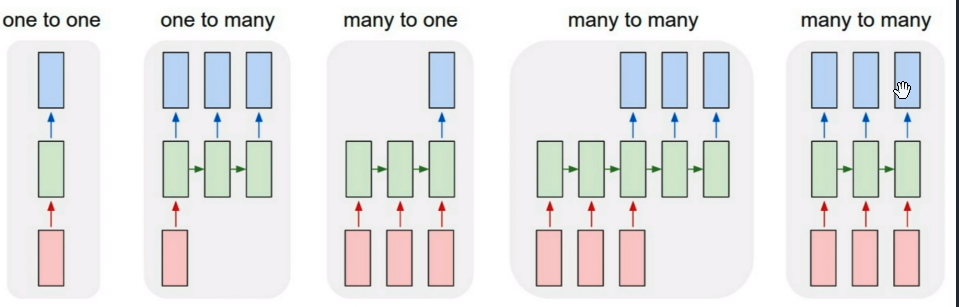
\includegraphics[width=0.8\linewidth]{images/archRNN.png}
    \caption{Autoencoder per le sequenze}
    \label{fig:seq}
\end{figure}

Queste varie architetture si utilizzano per casi d'uso particolari:

\begin{itemize}
    \item One to One: Usata per le \textbf{classification}
    \item One to Many: Viene usata per \textbf{image captioning}
    \item Many to One: Usata per la sentiment analysis
    \item Many to Many: Usata per Machine Translation
    \item Many yo Many Synched: Video classification for each frame
\end{itemize}

\begin{domanda}(Nelle many to many dov'è il latent space?)

    Il latent space nel quarto esempio è il quadrato verde dal quale comincia la
    parte di deconding
\end{domanda}

\subsubsection{Seq2Seq}
Il modello si basa su un training che non da l'output di ogni time step al prossimo, ma sono il target dello step del training. A tempo di inferenza, il decoder
da l'output di ogni time step come input al prossimo.

\textit{Definizione di Chat:} Questo è un tipo di modello utilizzato per le sequenze, come le serie temporali o 
le sequenze di parole in un testo. Il modello è composto da due parti: un encoder, che trasforma l'input in una 
rappresentazione latente, e un decoder, che genera l'output a partire dalla rappresentazione latente. Durante 
l'addestramento, l'output di ogni passo temporale non viene dato come input al passo successivo. Invece, 
l'output di ogni passo temporale è il target per l'addestramento. Durante l'inferenza, l'output di ogni
 passo temporale viene dato come input al passo successivo.

\subsubsection{Training di Seq2Seq}


\begin{itemize}
    \item \textbf{Encoder}: \textit{word2id} + \textit{embedding}: Si passa ogni token della stringa fino ad un punto in cui si fa decoding.
    \item \textbf{Decoder}: Loop in cui tra tutte le parole si prende quella con la \textbf{probabilità maggiore}. \textit{Embedding} + \textit{id2word} 
\end{itemize}

\begin{figure}[H]
    \begin{center}
        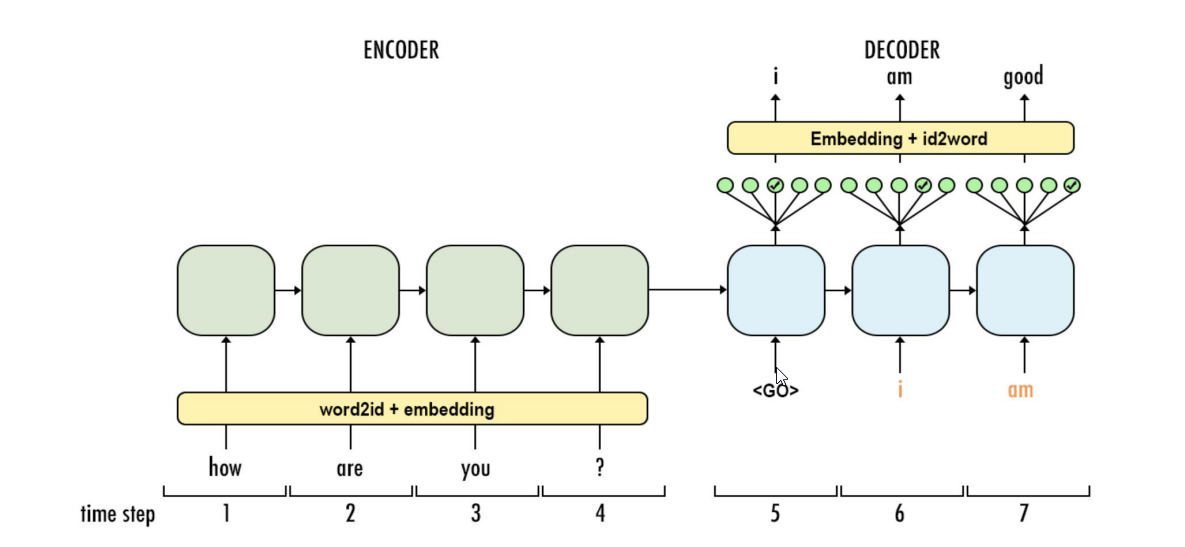
\includegraphics[width=0.8\linewidth]{images/seq2seq.png}
    \end{center}
\end{figure}


\subsubsection{Problemi di questa architettura}

Il \textbf{contesto} della frase è tutto concentrato nel primo nodo dove si inizia il decoding. Serve il concetto di \textbf{attenzione}.
Proviamo a spiegarlo con un grafico:

%disegna 4 quadrati, ogni quadrato ha un testo sotto, ogni quadrato ha un quadrato sopra

Abbiamo una frase formato da delle parole. Abbiamo un inizio dove inizia il decoding. Per processare questo, l'attenzione è basata in base al nodo di \textbf{inizio}, si passa questo valore 
alla rete neurale, si usa una \textbf{softmax} calcolata dinamicamente ogni volta che va calcolata una nuova parola, basandosi sui pesi del contesto della parola da processare.


Tocca farsela spiegare da chat più tardi e mettere una cazzo di immagine porco dio.


\subsection{Da Seq2Seq ad accenni Transformer}

\textbf{Seq2Seq} è un modello che si basa su \textbf{RNN} e \textbf{LSTM}. Questi modelli hanno un problema: \textbf{sono lenti}. Per ogni parola, si deve aspettare che la rete neurale
faccia il suo lavoro. Non solo. Ciò che viene calcolato per le celle, rimane li. Non si può eliminare.

Il Paper \textit{Attention is All You Need} ha cambiato il mondo del NLP. Il modello si basa su \textbf{Transformer}. L'architettura ha le seguenti caratteristiche:
\begin{itemize}
    \item Nell'Encoding il testo è salvato in un vettore 
    \item Le parole sono processate con \textbf{Word Embedding}
    \item Il meccanismo di \textbf{attenzione} è il core di questa architettura
\end{itemize}

\begin{figure}[H]
    \begin{center}
        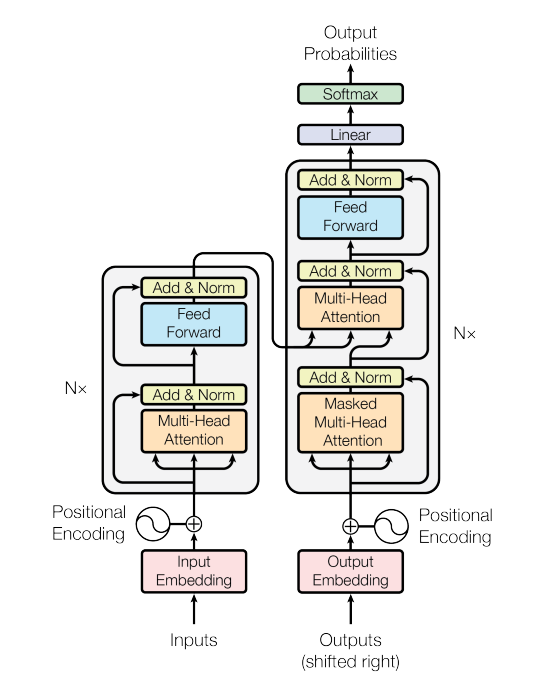
\includegraphics[width=0.8\linewidth]{images/transformer.png}
    \end{center}
    \caption{Architettura di Transformer}
\end{figure}

Spacchiamo l'input in pezzi:

\textbf{Input Embedding}: Si fa un embedding \textbf{parola per parola}.

Successivamente si ha un \textbf{positional encoding}: Ci serve mantenere l'informazione dell'\textit{ordine} delle parole. Per farlo, basta semplicemente 
avere una coppia (Indice, Parola Embeddata).

Si ha un \textbf{Multi-head Attention}: Serve per calcolare l'attenzione tra le parole. Si calcola l'attenzione tra le parole e si calcola la \textbf{query}.
Il valore viene passato ad una \textbf{Feed Forward Network}. Si ripete il processo, passando il risultato della \textbf{Feed Forward Network} alla \textbf{Multi-head Attention}, che 
successivamente ripassa il risultato alla \textbf{Feed Forward Network}, poi ad un \textbf{linear layer} e infine ad un \textbf{softmax}. Il risultato è un \textbf{vettore di probabilità}.

\textbf{Output Embedding}: E' il vettore delle frasi nella lingua da tradurre, anche questa con un positoinal encoding. Si passa questo ad una \textbf{masked multihead attention}, che vedremo poi come funziona, e che poi si collega alla \textbf{Multi-head attention} alla quale 
si era passata la prima \textbf{Feed Forward}.

Si utilizza questa struttura \textbf{shiftata a destra}; questo è il trick per sapere tutto l'input che si ha a disposizione della frase da tradurre e solamente la posizione della parola fino a quel punto.
per fare in modo che la rete possa farlo in un colpo solo, cioè il task per fare una predizione della frase di output in un colpo solo. 


Sommario: 
\begin{itemize}
    \item Input: la stringa
    \item Output: la stringa tradotta shiftata di uno a destra
    \item Se ho la frase: oggi sono qui, con posizione: 
    \begin{itemize}
        \item 0: oggi
        \item 1: sono
        \item 2: qui
    \end{itemize}
    \item Se mentre traduco sono alla posizione 2:
    \begin{itemize}
        \item 0: $\_$
        \item 1: oggi
        \item 2: sono
    \end{itemize}
    \item Ho la conoscenza fino alla posizione 2, e a runtime produco la stringa basandoci sulle probabilità che ho calcolato
\end{itemize}

\subsubsection{Cosa significa Masking?}

Come hanno fatto ad allenare CHAT-GPT? Quali sono stati gli \textbf{input, output}? Su cosa? A quali domande risponde? Come funziona? La risposta è nel \textbf{masking}.

Il concetto è quello di \textbf{aggiungere noise alle parole}, come in diffusion. ChatGPT ha imparato a rimuovere 
il noise dalle parole, ed è praticamente stato usato come un noise remover. In questo modo, la rete ha imparato.

\newpage

\section{Architettura Transformer}

\begin{figure}[H]
    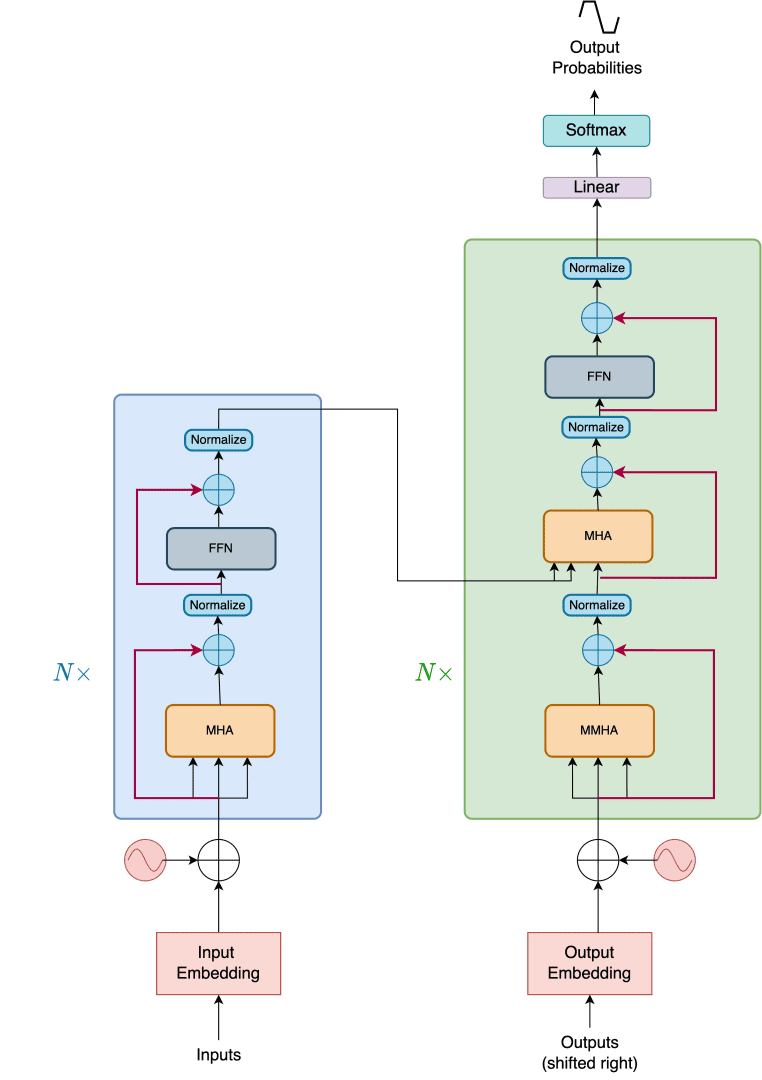
\includegraphics[width=\textwidth]{images/entire-architecture.png}
    \caption{Architettura Transformer}
\end{figure}

\begin{definition}(Attention)
    L'Attention è un meccanismo che assegna un peso a
    ogni parte dell'input durante il processo di elaborazione
    di un modello Transformer. Questi pesi determinano quanto ogni
    parte dell'input contribuisce all'output. Matematicamente,
    l'Attention può essere definita come una funzione $f$ che
    prende in input una query $q$, un insieme di coppie chiave-valore
    $(k, v)$, e restituisce un output $o$ calcolato come una somma pesata dei valori
    $v$, dove i pesi sono determinati dalla compatibilità tra la query $q$ e
    le chiavi $k$.
\end{definition}

\subsection{Multihead Attention}

\begin{figure}[H]
    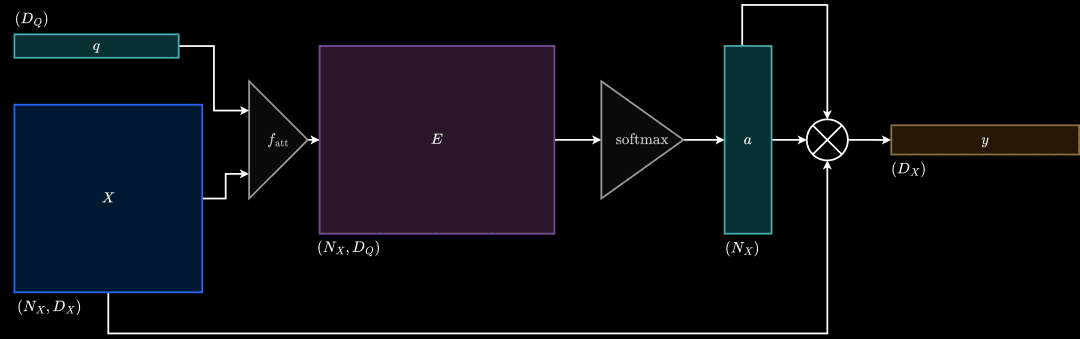
\includegraphics[width=\textwidth]{images/evolution-Version-0.png}
    \caption{Multihead Attention Versione 0}
\end{figure}

\textbf{fatt}: F-attention è la rete dove ci sono i parametri che vanno allenati per questa architettura. Tutto quanto
risiede in questo punto.

Ma ci sono state altre versioni per questa architettura. La versione 0 è quella
che abbiamo visto prima. La versione 1 è praticamente una versione che ha $D_Q$
fissato. Sparisce la \textbf{fatt} e quindi sparisce la rete neurale in questa
architettura.

\begin{figure}[H]
    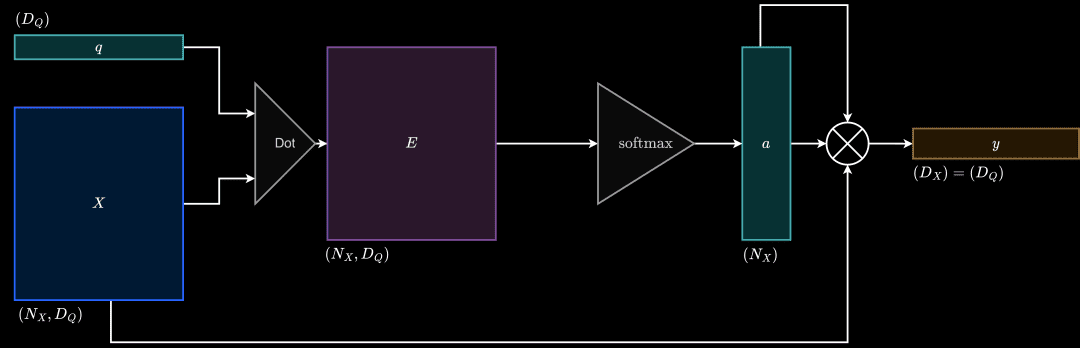
\includegraphics[width=\textwidth]{images/evolution-Version-1.png}
    \caption{Multihead Attention Versione 1}
\end{figure}

Anche questa soluzione, però, non funziona nel mondo reale. Serve fare qualche
altro cambiamento.

\begin{figure}[H]
    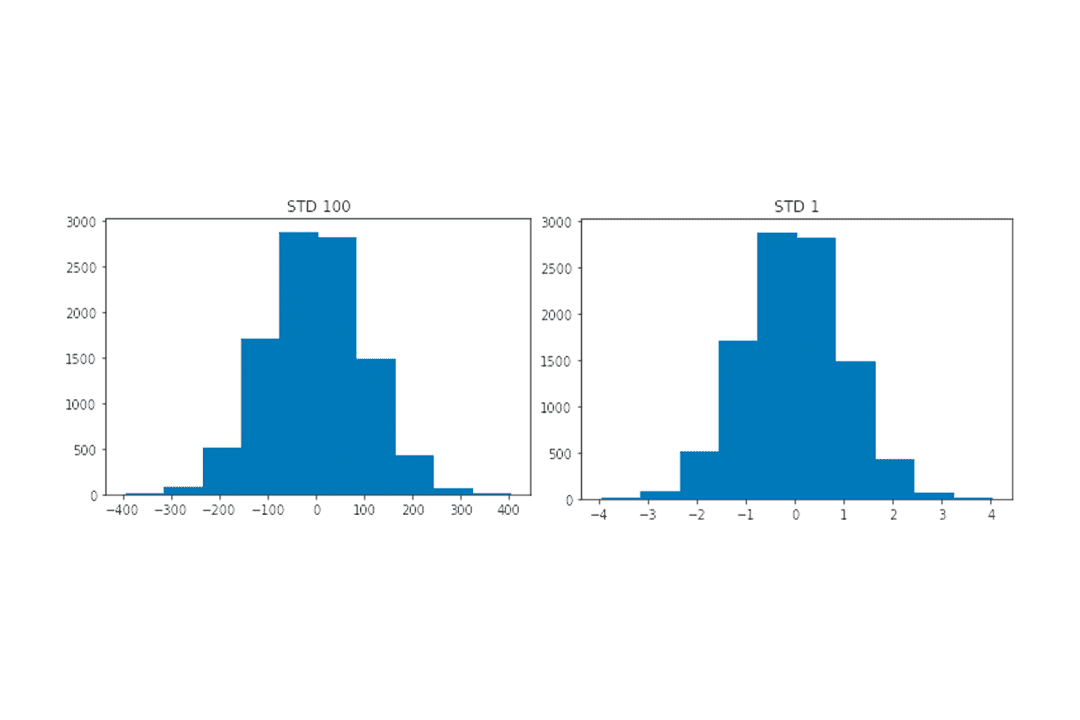
\includegraphics[width=\textwidth]{images/un-softmax-sol-diagram.png}
    \caption{STD Difference}
\end{figure}

In questo grafico si vedono 2 distribuzioni simili, ma che hanno una campana
una più piccola e una più larga. Questo dipenede dalla \textbf{Deviazione
    Standard}. Cosa entra in gioco in questo caso? $Softmax$. Se si fa il plot
della softmax, si vede che normalizzare permette di avere una scala.

\begin{figure}[H]
    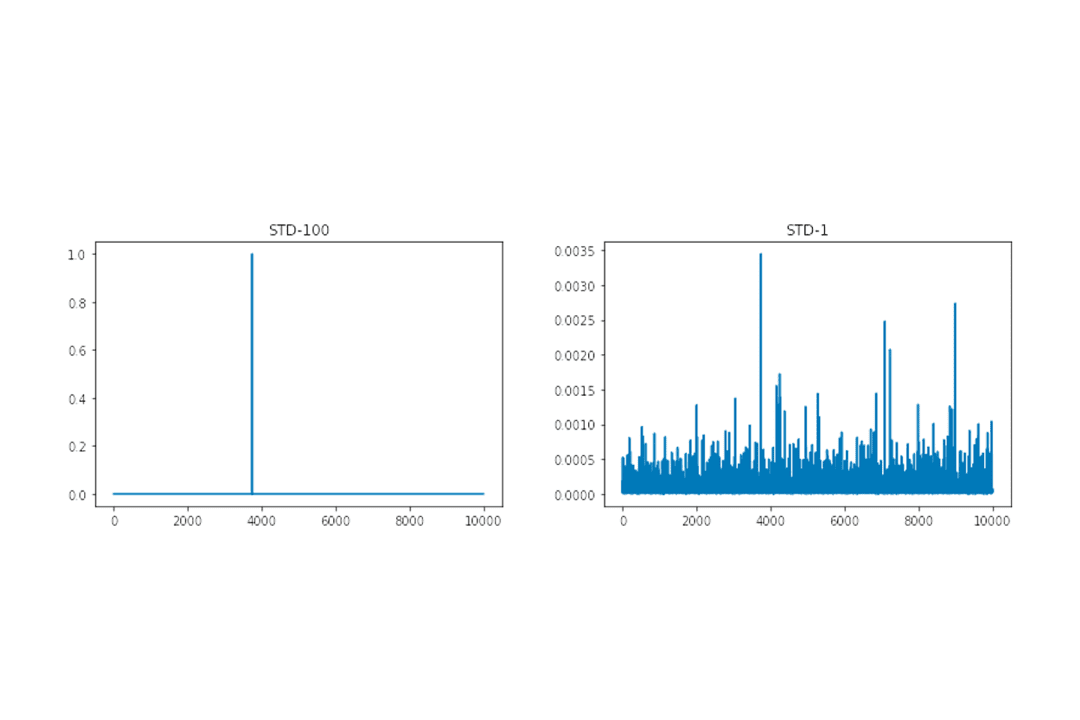
\includegraphics[width=\textwidth]{images/softmax-std-diagram.png}
    \caption{Softmax Plot}
\end{figure}

Come vediamo, quello con deviazione standard 1 fornisce una distribuzione che
permette al gradiente di propagarsi, non avendo il problema del
\textbf{vanishing gradient.}

La prossima versione sfrutta due matrici in input $Q$ e $X$ che hanno shape
$N_q, D_q$, e $N_x, D_q$. Questo porta ad avere una diversa output per il
softmax e come output finale.

\begin{figure}[H]
    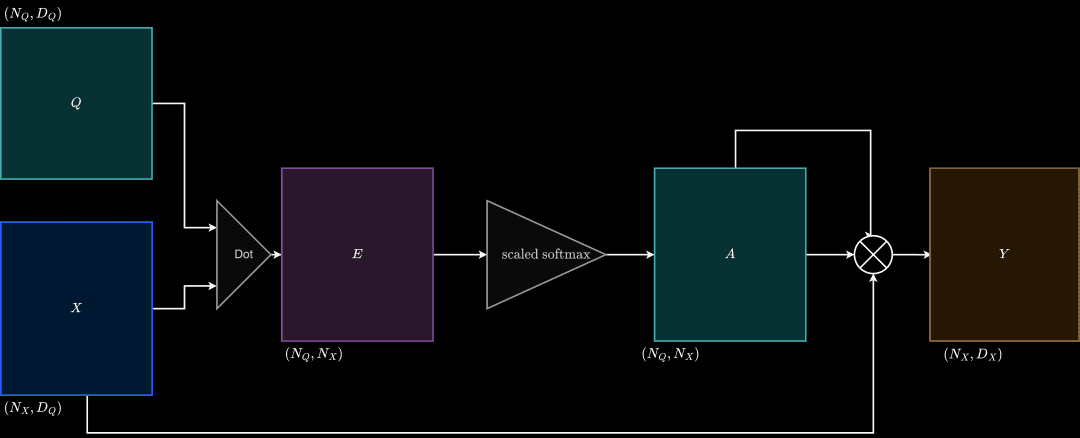
\includegraphics[width=\textwidth]{images/evolution-Version-3.png}
    \caption{Multihead Attention Versione 3}
\end{figure}

Nella $Versione \ 4$ si fanno dei cambiamenti nella versione di input. Si
divide l'input in coppie di matrici, rispettivamente \textbf{keys} e
\textbf{values}.
\begin{figure}[H]
    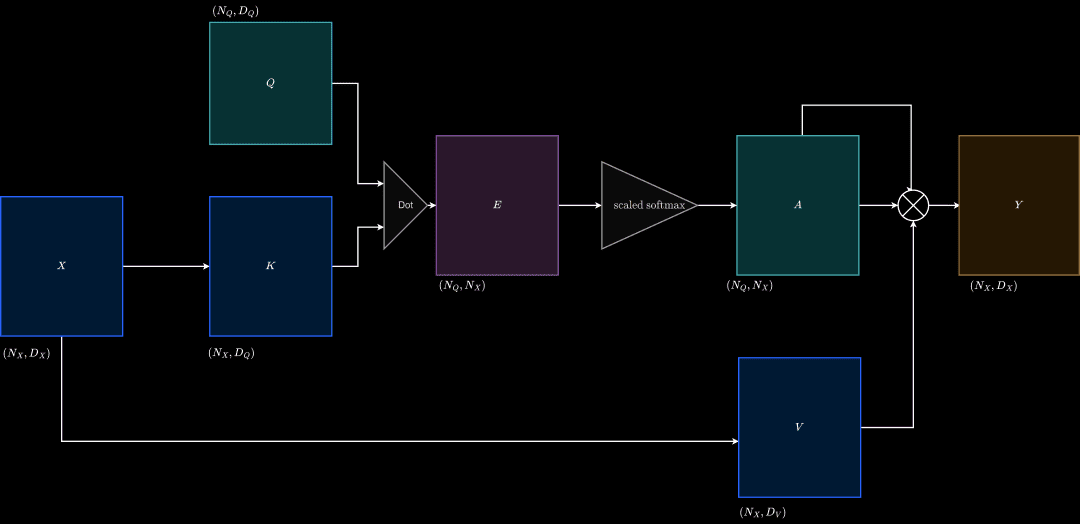
\includegraphics[width=\textwidth]{images/evolution-Version-4.png}
    \caption{Multihead Attention Versione 4}
\end{figure}

Per creare attenzione incrociata, apportiamo alcune modifiche. Le modifiche
sono specifiche della matrice di input. Come già sappiamo, l'attenzione
necessita di una matrice di input e di una matrice di query. Supponiamo di
proiettare la matrice di input in una coppia di matrici, vale a dire la matrice
chiave e quella valore .

La matrice chiave è curata rispetto alla matrice di query. Ciò si traduce in
pesi di attenzione. Qui la matrice dei valori viene trasformata con i pesi
dell'attenzione in contrapposizione alla trasformazione della matrice di input,
come visto in precedenza.

\begin{equation}
    \begin{aligned}
        K = X \cdot W_K \\
        V = X \cdot W_V \\
    \end{aligned}
\end{equation}

Questo viene fatto per disaccoppiare la complessità. La matrice di input può
ora avere una proiezione migliore che si occupa di costruire pesi di attenzione
e anche matrici di output migliori. La visualizzazione dell'attenzione
incrociata è mostrata nella Figura.

Nella $Versione \ 5$ fa riferimento alla $4$. Come abbiamo visto, ci sono 3
matrici: \textbf{Query, Keys, Values}. Sappiamo che le matrici keys e values
sono proiezioni delle matrici in input. E se facesimo come proiezione
dell'input anche la matrice di query?

\begin{equation}
    \begin{aligned}
        K = X \cdot W_K \\
        V = X \cdot W_V \\
        Q = X \cdot W_Q \\
    \end{aligned}
\end{equation}

\begin{figure}[H]
    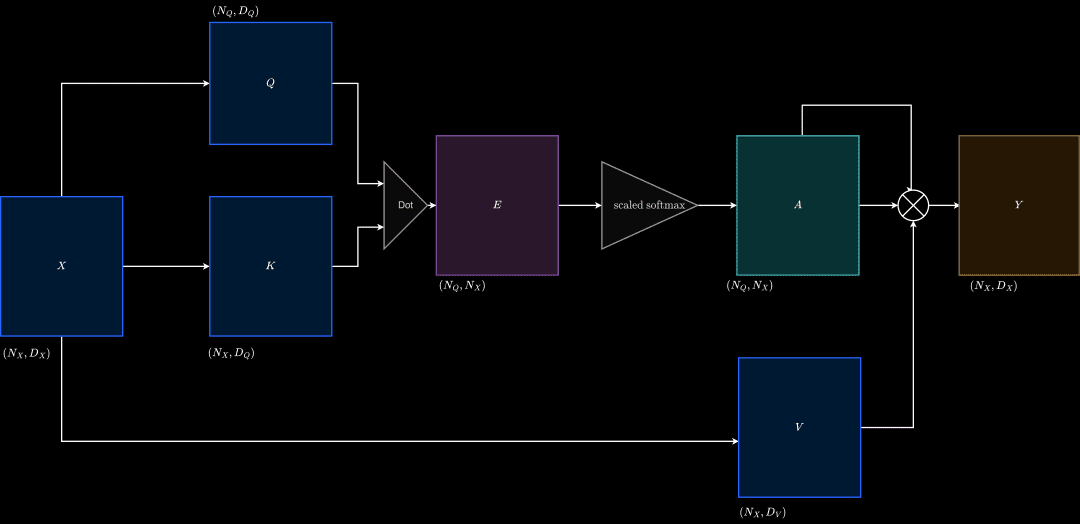
\includegraphics[width=\textwidth]{images/evolution-Version-5.png}
    \caption{Multihead Attention Versione 5}
\end{figure}

Nell'ultima versione, cioè la $Versione \ 6$, si parla di \textbf{multi-head
    attention}.

Le matrici di prima vengono proiettate ad un numero di teste. Gli splits
vengono passati ad un modulo di self attention, come abbiamo visto prima. Ogni
split viene poi \textbf{concatenato} in una singola rappresentazione.

\begin{figure}[H]
    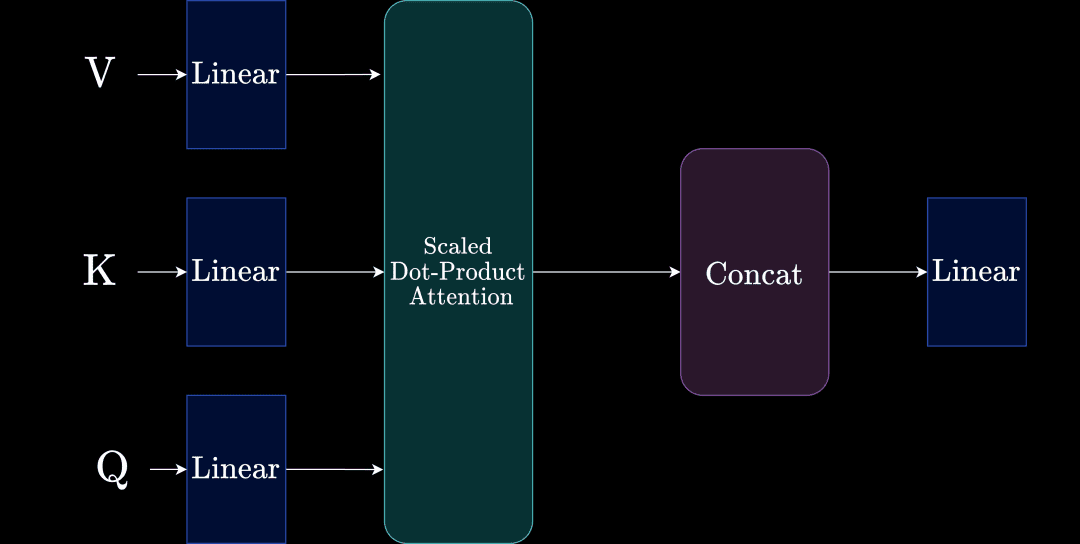
\includegraphics[width=\textwidth]{images/mha.png}
    \caption{Multihead Attention Versione 6}
\end{figure}

\subsection{Positional Encoding}

Se ci pensiamo, lavorando con matrici \textbf{non abbiamo il concetto di
    posizione} e di ordinamento. Per questo motivo, nell'architettura transformer
bisogna aggiungere l'informazione della posizione delle parole.

\begin{figure}[H]
    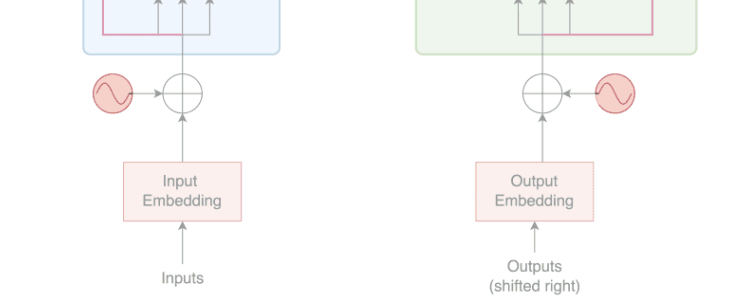
\includegraphics[width=\textwidth]{images/penc.png}
    \caption{Positional Encoding}
\end{figure}

Questi due nodi si occupano di aggiungere la posizione alla matrice di input.
In che modo, però? Per introdurlo, si sono usate 2 formule matematiche:

\begin{equation}
    \begin{aligned}
        PE_{pos, 2i} = sin \left( \frac{pos}{10000^{\frac{2i}{d_{model}}}} \right)   \\
        PE_{pos, 2i+1} = cos \left( \frac{pos}{10000^{\frac{2i}{d_{model}}}} \right) \\
    \end{aligned}
\end{equation}

Queste due sono le funzioni che vengono usate per aggiungere la posizione alla
matrice di input. \textbf{Ogni posizione} viene encodato in un
\textbf{vettore}.

\subsection{Come si allenano i transformers?}
Il concetto che si utilizza ormai è questo:

Transformer come BERT. Ecco una spiegazione più dettagliata di ciascuno dei
passaggi:

\begin{itemize}
    \item Si prende un dataset: Questo è il primo passo per l'allenamento di qualsiasi
          modello di machine learning. Il dataset dovrebbe consistere in una serie di
          esempi di testo. Per un modello di linguaggio, questo potrebbe essere un grande
          corpus di testo, come Wikipedia o un insieme di libri.
    \item Si creano delle coppie di testi (input con parole mascherate/nascoste, input):
          Questo passaggio descrive la creazione di esempi di allenamento per il modello.
          Per un modello come BERT, gli esempi di allenamento sono creati prendendo pezzi
          di testo dal dataset e mascherando alcune delle parole. Queste parole
          mascherate sono poi quelle che il modello cercherà di predire durante
          l'allenamento. Le coppie di testi quindi consistono nel testo con le parole
          mascherate (che funge da input per il modello) e il testo originale (che funge
          da "etichetta" o "obiettivo" per l'allenamento).
    \item Si fa l'allenamento per predire le parole mascherate/nascoste: Infine, il
          modello viene allenato per predire le parole mascherate basandosi sul contesto
          fornito dalle altre parole nell'input. L'obiettivo è che, dopo un sufficiente
          allenamento, il modello sarà in grado di utilizzare il contesto per "riempire
          gli spazi vuoti" in un pezzo di testo, il che è una competenza chiave per molte
          attività di elaborazione del linguaggio naturale.
\end{itemize}


Questi modelli \textbf{non sono fine-tunabili}. L'idea tipica non è fine tuning, ma \textbf{in context learning}.

\subsection{In Context Learning}

Immaginiamo di creare un app che ha un chatbot per un hotel. Le persone devono poterci interagire, richiedere camere, ecc\dots

\textbf{Scratch:} Fornire al sistema tutte le cose dellhotel. Costruire un transformer in base a questo.

\textbf{Usa un modello (Bert, GPT)}: Fornire il documento sul quale vuoi fare il fine tuning come prima frase di input del modello. Ad esempio, il documento di tutte le informazioni dell'hotel.

Ad esempio, scrivere per bene i passaggi nella richiesta del prompt fornisce risultati migliori e più precisi. 

Praticamente, non si programma niente e si inserisce solamente il contesto per salvarlo come stato del modello mentre lo si utilizza.
Si parla di \textbf{prompting engineering}.

\subsection{Few Shots learning}

Praticamente, in context learning ma oltre alla descrizione si forniscono degli \textbf{esempi} di quello che si vuole fare.
Questo per fare in modo per vedere se il modello riesce a generalizzare il problema e a risolvere il problema.
\newpage
\section*{Capitoli di laboratorio}
\section{Lab: Introduzione Python}
\subsection{MatPlotLib}

\subsubsection{Plots}

\begin{lstlisting}[language=Python]
import matplotlib.pyplot as plt
import numpy as np

x = np.linspace(0, 10, 100)
plt.plot(x, np.sin(x))
plt.show()
\end{lstlisting}

Non c'è molto da dire, il codice è autoesplicativo. La funzione \texttt{plot}
prende in input due array, uno per l'asse delle ascisse e uno per l'asse delle
ordinate. In questo caso, \texttt{x} è un array di 100 punti equidistanti tra 0
e 10, mentre \texttt{np.sin(x)} è un array di 100 punti che rappresentano il
seno dei punti di \texttt{x}. La funzione \texttt{show} mostra il grafico.

%fai la figure che è descritta nel codice

\begin{tikzpicture}
    \begin{axis}[
            axis lines = left,
            xlabel = $x$,
            ylabel = {$f(x)$},
        ]
        %Below the red parabola is defined
        \addplot [
            domain=0:10,
            samples=100,
            color=red,
        ]
        {sin(deg(x))};
        \addlegendentry{$\sin(x)$}
    \end{axis}
\end{tikzpicture}

\subsubsection{Sub-plots}

\begin{lstlisting}[language=Python]
import matplotlib.pyplot as plt
import numpy as np

x = np.linspace(0, 10, 100)
plt.subplot(2, 1, 1)
plt.plot(x, np.sin(x))
plt.subplot(2, 1, 2)
plt.plot(x, np.cos(x))
plt.show()

\end{lstlisting}

La funzione \texttt{subplot} prende in input tre parametri: il numero di righe,
il numero di colonne e l'indice del subplot corrente. Nel caso di questo
esempio, il subplot corrente è il primo, quindi viene mostrato il grafico del
seno. Poi viene mostrato il secondo subplot, che è quello del coseno.

\begin{tikzpicture}
    \begin{axis}[
            axis lines = left,
            xlabel = $x$,
            ylabel = {$f(x)$},
        ]
        %Below the red parabola is defined
        \addplot [
            domain=0:10,
            samples=100,
            color=red,
        ]
        {sin(deg(x))};
        \addlegendentry{$\sin(x)$}
    \end{axis}
\end{tikzpicture}

\begin{tikzpicture}
    \begin{axis}[
            axis lines = left,
            xlabel = $x$,
            ylabel = {$f(x)$},
        ]
        %Below the red parabola is defined
        \addplot [
            domain=0:10,
            samples=100,
            color=red,
        ]
        {cos(deg(x))};
        \addlegendentry{$\cos(x)$}
    \end{axis}
\end{tikzpicture}

C'è anche qui poco da dire, il codice è autoesplicativo.

\subsection{NumPy}

La libreria NumPy è una libreria per Python che permette di lavorare con
array multidimensionali. Per importare la libreria, basta scrivere
\texttt{import numpy as np}.

Mi rompo le palle in maniera assurda di scrivere tutti gli esempi. Quindi questo capitolo 
penso sia abbastanza inutile.


E' possibile trovare il codice di \textbf{numPy} a questo link: \url{www.ciao.it}
\newpage
\section{Lab: Reti Neurali da zero}
\subsection{Introduzione}

Partiamo dicendo una cosa molto importante: \textbf{per quale motivo usiamo la
    backpropagation?}
\begin{equation}
    \frac{y-b}{x} = w
\end{equation}

Ma possiamo scriverlo come:
\begin{equation}
    (y-b) \cdot x^{-1} = w
\end{equation}

Ora però, se consideriamo:
\begin{itemize}
    \item y il vettore risultante
    \item w la matrice dei pesi
    \item x il vettore di input
\end{itemize}

Calcolare l'inversa di \textbf{x} non è una cosa cosi poco costosa, anzi. Per
questo motivo utilizziamo il training delle reti come la backpropagation e la
discesa del gradiente.

Ora, andiamo più a fondo. Facciamo un esempio più pratico.

\subsection{Esempio pratico}

Immaginiamo di avere un dataset di 2 features e una label da identificate.
%make  atable with x_1 e x_2 and y, with 10 rows
\begin{table}[h!]
    \centering
    \begin{tabular}{|c|c|c|}
        \hline
        $x_1$ & $x_2$ & y \\
        \hline
        1     & 2     & 0 \\
        2     & 3     & 0 \\
        3     & 4     & 0 \\
        4     & 5     & 0 \\
        5     & 6     & 0 \\
        6     & 7     & 1 \\
        7     & 8     & 1 \\
        8     & 9     & 1 \\
        9     & 10    & 1 \\
        10    & 11    & 1 \\
        \hline
    \end{tabular}
    \caption{Dataset di esempio}
    \label{tab:my_label}
\end{table}

Ogni livello di una rete neurale può essere rappresentato attraverso le
\textbf{matrici}.

%fai un grafico di una rete neurale con 2 input, 1 hidden layer da 3 nodi e un output layer da 1 nodo
\begin{figure}[h!]
    \centering
    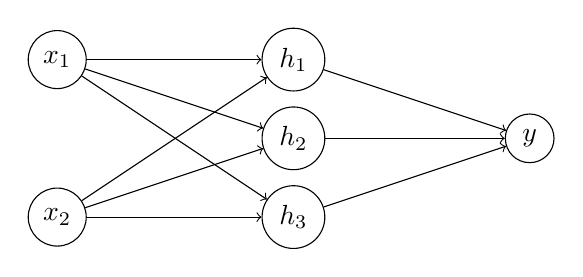
\begin{tikzpicture}
        \node[draw,circle] (x1) at (0,0) {$x_1$};
        \node[draw,circle] (x2) at (0,-2) {$x_2$};
        \node[draw,circle] (h1) at (3,0) {$h_1$};
        \node[draw,circle] (h2) at (3,-1) {$h_2$};
        \node[draw,circle] (h3) at (3,-2) {$h_3$};
        \node[draw,circle] (y) at (6,-1) {$y$};
        \draw[->] (x1) -- (h1);
        \draw[->] (x1) -- (h2);
        \draw[->] (x1) -- (h3);
        \draw[->] (x2) -- (h1);
        \draw[->] (x2) -- (h2);
        \draw[->] (x2) -- (h3);
        \draw[->] (h1) -- (y);
        \draw[->] (h2) -- (y);
        \draw[->] (h3) -- (y);
    \end{tikzpicture}
    \caption{Rete neurale di esempio}
    \label{fig:my_label}
\end{figure}

Ma passiamo alla definizione formale:

\textbf{Definizione Rete Neurale}: Una rete neurale è una tupla:
\begin{equation}
    NN = \{g,l,o,i,fpp\}
\end{equation}
con:
\begin{itemize}
    \item g: il grafico
    \item l: la funzione loss
    \item o: l'ottimizzatore
    \item i: l'inizializzatore
    \item fpp: la fix point procedure
\end{itemize}

\textbf{Nota 1:} l'ottimizzatore intende in quale modo si performa la \textbf{discesa del gradiente.}

\textbf{Nota 2:} l'inizializzatore è la funzione che inizializza i pesi della rete neurale. Ci possono essere diversi algoritmi per gli
inizializzatori, ma non c'è modo di sapere quale funziona meglio, poiché non si può sapere nelle reti neurali.

\subsubsection{Il grafo}

Il solito grafo che abbiamo visto in precedenza è un grafo aciclico diretto. Ha
dei nodi che sono i percettroni, che hanno degli archi composti dai pesi, che
hanno una funzione di attivazione, che prendono in input un valore e ne sputano
fuori uno chiamando la funzione di attivazione sull'input.

\textbf{Nota:} la funzione di attivazione è una funzione non lineare.

\subsubsection{La funnzione loss}

L'obiettivo della funzione loss è quello di misurare la distanza tra il valore
predetto e il valore reale.
\begin{equation}
    L(y,\hat{y}) = \frac{1}{2}(y-\hat{y})^2
\end{equation}

\subsubsection{L'ottimizzatore}

L'ottimizzatore ci permette di trovare una soluzione ottimale \textbf{non
    ottima}, cioé trovare \textbf{il minimo della funzione di loss}. La tecnica che
si usa è quella delle \textbf{discesa del gradiente}.

\subsubsection{Discesa del gradiente}

La discesa del gradiente sfrutta un parametro chiamato \textbf{learning rate}
che permette di capire quanto la discesa del gradiente deve essere veloce. Se
il learning rate è troppo alto, la discesa del gradiente potrebbe non
convergere, se è troppo basso, la discesa del gradiente potrebbe convergere
troppo lentamente.

\textbf{Nota:} il learning rate è un ottimizzatore \textit{molto naive}.

\subsubsection{Inizializzatore}

Il metodo di inizializzazione può cambiare di molto il risultato della rete
neurale. In pratica assegna un valore ai \textit{pesi} e ai \textit{bias}.
Alcuni metodi sono:
\begin{itemize}
    \item Inizializzazione a 0: Questo ha alcuni problemi, perché non si ha
          diversificazione tra i nodi e i nodi nascosti diventano simmetrici.
    \item inizializzazione costante: stessi problemi della precedente
    \item Inizializzazione Random: Si fa seguendo una distribuzione uniforme oppure una
          distribuzione normale.
\end{itemize}

\subsubsection{Fix Point Procedure}

La procedura per il training di una rete neurale è un processo che si basa su
alcuni steps:
\begin{lstlisting}

net CustomNeuralNetwork(...)
initialize_weights_and_biases (net)
optimizer = myOptimizer(...) 
loss_function = myLoss Function(...)
epochs = ... # the number of dataset scans
history = [] # a list containing the loss evolution
for epoch in range(epochs):
    optimizer.reset() # it may have an internal status
    loss = loss_fuction (out_target, net(input)) back_propagation (loss, optimizer, net)
    history.append(loss)
\end{lstlisting}

\subsection{Esempio da zero}
\subsubsection{La funzione Sigmoid}

Spendiamo qualche parola sulla funzione sigmoid, che è una funzione molto
importante per le reti neurali.

In particolare, la funzione avrà un valore di attivazione compreso tra 0 e 1 e,
in particolare, quando l'input è 0, la funzione ha valore 0.5. Se ha un valore
basso, sarà zero e chiaramente se sarà alto avrà valore 1.
\begin{figure}[H]
    \begin{center}
        \begin{tikzpicture}
            \begin{axis}[
                    axis lines = left,
                    xlabel = $x$,
                    ylabel = {$f(x)$},
                ]
                %Below the red parabola is defined
                \addplot [
                    domain=-10:10,
                    samples=100,
                    color=red,
                ]
                {1/(1+exp(-x))};
                \addlegendentry{$\frac{1}{1+e^{-x}}$}
            \end{axis}
        \end{tikzpicture}
    \end{center}
    \caption{Funzione Sigmoid}
\end{figure}

Detto questo, \textbf{per quale motivo è importante?} Se pensiamo
all'\textit{inizializzazione}, che tipi di valori è meglio avere? Avere tutti i
valori a zero porterebbe a valori simmetrici e quindi a problemi di
convergenza. Vogliamo dei valori di pesi che siano \textbf{distribuiti
    uniformemente intorno allo 0.}

\subsection{Tangente Iperbolica TanH}

La funzione TanH è una funzione che ha un valore di attivazione compreso tra -1
e 1 e, in particolare, quando l'input è 0, la funzione ha valore 0. Se ha un
valore basso, sarà -1 e chiaramente se sarà alto avrà valore 1.

\begin{figure}[H]
    \begin{center}
        \begin{tikzpicture}
            \begin{axis}[
                    axis lines = left,
                    xlabel = $x$,
                    ylabel = {$f(x)$},
                ]
                %Below the red parabola is defined
                \addplot [
                    domain=-10:10,
                    samples=100,
                    color=red,
                ]
                {tanh(x)};
                \addlegendentry{$tanh(x)$}
            \end{axis}
        \end{tikzpicture}
    \end{center}
    \caption{Funzione TanH}
\end{figure}

\subsection{ReLu}

La funzione ReLu è una funzione che ha un valore di attivazione pari a 0 quando
l'input è negativo e ha un valore di attivazione pari all'input quando l'input
è positivo.

\textbf{Parole di Adornetto:} E' buona? Si. E' stabile? Si. Perché? Boh.

\begin{figure}[H]
    \begin{center}
        \begin{tikzpicture}
            \begin{axis}[
                    axis lines = left,
                    xlabel = $x$,
                    ylabel = {$f(x)$},
                ]
                %Below the red parabola is defined
                \addplot [
                    domain=-10:10,
                    samples=100,
                    color=red,
                ]
                {max(0,x)};
                \addlegendentry{$max(0,x)$}
            \end{axis}
        \end{tikzpicture}
    \end{center}
    \caption{Funzione ReLu}
\end{figure}

\subsection{Scalare i valori}

Skip molto avanti riguardo l'esempio, ma si parla di scalare i dati.

Lo scaling dei dati è un'operazione importante nel machine learning perché i
dati possono essere su scale diverse e questo può causare problemi durante
l'allenamento del modello. Ad esempio, se abbiamo due variabili di input, una
che varia da 0 a 1 e l'altra che varia da 0 a 1000, la seconda variabile avrà
un impatto molto maggiore sull'output del modello rispetto alla prima. Ciò può
portare a problemi come l'overfitting, in cui il modello si adatta troppo ai
dati di addestramento e non generalizza bene sui dati di test.

Per risolvere questo problema, si utilizzano tecniche di scaling dei dati per
portare tutte le variabili su una scala comune. Ci sono diverse tecniche di
scaling, come la normalizzazione e la standardizzazione, che possono essere
utilizzate a seconda del tipo di dati e del modello utilizzato.

Le funzioni di attivazione, come la funzione ReLU, possono anche essere
influenzate dalla scala dei dati di input. Se i dati non sono scalati
correttamente, la funzione di attivazione potrebbe produrre valori che non
permettono un allenamento corretto del modello. Lo scopo dello scaling dei dati
è quello di mantenere i dati intorno allo 0, in modo che le funzioni di
attivazione possano produrre valori che permettono un allenamento corretto del
modello.

\begin{itemize}
    \item Standardizzazione: La standardizzazione è una tecnica di scaling dei dati che
          assume che i dati siano distribuiti normalmente all'interno di ogni feature e
          li scala in modo che la distribuzione abbia una media uguale a 0 e una
          deviazione standard uguale a 1. Questa tecnica funziona bene quando i dati
          hanno una distribuzione normale, ma non funziona bene se i dati hanno una
          distribuzione non normale.
    \item Normalizzazione: La normalizzazione è una tecnica di scaling dei dati che scala
          i valori di ogni feature in modo che siano compresi tra 0 e 1. Questa tecnica
          funziona bene quando i valori di input non hanno una distribuzione normale. Ad
          esempio, se i valori di input sono compresi tra 0 e 1000, la normalizzazione li
          porterà su una scala compresa tra 0 e 1.
\end{itemize}

\subsection{Plottare la loss}

La funzione loss è una misura dell'errore del modello durante
l'allenamento. L'obiettivo dell'allenamento è quello di minimizzare la funzione
loss, ovvero di ridurre l'errore del modello. Durante l'allenamento, il modello
viene eseguito su un set di dati di addestramento e la funzione loss viene
calcolata per ogni esempio di addestramento. L'errore totale del modello è la
somma di tutte le funzioni loss per ogni esempio di addestramento.

L'allenamento del modello avviene in epoche, ovvero in cicli di esecuzione su
tutti i dati di addestramento. L'obiettivo è che la funzione loss diminuisca ad
ogni epoca, ovvero che l'errore del modello diminuisca man mano che il modello
viene addestrato su più dati. Se la funzione loss non diminuisce ad ogni epoca,
significa che il modello non sta imparando abbastanza dai dati di addestramento
e potrebbe essere necessario modificare l'architettura del modello o i
parametri di addestramento.

Se la funzione di loss arriva a 0, vuol dire che \textbf{siamo in minimo globale}, che non è comune.

%make a plot with x = epochs and y = loss and loss reaches 0 at the end, with a curve that goes down
\begin{figure}[H]
    \begin{center}
        \begin{tikzpicture}
            \begin{axis}[
                    axis lines = left,
                    xlabel = $epochs$,
                    ylabel = {$loss$},
                ]
                %Below the red parabola is defined
                \addplot [
                    domain=0:10,
                    samples=100,
                    color=red,
                ]
                {1/(1+exp(x))};
                \addlegendentry{$loss$}
            \end{axis}
        \end{tikzpicture}
    \end{center}
    \caption{Funzione loss}
\end{figure}


Se invece finiami con un grafico che arriva fino a 0.1 e poi si stabilizza, 
potremmo essere in un \textbf{minimo locale}, oppure semplicemente la topologia della Rete
permette di avere questo risultato come massimo risultato.


\subsection{Importante cosa su Gradient Descent}

Lo usiamo per un motivo particolare:
\begin{quote}
    Più andiamo indietro nei layer della rete, maggiori saranno i termini 
    che abbiamo già calcolato, rendendo i calcoli più efficienti.
\end{quote}
Questo è più semplice rispetto ad invertire una matrice
\newpage
\section{TensorFlow e Keras}

Onestamente non so cosa scrivere in questo capitolo. Se trovo qualcosa di
interessante la scrivo.

La lezione è fatta su un notebook. Quindi scriverò le notebook

\subsection{One Hot Encoding}

Sulle categoriche lo si fa quando si ha \textbf{una classificazione di classe}.
Ad esempio, se abbiamo una categorica che viene rappresentata numericamente,
\textbf{overall condition of the house}, se ha una scala da 1 a 10, in questo
caso \textbf{NON SERVE} il one hot encoding.

Se invece fosse stato qualcosa del tipo \textbf{House Color = 1,2,3}, in questo
caso si.

Diciamo che serve quando \textbf{NON ABBIAMO UNA SCALA NUMERICA o ORDINE}

\subsection{Variabili correlate}

Se abbiamo due variabili correlate, ad esempio \textbf{Overall Condition} e
\textbf{Overall Quality}, in questo caso \textbf{una delle due deve sparire.}
Le motivazioni sono due:
\begin{itemize}
    \item Ridurre la complessità del modello
    \item Evitare che la rete neurale NON RIESCA a dare il peso corretto alla variabile,
          poiché potrebbe dividere il peso in 50\% tra le due.
\end{itemize}

\subsection{Accuracy come loss}

Non usiamo l'accuracy come loss function perché dobbiamo usare una funzione che
sia \textbf{differenziabile}, e l'accuracy non lo è.

Nel nostro esempio usiamo \textbf{la binary cross entropy}.

\subsection{Epoche e batch size}

Capiamo questa cosa: ad ogni \textbf{epoca} dobbiamo scorrere l'intero dataset.
Ma ad ogni \textbf{iterazione di training NON CI SERVE l'intero dataset}.
Quindi, ad ogni epoca, dobbiamo scorrere il dataset \textbf{numero di
    iterazioni} volte.

Ad esempio, se abbiamo una batch size di 32, e abbiamo 1000 dati, allora
abbiamo 32 iterazioni per epoca.

\subsection{Overfitting e come evitarlo}

La definizione migliore di overfitting sentita: \textbf{dobbiamo imparare la
    distribuzione dei dati e non i dati stessi.}

Il nostro modello deve essere capace di \textbf{generalizzare}. In un grafico
dove abbiamo una validation loss, se la validation comincia a risalire dopo un
certo periodo di tempo non è capace di generalizzazione e vuol dire che non ha
imparato bene dai dati la loro distribuzione.

\subsection{Migliorare le performance di un modello}

Ci sono varie tecniche per migliorare le performance.

\begin{itemize}
    \item Aumentare il numero di epoche
    \item Aumentare il numero di neuroni
    \item Aumentare il numero di layer
    \item Cambiare la funzione di attivazione
\end{itemize}

\textbf{Attenzione:} Se si esagera con questi valori si può andare in overfitting.

Una tecnicha è quella della \textbf{regolarizzazione}. L'abbiamo vista anche in
\textbf{figura \ref{fig:regularization}}.%cita regolarizzazione in fig:regularization

\begin{lstlisting}[language=Python]
    model_3 = Sequential([
    Dense(1000, activation='relu', kernel_regularizer=regularizers.l2(0.01), input_shape=(10,)),
    Dropout(0.3),
    Dense(1000, activation='relu', kernel_regularizer=regularizers.l2(0.01)),
    Dropout(0.3),
    Dense(1000, activation='relu', kernel_regularizer=regularizers.l2(0.01)),
    Dropout(0.3),
    Dense(1000, activation='relu', kernel_regularizer=regularizers.l2(0.01)),
    Dropout(0.3),
    Dense(1, activation='sigmoid', kernel_regularizer=regularizers.l2(0.01)),
])
\end{lstlisting}

Nel notebook si vedono 3 grafici:
\begin{itemize}
    \item La rete normale: si comporta bene
    \item La rete più complessa: si comporta male perché overfitta 
    \item La rete più complessa regolarizzata: è la migliore
\end{itemize}
\section{Lab: Convolutional Neural Networks}

\subsection{Cross Entropy vs Accuracy}

\begin{domanda}(Per quale motivo usiamo la cross entropy nella multi-class classification? Perché non accuracy?)
\end{domanda}

Se prendessimo un esempio di classificazione con 3 classi $1,2,3$ e due
classificatori. Immaginiamo di avere degli examples che hanno \textbf{true
    class label}:

\begin{itemize}
    \item 0 0 1
    \item 0 1 0
    \item 1 0 0
\end{itemize}

E avessimo due classificatori che hanno come risultato:

%tablella con 3 righe e 3 colonne
\begin{table}[H]
    \centering
    \textbf{Classificatore 1:}

    \begin{tabular}{|c|c|c|}
        \hline
        \textbf{Example 1} & \textbf{Example 2} & \textbf{Example 3} \\
        \hline
        0.1                & 0.1                & 0.8                \\
        \hline
        0.1                & 0.8                & 0.1                \\
        \hline
        0.4                & 0.5                & 0.1                \\
        \hline
    \end{tabular}
\end{table}

\begin{table}[H]
    \centering
    \textbf{Classificatore 2:}

    \begin{tabular}{|c|c|c|}
        \hline
        \textbf{Example 1} & \textbf{Example 2} & \textbf{Example 3} \\
        \hline
        0.3                & 0.3                & 0.4                \\
        \hline
        0.3                & 0.4                & 0.3                \\
        \hline
        0.4                & 0.5                & 0.1                \\
        \hline
    \end{tabular}
\end{table}


Entrambi hanno un'\textbf{accuracy} del $0.66$ ma il \textbf{classificatore 1} è
più sicuro delle sue predizioni. La \textbf{cross entropy} è una funzione che
misura la \textbf{distanza} tra due distribuzioni di probabilità. In questo caso
misura la distanza tra la distribuzione di probabilità del classificatore e la
distribuzione di probabilità delle \textbf{true class label}. La cross entropy
è definita come:

\begin{equation}
    H(p,q) = - \sum_{x} p(x) \log q(x)
\end{equation}

Dove $p$ è la distribuzione di probabilità delle \textbf{true class label} e $q$
è la distribuzione di probabilità del classificatore. 


\subsection{Workflow per image classification}


\begin{lstlisting}[language=Python, caption=Workflow per image classification]
img_size=(50,50)

images = []
age = []
gender = []
for img in os.listdir(path):
  ages = img.split("_")[0]
  
  if int(ages) <18 or int(ages)>25:
    continue
  
  genders = img.split("_")[1]
  img = cv2.imread(str(path)+"/"+str(img))
  img = cv2.cvtColor(img,cv2.COLOR_BGR2RGB)
  img = cv2.resize(img, img_size, interpolation = cv2.INTER_AREA)
  images.append(np.array(img))
  age.append(np.array(ages))
  gender.append(np.array(genders))

\end{lstlisting}

In questo caso, vogliamo creare un modello per classificare \textbf{gender} e \textbf{age}. Facciamo un po' di modifiche alla dimensione
delle immagini e le salviamo ciò che ci serve in un array.

\begin{lstlisting}[language=Python, caption=Workflow per image classification]
age = np.array(age,dtype=np.int64)
images = np.array(images) / 255.  
gender = np.array(gender,np.uint64)

n=9
idx_toplot = np.random.randint(len(images), size=n)
plt.figure(figsize=(10, 10))
for i in range(n):
  ax = plt.subplot(3, 3, i + 1)
  plt.imshow(images[idx_toplot[i]])
  plt.title(f'Age={age[idx_toplot[i]]}, Gender={gender[idx_toplot[i]]}')
  plt.axis('off')
\end{lstlisting}

\subsubsection{Bilanciare le classi}

Se ci sono problemi di \textbf{unbalance} tra le classi di un dataset, ciò che si può fare per bilanciare 
le classi è \textbf{aumentare} il numero di esempi della classe con meno esempi. In questo caso,
possiamo fare \textbf{data augmentation} per aumentare il numero di esempi per ogni classe che 
ha meno esempi.

\begin{lstlisting}[language=Python, caption=Data augmentation]
data_augmentation = tf.keras.Sequential(
  [
    layers.RandomFlip("horizontal",input_shape=(img_size[0],img_size[1],3)),
    layers.RandomRotation(0.1),
    layers.RandomZoom(0.1),
  ]
)

# Find the class to be augmented and the major one
minor_class = min(gender_class_counts, key=gender_class_counts.get)
major_class = max(gender_class_counts, key=gender_class_counts.get)

# Select the images belonging to the class to augment
img_seeds = images[gender==minor_class]

# Select random indexes for the images to augment
n_augment = gender_class_counts[major_class]-gender_class_counts[minor_class]
idx_to_aug = np.random.randint(img_seeds.shape[0], size=n_augment)

new_images = []
new_gender = []
plt.figure(figsize=(10, 10))
for i in range(n_augment):
  augmented_image = data_augmentation(img_seeds[idx_to_aug[i]])
  new_images.append(augmented_image)
  new_gender.append(minor_class)

  if i<9:
    ax = plt.subplot(3, 3, i + 1)
    plt.imshow(augmented_image)
    plt.axis("off")
\end{lstlisting}

A questo punto, dopo aver \textbf{aumentato} il numero di esempi della classe minore, arriviamo ad avere 
un dataset bilanciato tra le due classi. Per quanto riguarda il modello, solita roba.

\begin{lstlisting}[language=Python, caption=Modello]
x_train_age, x_test_age, y_train_age, y_test_age = train_test_split(images, age, random_state=42)

x_train_gender, x_test_gender, y_train_gender, y_test_gender = train_test_split(balanced_images, balanced_gender, random_state=42)

gender_model = Sequential()

gender_model.add(Conv2D(32, kernel_size=3, activation='relu', input_shape=(img_size[0],img_size[1],3)))
gender_model.add(MaxPool2D(pool_size=3, strides=2))

gender_model.add(Conv2D(64, kernel_size=3, activation='relu'))
gender_model.add(MaxPool2D(pool_size=3, strides=2))

gender_model.add(Conv2D(128, kernel_size=3, activation='relu'))
gender_model.add(MaxPool2D(pool_size=3, strides=2))

gender_model.add(Flatten())
gender_model.add(Dropout(0.2))
gender_model.add(Dense(128, activation='relu'))
gender_model.add(Dense(1, activation='sigmoid', name='gender'))

gender_model.compile(optimizer='adam', loss='binary_crossentropy', metrics=['accuracy'])

history_gender = gender_model.fit(x_train_gender, y_train_gender,
                        validation_data=(x_test_gender, y_test_gender), epochs=10)

###########################
gender_model.save(save_model_path+'gender_model.h5')
###########################

\end{lstlisting}

\begin{domanda}(Per quale motivo utilizziamo la funzione \textbf{save}?)
\end{domanda}

Perché vogliamo salvare il modello che abbiamo creato in un file. In questo caso, il modello viene salvato
in un file \textbf{.h5}. Salviamo \textbf{i pesi della rete} per poter continuare in un secondo momento
l'addestramento della rete.

\begin{osservazione}(Cosa impara la rete?)
\end{osservazione}

La parte di convoluzione CNN impara a riconoscere le \textbf{features} delle immagini. La parte di
\textbf{Dense} impara a classificare le immagini in base alle features che ha imparato la parte di convoluzione.
\section{Autoencoders}

\subsection{Nota su PCA}

La PCA (Principal Component Analysis) è una tecnica di riduzione della
dimensionalità che si basa sulla decomposizione in autovalori della matrice di
covarianza.

Ora, immaginiamo di avere tre input $x_1, x_2, x_3$. Un \textbf{neurone} può
essere visto come una combinazione lineare di questi tre input, ovvero:

\begin{equation}
    y = w_1x_1 + w_2x_2 + w_3x_3
\end{equation}

\subsection{Autoencoders}

E' un architettura che permette di \textbf{proiettare} il nostro input in uno
\textbf{spazio dimensionale più piccolo}.

Avendo un input $x_1, x_2, x_3$, la rete ci darà come \textit{output} la
\textbf{ricostruzione} dell'input.

\begin{quote}
    Obiettivo: minimizzare la differenza tra l'input e la sua ricostruzione
\end{quote}

%Grafico di una rete con input x1,x2,x3. primo layer nascosto 3 nodi, secondo layer 2 nodi, terzo layer 3 nodi, output x1',x2',x3'

\begin{figure}[H]
    \begin{center}
        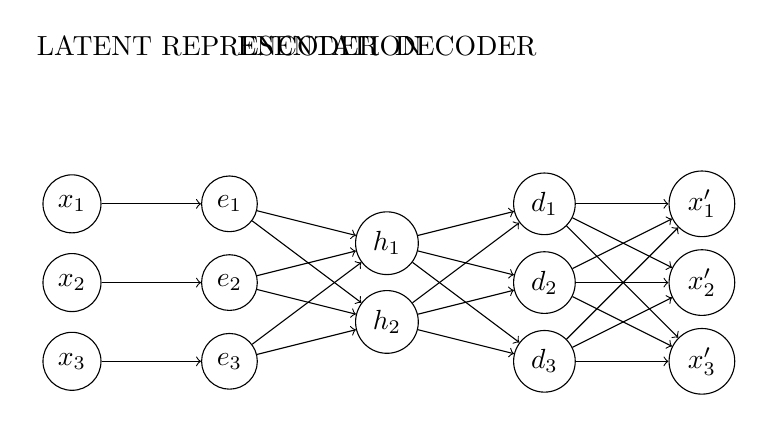
\begin{tikzpicture}
            \node[draw, circle] (x1) at (0, 0) {$x_1$};
            \node[draw, circle] (x2) at (0, -1) {$x_2$};
            \node[draw, circle] (x3) at (0, -2) {$x_3$};
            \node[draw, circle] (e1) at (2, 0) {$e_1$};
            \node[draw, circle] (e2) at (2, -1) {$e_2$};
            \node[draw, circle] (e3) at (2, -2) {$e_3$};

            %draw 2 nodes between the output and the hidden layer

            \node[draw, circle] (h1) at (4, -0.5) {$h_1$};
            \node[draw, circle] (h2) at (4, -1.5) {$h_2$};

            \node[draw, circle] (d1) at (6, 0) {$d_1$};
            \node[draw, circle] (d2) at (6, -1) {$d_2$};
            \node[draw, circle] (d3) at (6, -2) {$d_3$};

            \node[draw, circle] (xp1) at (8, 0) {$x'_1$};
            \node[draw, circle] (xp2) at (8, -1) {$x'_2$};
            \node[draw, circle] (xp3) at (8, -2) {$x'_3$};

            %write over D_1, D_2, D_3 the text ENCODER
            \node[draw=none] (t1) at (3, 2) {ENCODER};
            \node[draw=none] (t1) at (5, 2) {DECODER};
            \node[draw=none] (t1) at (2, 2) {LATENT REPRESENTATION};

            \draw[->] (x1) -- (e1);
            \draw[->] (x2) -- (e2);
            \draw[->] (x3) -- (e3);

            \draw[->] (e1) -- (h1);
            \draw[->] (e2) -- (h1);
            \draw[->] (e3) -- (h1);

            \draw[->] (e1) -- (h2);
            \draw[->] (e2) -- (h2);
            \draw[->] (e3) -- (h2);

            \draw[->] (h1) -- (d1);
            \draw[->] (h1) -- (d2);
            \draw[->] (h1) -- (d3);

            \draw[->] (h2) -- (d1);
            \draw[->] (h2) -- (d2);
            \draw[->] (h2) -- (d3);

            \draw[->] (d1) -- (xp1);
            \draw[->] (d2) -- (xp1);
            \draw[->] (d3) -- (xp1);

            \draw[->] (d1) -- (xp2);
            \draw[->] (d2) -- (xp2);
            \draw[->] (d3) -- (xp2);

            \draw[->] (d1) -- (xp3);
            \draw[->] (d2) -- (xp3);
            \draw[->] (d3) -- (xp3);

        \end{tikzpicture}
    \end{center}
\end{figure}
\begin{equation}
    Loss(\bar{x}, \bar{x'})
\end{equation}

L'\textbf{autoencoder} è praticamente l'unione tra \textbf{encoder, latent
    representation e decoder}.

\begin{domanda}(Per quale motivo usiamo le NN e non le PCA?)
\end{domanda}

La risposta è che le \textbf{PCA} sono lineari, e quindi meno complesse. Per
questo motivo, le NN sono più flessibili e possono essere usate per risolvere
problemi più complessi.

\subsubsection{Gli steps}

\begin{enumerate}
    \item Encoder: Impara una \textbf{rappresentazione compatta} dell'input
    \item Decoder: Ricostruisce l'input
\end{enumerate}

\subsubsection{Applicazioni}

Gli autoencoders possono essere usati in vari campi.

Ad esempio, forzare $x = r$. Questo porta ad un \textbf{rischio di overfitting
    elevato}. Diminuisce la dimensione e apprendimenti delle feature.

La vera potenza però è nell'\textbf{astrarre i dati} invece di impararli in
modo perfetto. Stiamo parlando di \textbf{produrre dati} che potrebbero
appartenere al dominio di input. Questo rientra in \textbf{data generation, data completion}.

Gli autoencoders non sono perfetti e soffrono di alcuni problemi. Alcuni sono:
\begin{itemize}
    \item Overfitting
    \item Grandezza del codice
\end{itemize}

Se vuoi copiarti le slides e aggiungere qualcosa.

\subsection{Autoencoders e Convolution}

Ricordiamo il concetto di fare sampling nello spazio latente. Questo è
fondamentale per la generazione di nuovi dati.

\begin{figure}[H]
    \begin{center}
        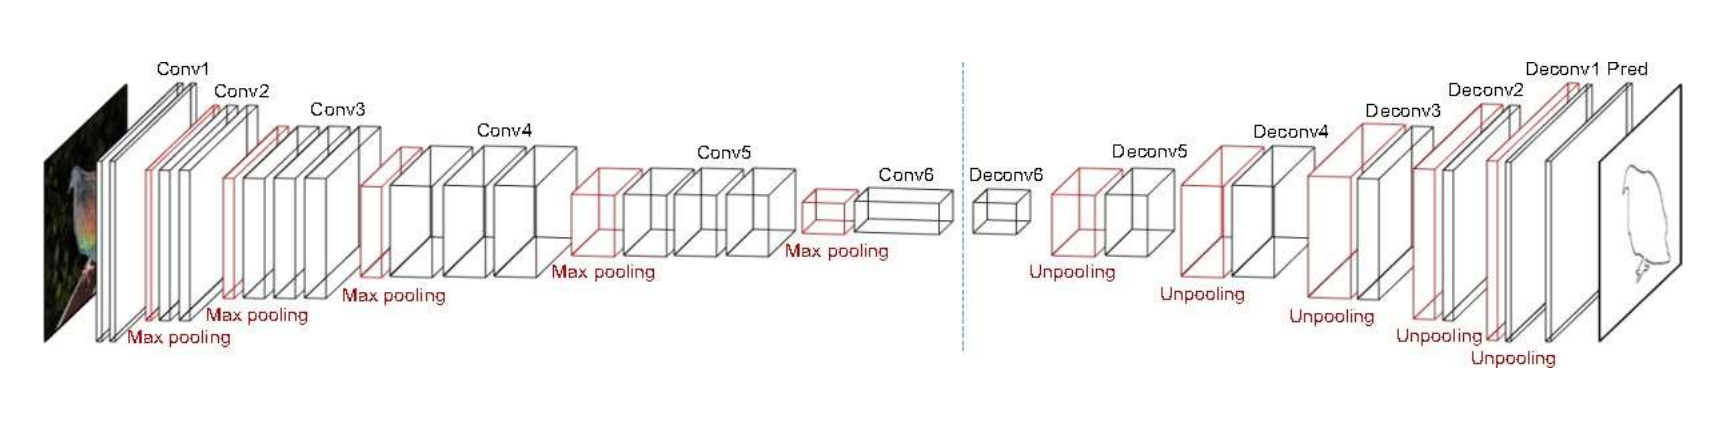
\includegraphics[scale=0.3]{images/autoencoders.png}
        \caption{Convolutional Autoencoder}
    \end{center}
\end{figure}

\begin{figure}[H]
    \begin{center}
        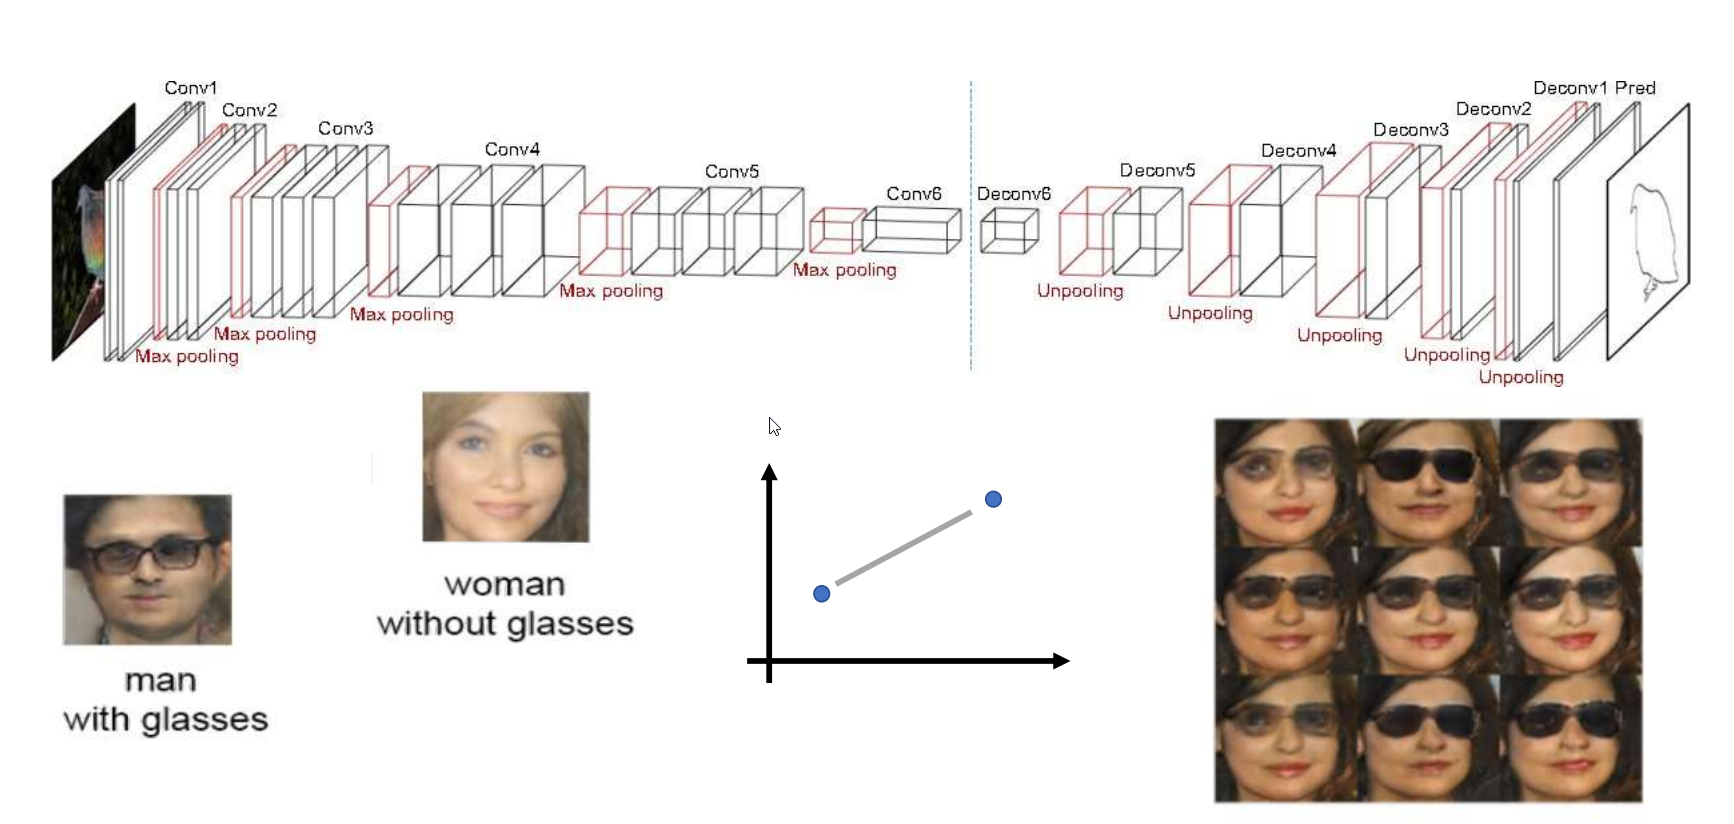
\includegraphics[scale=0.3]{images/autoencoders2.png}
        \caption{Convolutional Autoencoder sampling}
    \end{center}
\end{figure}

Praticamente, questa tecnologia è alla base per i \textbf{Deep Fakes!}

Altre informazioni: Notebook su autoencoders.
\newpage
\section{VAE (Variational Autoencoder)}

I VAE permettono di costruire un \textbf{latent space continuo}; Permette di
prendere uno spazio e un sample da quello spazio e saremo certi che i punti
all'interno seguono la distribuzione di quello spazio.

\textbf{Nota:} Se prendiamo un input, lo codifichiamo, quando sarà nel \textbf{latent space} non sarà più un punto,
ma sarà una distribuzione di punti. Non si codificano punti, quindi, ma \textbf{distribuzioni} (coppie di \textit{mean e standard deviation $\mu, \sigma$
}). La distribuzione sarà \textbf{normale}.

\begin{figure}[H]
    \centering
    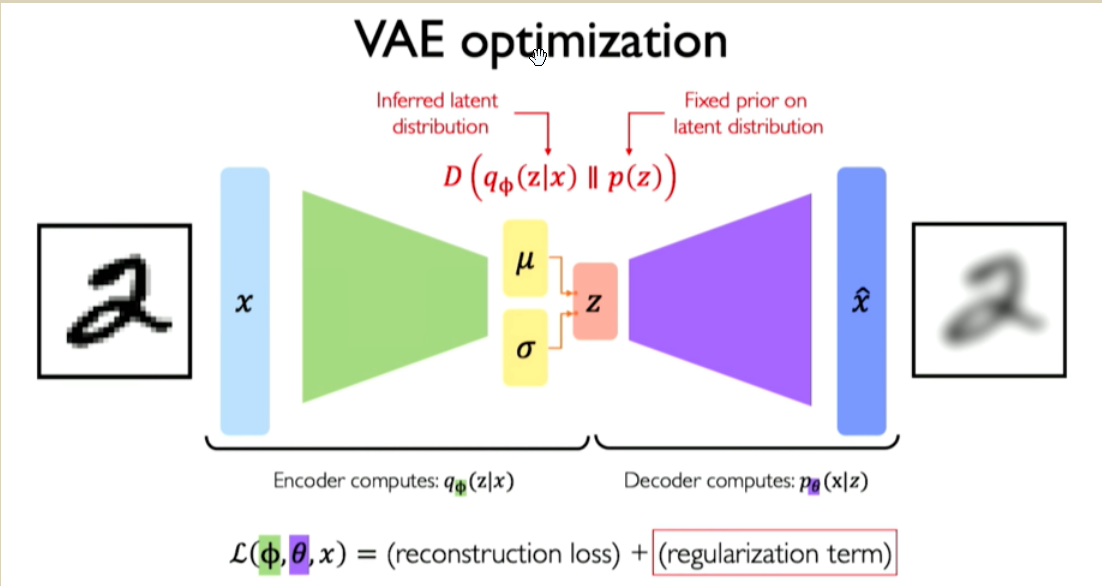
\includegraphics[width=0.7\textwidth]{images/vae.png}
\end{figure}

\begin{equation}
    D(q_\theta(z|x)||p(z))
\end{equation}

\textbf{Elementi:}
\begin{itemize}
    \item Inferred Latent Distribution: Distribuzione che hanno i dati di input
    \item Fixed Prior Latent Distribution: Distribuzione che vogliamo avere nel latent
          space
\end{itemize}

\textbf{Ad esempio}, nei normali Autoencoder, abbiamo che la distribuzione di input e la distribuzione di $z$ che viene fuori
non hanno niente a che fare. Cioè, non sappiamo niente a riguardo e non ci interessa.
Nei VAE, invece, vogliamo che la distribuzione di $z$ sia \textbf{normale}, perché con la distribuzione normale
si lavora in modo più stabile.

\begin{enumerate}
    \item Input X
    \item Decodifica X
    \item Si hanno due vettori di medie e varianze
    \item Si fa sampling e si ottiene $z$
    \item Si decodifica z
    \item Si ottiene il sample generato X'
\end{enumerate}

L'output di questa architettura prende il nome di \textbf{generated sample}.

Parlare di differenza tra regolarized e non regolarized dopo (inizio notebook)

\subsection{Regularization term e Reparametrization trick}

Il \textbf{Regularization Term} serve per fare in modo che la rete apprenda la
distribuzione nel \textbf{latent space}. Questo permtte di forzare di avere
$\mu = 0 \land \sigma = 1$

Il regularization term si chiama KL-Divergence e si calcola come segue:
\begin{equation}
    \frac{1}{2}\sum_{j=0}^{k-1}(\sigma_j+\mu^2_j - 1 - log(\sigma_j))
\end{equation}

\begin{figure}
    \centering
    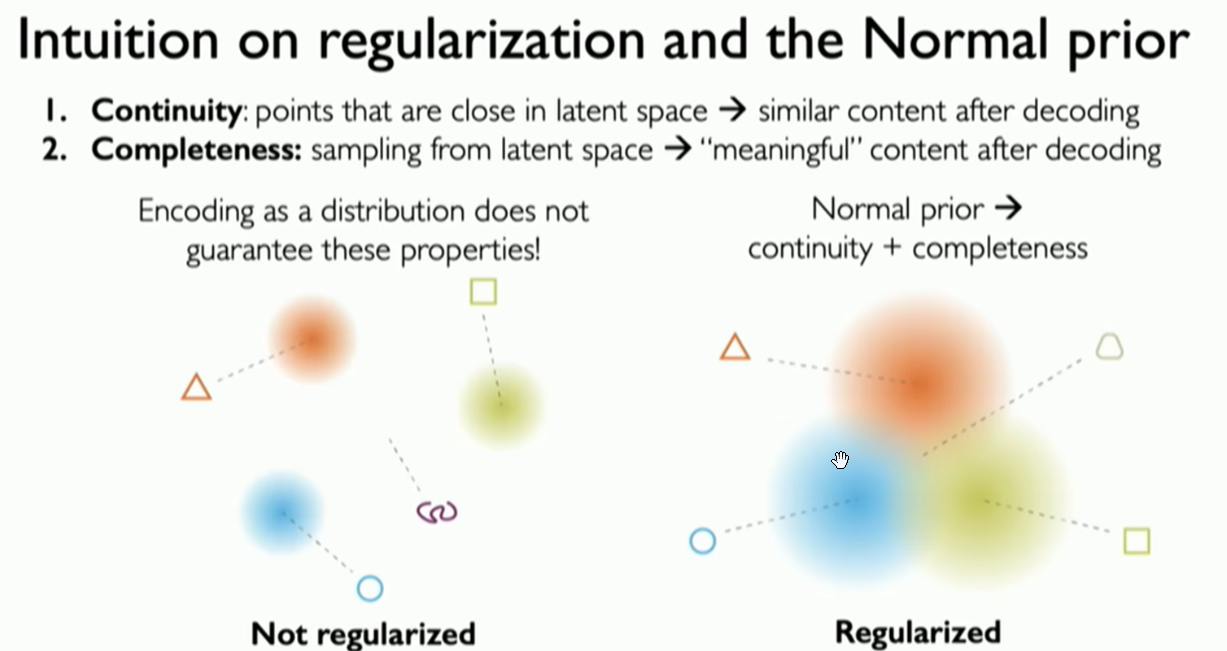
\includegraphics[width=0.7\textwidth]{images/vae2.png}
    \caption{Esempio di VAE}
\end{figure}

\begin{domanda}(Qual è la condizione per trainare una NN?)
\end{domanda}

Che la funzione sia \textbf{differenziabile}. Ma abbiamo un problema. Se dal
tra \textbf{mean e standard deviation} facciamo sampling, otteniamo una
distribuzione. Questo \textbf{non è differenziabile}. E qui entra in gioco il
\textbf{reparametrization trick}. Il trick è quello di \textbf{wrappare} questo
processo in una funzione che sia differenziabile.

\begin{figure}[H]
    \centering
    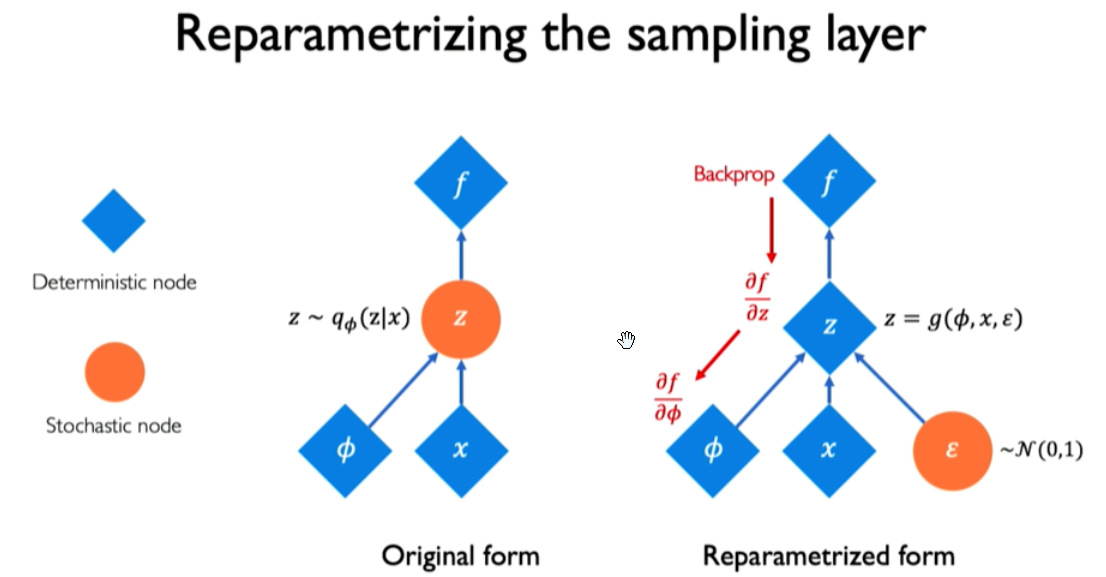
\includegraphics[width=0.7\textwidth]{images/reparametrization.png}
    \caption{Reparametrization trick}
\end{figure}

Oltre all'input, si aggiunge un elemento $\varepsilon$ che è un sample da una
distribuzione normale, lo consideriamo come \textbf{noise}. Questo noise è
\textbf{non deterministico} ed è differenziabile.

In questo modo, la funzione è differenziabile e si può fare backpropagation,
andando a cambiare i pesi dell'\textbf{encoder} e del \textbf{decoder}.

Senza di questo non potremmo farlo perché $z$ è un \textbf{random process} e
non è differenziabile.

\begin{lstlisting}[language=Python, caption={Esempio di VAE}]
from tensorflow import keras 

class Sampling(keras.layers.Layer):
    """Uses (z_mean, z_log_var) to sample z, the vector encoding a digit."""

    def call(self, inputs):
        z_mean, z_log_var = inputs
        batch = tf.shape(z_mean)[0]
        dim = tf.shape(z_mean)[1]
        epsilon = tf.keras.backend.random_normal(shape=(batch, dim))
        return z_mean + tf.exp(0.5 * z_log_var) * epsilon

from tensorflow.keras.datasets import fashion_mnist
import numpy as np

(x_train, _), (x_test, _) = fashion_mnist.load_data()
mnist_fashion = np.concatenate([x_train, x_test], axis=0)
mnist_fashion = np.expand_dims(mnist_fashion, -1).astype("float32") / 255

mnist_fashion.shape
\end{lstlisting}

\begin{lstlisting}[language=Python, caption={Esempio di VAE}]
    
latent_dim = 50
#50 medie e 50 deviazioni standard

encoder_inputs = keras.Input(shape=(28, 28, 1))
x = layers.Conv2D(32, 3, activation="relu", strides=2, padding="same")(encoder_inputs)
x = layers.Conv2D(64, 3, activation="relu", strides=2, padding="same")(x)
x = layers.Flatten()(x)
x = layers.Dense(100, activation="relu")(x)
z_mean = layers.Dense(latent_dim, name="z_mean")(x)
z_log_var = layers.Dense(latent_dim, name="z_log_var")(x)
z = Sampling()([z_mean, z_log_var])
encoder = keras.Model(encoder_inputs, [z_mean, z_log_var, z], name="encoder")
encoder.summary()
\end{lstlisting}

\begin{lstlisting}[language=Python, caption={Esempio di VAE}]
latent_inputs = keras.Input(shape=(latent_dim,))
x = layers.Dense(7 * 7 * 64, activation="relu")(latent_inputs)
x = layers.Reshape((7, 7, 64))(x)
x = layers.Conv2DTranspose(64, 3, activation="relu", strides=2, padding="same")(x)
x = layers.Conv2DTranspose(32, 3, activation="relu", strides=2, padding="same")(x)
decoder_outputs = layers.Conv2DTranspose(1, 3, activation="sigmoid", padding="same")(x)
decoder = keras.Model(latent_inputs, decoder_outputs, name="decoder")
decoder.summary()
\end{lstlisting}

\begin{lstlisting}[language=Python, caption={Esempio di VAE}]
    
class VAE(keras.Model):

    def __init__(self, encoder, decoder, **kwargs):
        super(VAE,self).init(kwargs)

        self.encoder = encoder
        self.decoder = decoder
        self.totallosstracker = keras.metrics.Mean(name="totalloss")
        self.reconstructionlosstracker = keras.metrics.Mean(name="reconstructionloss")
        self.kllosstracker = keras.metrics.Mean(name="klloss")

    def trainstep(self, data):

        with tf.GradientTape() as tape:

            zmean, zlogvar, z = self.encoder(data)

            reconstruction = self.decoder(z)

            reconstructionloss = tf.reducemean(
                tf.reducesum(keras.losses.binarycrossentropy(data, reconstruction), axis=(1, 2)))

            klloss = -0.5 * (1 + zlogvar - tf.square(zmean) - tf.exp(zlogvar))
            klloss = tf.reducemean(tf.reducesum(klloss, axis=1))

            totalloss = reconstructionloss + klloss

        grads = tape.gradient(totalloss, self.trainableweights)
        self.optimizer.applygradients(zip(grads, self.trainableweights))
        self.totallosstracker.updatestate(totalloss)
        self.reconstructionlosstracker.updatestate(reconstructionloss)
        self.kllosstracker.updatestate(klloss)

        return {
            "loss": self.totallosstracker.result(),
            "reconstructionloss": self.reconstructionlosstracker.result(),
            "klloss": self.kllosstracker.result(),
        }
\end{lstlisting}

\section{Recurrent Neural Network e Natural Language Processing (RNN e NLP)}
\subsection{RNN e LSTM}
Stiamo pensando in uno spazio a tre dimensioni:
\[
    Input, Output, Time
\]

Nelle RNN ogni neurone prende in input l'output del neurone precedente.
\begin{figure}[H]
    \centering
    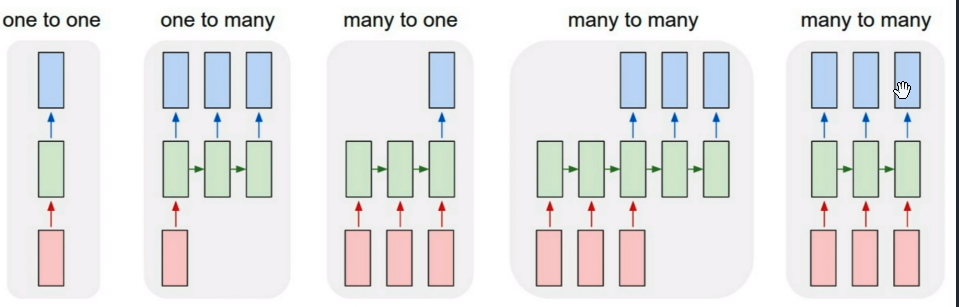
\includegraphics[width=0.7\textwidth]{images/archRNN.png}
    \caption{RNN}
\end{figure}

- **One-to-one** - classic feed forward neural network architecture, with one input and we expect one output.
- **One-to-many** - e.g. image captioning. We have one image as a fixed size input and the output can be words or sentences which are variable in length.
- **Many-to-one** e.g. sentiment classification. The input is expected to be a sequence of words or even paragraphs of words. The output can be a regression output with continuous values which represent the likelihood of having a positive sentiment.
- **Many-to-many** - machine translation like in  Google translate. The input
could an English sentence which has variable length and the output will be the same sentence in a different language which also has variable length. The last many to many model can be used for video classification on frame level. Feed every frame of a video into the neural network and expect an output right away. However, since frames are generally dependent on each other, it is necessary for the network to propagate its hidden state from the previous to the next. Thus, we need recurrent neural network for this kind of task.

Si utilizza un'architettura particolare per le RNN, chiamata \textbf{Long Short Term Memory (LSTM)}.
\begin{figure}[H]
    \centering
    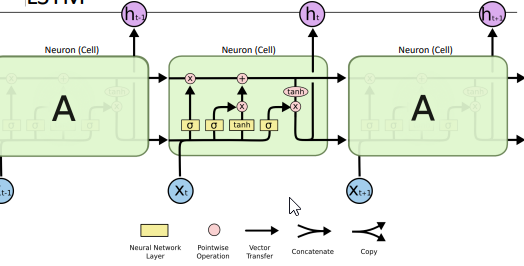
\includegraphics[width=0.7\textwidth]{images/LSTM.png}
    \caption{LSTM}
\end{figure}

 - **Forget Gate** - decides which information from long term memory be kept or discarded and this is done by multiplying the incoming long term memory (upper incoming arrow) by a forget vector generated by the current input and incoming short memory (lower arrow).

 - **Input Gate** - decides what information will be stored in long term memory. It only works with the information from the current input and short term memory from the previous step. At this gate, it filters out the information from variables that are not useful.


 - **Output Gate** - it takes the current input, the previous short term memory and newly computed long term memory to produce new short term memory which will be passed on to the cell in the next time step. The output of the current time step can also be drawn from this hidden state.


 Cose su LSTM ma boh


 \subsection{NLP}

Le reti neurali lavorano con \textbf{numeri}. Nel natural language processing si lavora con dei \textbf{testi} che sono delle \textbf{sequenze} di parole.

\textbf{Proposta 1: One Hot Encoding}:
Si potrebbe pensare ad un \textbf{one hot encoding}, ma questo sarebbe troppo 
costoso, perché se dovessimo pensare ad un OHE di un vocabolario di 1000 parole, 
questo crescerebbe in modo esponenziale

\textbf{Proposta 2:Ogni parola un unico numero}:
Problema da prendere dal notebook

\textbf{Proposta finale: Word Embedding}: Questa proposta è vincente perché permette di avere 
una rappresentazione delle parole mantenendo un'importante proprietà: la \textbf{somiglianza} tra esse. Praticamente 
un embedding è un vettore di valori in floating point. Invece di hard-codare i valori del vettore, si 
trattano come valori da \textbf{allenare}.


%tabella per "cat on mat " a 4 dimensioni 
\begin{table}[H]
    \centering
    \begin{tabular}{|c|c|c|c|}
        \hline
        cat & 0.2 & 0.1 & \\
        \hline
        on & 0.1 & 0.9 & \\
        \hline
        mat & 0.1 & 0.9 & \\
        \hline
    \end{tabular}
    \caption{Esempio di Word Embedding}
\end{table}

\subsection{Come si lavora con i Word Embedding?}

\subsubsection{Encoder}
\begin{lstlisting}[language=Python, caption={Esempio di Word Embedding}]
VOCAB_SIZE = 1000
#Per usare testo si usa un layer TextVectorization
encoder = tf.keras.layers.TextVectorization(max_tokens=VOCAB_SIZE)
encoder.adapt(train_dataset.map(lambda text, label: text))

#Parole piu usate nel dataset
vocab = np.array(encoder.get_vocabulary())
vocab[:20]

#Come sono encodate le parole
encoded_example = encoder(example)[:3].numpy()
encoded_example

#Ad esempio, l'encoding viene fatto stampando l'indice della parola nel vocabolario


\end{lstlisting}

\textbf{Nota:} Limitando il vocabolario non permette sempre di fare reverse tra indice e parola, perché la parola all'interno della frase potrebbe non essere all'interno delle top parole usate all'interno del nostro vocabolario.

\newpage

\end{document}